\documentclass[11pt,letterpaper]{article}
\usepackage{graphicx,amsmath,amsthm,amsfonts,amssymb,fullpage,xcolor,tikz,pgfplots,multirow,multicol,hyperref,caption, geometry,float,bbold}
\geometry{margin=1in}
\usepackage{setspace}
\setstretch{1.2}
\usepackage{enumerate}
\usepackage{graphicx}
\usepackage{caption}
\usepackage[operators,sets]{cryptocode}
\usepackage{authblk} % for affiliations
% \usepackage{draftwatermark}
% \usepackage[all,cmtip]{xy}

% % Customize the watermark
% \SetWatermarkText{DRAFT}          % The watermark text
% \SetWatermarkScale{5}             % Size (increase for full-page)
% \SetWatermarkColor[gray]{0.85}    % Light gray
% \SetWatermarkAngle{45}            % Diagonal placement
% \SetWatermarkFontSize{5cm}        % Optional: explicit size
% \SetWatermarkLightness{0.9}       % Optional: even lighter
% \SetWatermarkHorCenter{0.5\paperwidth} % Optional: repositioning
% \SetWatermarkVerCenter{0.5\paperheight}

% \newtheorem{thm}{Theorem}[section]
% \newtheorem{ex}{Example}[section]

\newcommand{\polys}{K[X,Y]}
\newcommand{\hpolys}{K[X\!:\!Y\!:\!Z]}
\newcommand{\productpolys}{K[X_1, Y_1, \ldots, X_n, Y_n]}


\newcommand{\dX}{\frac{\partial}{\partial X}}
\newcommand{\dY}{\frac{\partial}{\partial Y}}
\newcommand{\dXP}{\frac{\partial}{\partial X_P}}
\newcommand{\dYP}{\frac{\partial}{\partial Y_P}}
\newcommand{\dXQ}{\frac{\partial}{\partial X_Q}}
\newcommand{\dYQ}{\frac{\partial}{\partial Y_Q}}
\newcommand{\dZ}{\frac{\partial}{\partial Z}}

\newcommand{\free}[1]{{\textcolor{red}{#1}}}
\newcommand{\luke}[1]{{\textcolor{purple}{#1}}}
\newcommand{\rigo}[1]{{\textcolor{blue}{#1}}}
\newcommand{\brando}[1]{{\textcolor{green}{#1}}}




%%% Freeman's Macros %%%
\theoremstyle{definition}
\newtheorem{theorem}{Theorem}[subsection]
\newtheorem{proposition}[theorem]{Proposition}
\newtheorem{definition}[theorem]{Definition}
\newtheorem{remark}[theorem]{Remark}
\newtheorem{corollary}[theorem]{Corollary}
\newtheorem{problem}[theorem]{Problem}
\newtheorem{lemm}[theorem]{Lemma}
\newtheorem{defn}[theorem]{Definition}

\def\do#1{\csdef{#1}{\mathbb{#1}}}
\docsvlist{N,A,P,Z,Q,G,H}
\def\do#1{\csdef{#1}{\mathcal{#1}}}
\docsvlist{E,M,R,C,S,F,V,R,W,S,L,B,O}

\newcommand{\ff}{K(\E)}

\pgfplotsset{compat=1.18}
\setlength\parindent{1.5em}

\newcommand{\Fq}{\mathbb{F}_q}
\newcommand{\Fqm}{\mathbb{F}_{q^m}}
\newcommand{\Fqn}{\mathbb{F}_{q}^n}
\newcommand{\Fqmn}{\mathbb{F}_{q^m}^n}
\newcommand{\Fp}{\mathbb{F}_p}
\newcommand{\Fpn}{\mathbb{F}_{p}^n}
\newcommand{\6}{\mathbf}
\newcommand{\7}{\mathcal}
\newcommand{\rar}{\rightarrow}
\newcommand{\lar}{\leftarrow}
\newcommand{\lsamp}{\xleftarrow{\$}}
\newcommand{\map}{\mapsto}
\newcommand{\til}[1]{{\tilde{#1}}}
\newcommand{\hsh}[1]{\text{Hash}{(#1)}}
\renewcommand\epsilon\varepsilon
\newcommand{\ip}[2]{{\langle {#1}, \, {#2} \rangle}}
\newcommand{\dimFp}[1]{{\text{dim}_{\mathbb{F}_p}(#1)}}

\newcommand{\com}[1]{{\mathsf{commit}(#1)}}


\newcommand{\divi}[1]{{\text{div}(#1)}}
\newcommand{\lr}[1]{{\langle #1 \rangle}}

\captionsetup[table]{name = Algorithm}


\newcommand{\zon}{\{0, \, 1\}^n}
\newcommand{\zo}{\{0, \, 1\}}
\newcommand{\one}{\mathbb{1}}
\newcommand{\zero}{\mathbb{0}}

\newcommand{\bon}{2y_Pf(P)(3x_P^2+\alpha-2\lambda y_P)}
\newcommand{\btw}{2y_Py_Rf(R)(3x_P^2+\alpha-2y_P \lambda ) \Delta X}
\newcommand{\bth}{2y_Qf(Q)(3x_Q^2+\alpha - 2\lambda y_Q)}
\newcommand{\bfo}{2y_Qy_Rf(R)(3x_Q^2+\alpha  - 2\lambda y_Q) \Delta X}
\newcommand{\con}{2y_Pf_X(P) + (3x_P^2+\alpha) f_Y(P)}
\newcommand{\ctw}{- 2\lambda y_P(2y_Rf_X(R) + (3x_R^2+\alpha) f_Y(R))(3x_P^2+\alpha - 2y_P(\lambda + \Delta X))}
\newcommand{\cth}{2y_Qf_X(Q) + (3x_Q^2+\alpha) f_Y(Q)}
\newcommand{\cfo}{2\lambda y_Q(2y_Rf_X(R) + (3x_R^2+\alpha)f_Y(R))(3x_Q^2+\alpha - 2y_Q(\lambda + \Delta X))}

\newcommand{\non}{2 y_R \Delta X f(P)f(Q)f_X(R)(4 y_P y_Q  \Delta Y - y_P  \Gamma_Q \Delta X  - y_Q  \Gamma_P \Delta X )}
\newcommand{\ntw}{\Gamma_R \Delta X f(P)f(Q)f_Y(R)(4 y_P y_Q \Delta Y - y_P \Gamma_Q \Delta X  - y_Q \Gamma_P \Delta X )}
\newcommand{\nth}{2 y_P y_R \Delta X f(Q)f(R)f_X(P)(\Gamma_Q \Delta X - 2 y_Q \Delta Y)}
\newcommand{\nfo}{y_R \Gamma_P \Delta X f(Q)f(R)f_Y(P)(\Gamma_Q \Delta X  - 2  y_Q \Delta Y)}
\newcommand{\nfi}{2 y_Q y_R \Delta X  f(P)f(R)f_X(Q)(\Gamma_P \Delta X - 2 y_P \Delta Y) } 
\newcommand{\nsi}{y_R \Gamma_Q \Delta X f(P)f(R)f_Y(Q)(\Gamma_P  \Delta X - 2  y_P \Delta Y) }

\newcommand{\den}{y_R f(P)f(Q)f(R)(\Gamma_P\Delta X - 2 y_P \Delta Y)(\Gamma_Q\Delta X - 2 y_Q \Delta Y)}







\newcommand{\VerEquA}{2 y_T \Delta Y  \neq \Gamma_T \cdot \Delta X \text{ for any } T \in \left\{P,Q,R\right\}}
\newcommand{\VerEquB}{\Delta X \neq  (\Delta X \cdot y_i - \Delta Y \cdot x_i - \Delta X \cdot \mu) A_i \text{ for some }1 \leq i \leq n}
\newcommand{\VerEquC}{D \cdot D^{-1} \neq 1}
\newcommand{\VerEquD}{\left(\sum_{i=1}^{6} N_i\right) D^{-1} \neq \sum_i m_i A_i}






\title{
SLVer Bullet: \underline{S}traight-\underline{L}ine \underline{Ver}ification for \underline{Bullet}proofs
}
\author{Brandon Goodell, Rigo Salazar, Freeman Slaughter, Luke Szramowski
}
\affil{$\mathsf{Cypher \ Stack}$}

\date{\today}




\begin{document}

\maketitle


% \section*{Disclaimer}

% This paper is not yet completed; future updates to this document are forthcoming soon.

\section*{Change log}

This document will be updated occasionally, especially when security-sensitive results come to light. We summarize such changes here.
\begin{itemize}

\item 22 July 2025. Fixed typos and improved notation overall, added computational improvement arguments, added section on interpolation, rederived equations and improved operation count.


\item 28 June 2025. Fix broken proofs, many mistakes, tighten bounds, fill in some gaps, etc.

\item 11 June 2025. Initial preprint.
\end{itemize}


\section{Introduction}


In \cite{Eagen}, Eagen proposed a method for checking whether a sum of points in an elliptic curve group has been computed correctly. Eagen's method verifiably checks elliptic curve group operations only with linear combinations in the base field, allowing very general proofs to be encoded in inner product argument systems and rank-$1$ constraint systems (R1CS). We call this method ``straight-line verification,'' due to how it utilizes straight lines in the verification procedure.
In \cite{Kayaba}, Parker used Eagen's method in a R1CS to verify scalar multiplication of group elements, proposing a protocol based on Eagen's arguments. 
Although the iterative witness construction algorithm proposed in \cite{Eagen} is correct, the arguments are rather informal, lacking precise protocol descriptions, claims, proofs, or efficiency analyses. 
We present a method based on \cite{Eagen} for straight-lining  cryptographic protocols, offloading computational costs faced by verifiers to provers, which is useful for light-weight devices or when verification must be performed repeatedly. Computational improvements are largely due to replacing expensive division operations with lower-cost arithmetic by applying logarithmic derivatives.


Our work is not fully novel, but is a healthy expansion of previous work. In \cite{SoundnessForDLP}, Bassa contributed towards formalizing Eagen's method, explicitly describing Parker's proof of scalar multiplication and sketching arguments towards proofs of soundness.
% We expressly compute the completeness and soundness error for this approach, because, while welcome, we do not believe that Bassa's analysis was without errors.
% We then apply this approach to zero-knowledge proof systems to highlight the computational advantage offered by divisors, offloading the bulk of the computational bottleneck on the verifier's side to the prover.
% In particular, we implement the divisors framework with the Schnorr scheme and Bulletproofs, as they are most applicable to cryptocurrencies such as Monero or Salvium, though note that these are not the only protocols who may benefit from this perspective.
% We formalize a divisors-based modification to an existing proof-of-computation scheme. The original scheme, described first publicly by Eagen in \cite{Eagen}, checks whether a sum of points in some elliptic curve group $\G$ defined over a finite field $K$ has been computed correctly, using only linear combinations over $K$. The approach allows for pre-computation, so that users of a zero-knowledge proving scheme may optionally offload computational cost from verifiers to provers.
% In \cite{Kayaba}
% This approach was utilized in Parker \cite{Kayaba} for proving group point relationships within rank $1$ constraint systems. 
However, the soundness arguments in \cite{SoundnessForDLP} are not without  obstacles. In \cite{Eagen}, rational solutions to certain systems of polynomial equations are assumed to exist.
These equations do not admit rational solutions in general. Bassa lifted to the surface of pairs of elliptic curve group points to avoid this problem, but the verification equations proposed in \cite{Eagen} and studied in \cite{SoundnessForDLP} are not sufficiently justified in those documents. 


The verification equations described in \cite{SoundnessForDLP} reduce to our verification equations, and therefore are equivalent. In particular, given a variable choice of a line in the affine plane with three distinct, non-identity, and collinear points on an elliptic curve $\E$, say $P, Q, R$ with interpolating slope $\lambda$ and $x$-coordinates $X_P$, $X_Q$, and $X_R$, are necessarily dependent: $\lambda^2 = X_P + X_Q + X_R$. Thus, given any derivation $d$ on the function field $K(\E)$ over $K$, we have $dX_R = -dX_P - dX_Q$, allowing computations to reduce further than in \cite{SoundnessForDLP}.


Nonetheless, Bassa's amended approach results in formal arguments, if not proofs, of security. We fully justify the verification equations presented by Bassa, show they reduce further, and reconsider the security of Eagen's approach under the reduced verification equations. We encourage the reader to keep in mind that our verification equations are equivalent reduced versions of those presented by Bassa. Along the way, we exploit the technique in \cite{Eagen} further to reduce the total number of field divisions required by prover to one. The technique is easily applied to transform verification in 
discrete-logarithm-based protocols for generic speed-ups.

We present the protocol, and explicitly compute the completeness and soundness errors. We remark on how to complete the scheme, and our soundness error beats previous estimates in \cite{Eagen} and \cite{SoundnessForDLP}.
We also show how the corrected scheme can be used to verify scalar multiplication as in Parker's proposed protocol.
We then apply this approach to zero-knowledge proof systems like Schnorr identification and Bulletproofs to illustrate the computational advantage offered by divisors, because these protocols are simple, secure, popular, and readily applicable in cryptocurrencies such as Monero or Salvium. 
% The efficiency gains here are most applicable to currencies such as Monero or Salvium, though note that these are not the only protocols who may benefit from this perspective,


% We expand upon Bassa's work in \cite{SoundnessForDLP} by presenting a corrected version of Bassa's protocol, and explicitly computing the completeness and soundness error.
% We exemplify the approach with a simple, non-zero-knowledge proof of scalar multiplication.
% We then transform zero-knowledge proof systems, allowing provers to pre-compute data for verifiers, such that verification is a straight-line program with computations over the base field. 
% This offloads the bulk of the computational cost faced by verifiers to the prover.
% The transformation is somewhat general, but we exemplify the approach with a transformed Schnorr identification protocol and a transformed range proving system via bulletproofs. The Schnorr and bulletproofs protocols  are simple, secure, popular, and applicable (as in cryptocurrencies like Monero or Salvium), so they make for good demonstrations. We then analyze the efficiency of the approach against the un-transformed versions of these protocols.

\section{Notation and Preliminary Definitions}

We begin assuming the reader has knowledge of basic algebra concepts related to groups, rings, and fields. Our notation and background primarily follows \cite{Silverman}, but we depart notationally in a few notable ways, especially with regard to divisors. Let $\N = \left\{1, 2, 3, \dots\right\}$, let $\N_0 = \N \cup \left\{0\right\}$, and let $\mathbb{Z}_p$ be the ring of integers modulo prime $p$. 
% All sets herein are finite unless otherwise specified. 
Let $\zero$ and $\one$ represent the vectors solely composed of zeroes and ones, respectively. 

\subsection{Polynomials and Rational Functions}

For a set $S$, we use $x \lsamp S$ to mean that the element $x$ is an independent uniformly-distributed sample from set $S$. For a ring $R$, we write $R^\times = R\setminus\left\{0\right\}$ to denote the multiplicative subgroup. 
Let $p$ be a prime, $K$ a finite field with $\text{char}(K) = p$, algebraic closure $\overline{K}$, and multiplicative subgroup $K^\times = \left\{x \in K \mid x \neq 0\right\}$. Let $X, Y, Z$ be indeterminates over $\overline{K}$. Finite linear combinations in products of $X$, $Y$, and $Z$ are \textit{polynomials}. We use the following usual notation for rings of polynomials over $\overline{K}$ and $K$.
\begin{itemize}

\item  $\overline{K}[X,Y] = \left\{\sum_{i=0}^{n}\sum_{j=0}^{m} a_{i,j} X^i Y^j \mid a_{i,j} \in \overline{K}\right\}$

\item $\polys = \left\{\sum_{i=0}^{n}\sum_{j=0}^{m}a_{i,j} X^iY^j \mid a_{i,j} \in K\right\}$

\item  $\overline{K}[X,Y,Z] = \left\{\sum_{i=0}^{n}\sum_{j=0}^{m} \sum_{k=0}^{l} a_{i,j,k} X^i Y^j Z^k \mid a_{i,j,k} \in \overline{K}\right\}$

\item $K[X,Y,Z] = \left\{\sum_{i=0}^{n}\sum_{j=0}^{m} \sum_{k=0}^{l} a_{i,j,k} X^i Y^j Z^k \mid a_{i,j,k} \in K\right\}$

\end{itemize}  

For $f \in \polys$, say $f = \sum_i \sum_j a_{ij} X^iY^j$, define $\text{deg}(f) = \max \left\{i+j \mid a_{ij} \neq 0\right\}$ (and similarly for the other polynomial rings). Each of these rings (say $R$) admits a structure-preserving map $\text{deg}:R \to \N_0 = \N \cup \left\{0\right\}$ such that $\text{deg}(fg) = \text{deg}(f) + \text{deg}(g)$ and $\text{deg}(f+g) \leq \max\left\{\text{deg}(f), \text{deg}(g)\right\}$, where we follow the convention that the degree of the zero polynomial is $- \infty$. Also, $\text{deg}(f) = 0$ if and only if $f$ is a non-zero constant polynomial.


If $d \in \mathbb{N}_0$ and $f \in \overline{K}[X,Y]$, and for all $\lambda \in \overline{K}^\times$ we have that $f(\lambda X, \lambda Y) = \lambda^d f(X,Y)$, then we say $f$ is \textit{homogeneous with degree} $d$; otherwise, \textit{inhomogeneous}. Define an equivalence relation on the subset of homogeneous polynomials in $\overline{K}[X,Y,Z]$ such that every $f(X,Y,Z)$ relates to $\lambda f(X, Y, Z)$ for every $\lambda \in \overline{K}^\times$. Denote the equivalence class of $f$ under this equivalence relation with $f(X\!:\!Y\!:\!Z)$, and the set of equivalence classes under this relation with $\overline{K}[X\!:\!Y\!:\!Z]$.
Define $\text{deg}:\overline{K}[X\!:\!Y\!:\!Z] \to \N_0$ by declaring $\text{deg}(f(X\!:\!Y\!:\!Z)) = \text{deg}(f(X,Y,Z))$. Similarly define $K[X\!:\!Y\!:\!Z]$ and its degree function. 
The rings $\overline{K}[X,Y]$, $K[X,Y]$, $\overline{K}[X,Y,Z]$, and $K[X,Y,Z]$ are all integral domains. We also define the respective fields of rational functions $\overline{K}(X,Y)$, $K(X,Y)$, $\overline{K}(X,Y,Z)$, and $K(X,Y,Z)$ as usual.




\subsection{Affine and Projective Planes}

Define $\A^2(\overline{K}) = \left\{(x,y) \in \overline{K}^2\right\}$, $\A^3(\overline{K}) = \left\{(x,y,z) \in \overline{K}^3\right\}$, $\A^2(K) = \left\{(x,y) \in K^2\right\}$, and $\A^3(K)=\left\{(x,y,z) \in K^3\right\}$.  We say the elements of $\mathbb{A}^2(\overline{K})$ are \textit{affine points} and the elements of $\mathbb{A}^2(K)$ are \textit{$K$-rational} affine points. 
For any ideal $I \subseteq \overline{K}[X,Y]$, the \textit{affine vanishing set} of $I$ is  $v_a(I) = \left\{(x,y) \in \mathbb{A}^2(\overline{K}) \mid f(x,y) = 0\text{ for all } f \in I\right\}$. If $f(X,Y) \in \overline{K}[X,Y]$, we define the affine vanishing set for $f$ as the affine vanishing set for the principally generated $I = (f)$, which we denote with $v_a(f)$.


Given affine vanishing set $V$, let $I(V) = \left\{f \in \overline{K}[X,Y] \mid f(x,y) = 0\text{ for all }(x,y) \in V\right\}$  be the \textit{ideal of $V$}. It is easy to check that $I(V)$ is an ideal of $\overline{K}[X,Y]$.
We say an affine vanishing set $V$ is \textit{defined over} $K$, denoted with shorthand $V/K$, if $I(V)$ is generated as an ideal in $\overline{K}[X,Y]$ by a subset of $K[X,Y]$. 
For any affine vanishing set $V$, let $I(V/K) = I(V) \cap K[X,Y]$. It is easy to show that $I(V/K)$ is an ideal. Moreover, $V$ is defined over $K$ if and only if $I(V)$ is generated as an ideal in $\overline{K}[X,Y]$ by $I(V/K)$, i.e.\ $I(V) = I(V/K)\overline{K}[X,Y]$. 

We say $V$ is an \textit{affine variety} if $I(V)$ is a prime ideal in $\overline{K}[X,Y]$. The \textit{affine coordinate ring} of an affine variety $V/K$ is the quotient ring $K[V] = \frac{K[X,Y]}{I(V/K)}$. The \textit{function field} of $V$ is the field of fractions associated with $K[V]$, i.e.\ the set of all formal fractions $\frac{f}{g}$ where $f, g \in K[V]$ and $g \neq 0$, under an equivalence relation defined by relating $\frac{f_1}{g_1}$ to $\frac{f_2}{g_2}$ if and only if $f_1 g_2 - f_2 g_1 = 0$. We denote the function field $K(V)$.

Define an equivalence relation on $\A^3(\overline{K}) \setminus \left\{\zero\right\}$ by relating $(x,y,z)$ to $(x^\prime, y^\prime, z^\prime)$ if and only if there exists $\lambda \in \overline{K}^\times$ such that $(x^\prime, y^\prime, z^\prime) = (\lambda x, \lambda y, \lambda z)$. Denote the equivalence class of $(x,y,z)$ with $(x\!:\!y\!:\!z)$. Use $\P^2(\overline{K})$ to denote the set of equivalence classes under this relation. Similarly define $\P^2(K)$ in the evident way. We say the elements of $\P^2(\overline{K})$ are \textit{projective points} and the elements of $\P^2(K)$ are the \textit{$K$-rational} projective points. For any homogeneous ideal $I \subseteq \overline{K}[X,Y,Z]$, the \textit{projective vanishing set} of $I$ is $v_p(I) = \left\{(x\!:\!y\!:\!z) \in \P^2(\overline{K}) \mid f(x,y,z)=0\text{ for all }f \in I\right\}$. Since the generating set for $I$ contains only homogeneous polynomials, the presence of any representative in $(x\!:\!y\!:\!z)$ which kills all $f \in I$ implies all representatives kill all $f \in I$. For any $f \in \overline{K}[X,Y,Z]$, we define the projective vanishing set for $f$ as the projective vanishing set for the ideal $I=(f)$, and we use the notation $v_p(f)$.



% Given a projective vanishing set $V$, we overload notation and define $I(V)$ to be the homogeneous ideal of $\overline{K}[X\!:\!Y\!:\!Z]$ generated by the set $\left\{f \in \overline{K}[X\!:\!Y\!:\!Z] \mid f(x\!:\!y\!:\!z) = 0\text{ for all }(x\!:\!y\!:\!z) \in V\right\}$.
% We say a projective vanishing set $V$ is \textit{defined over} $K$, denoted with shorthand $V/K$, if $I(V)$ is generated as an ideal in $\overline{K}[X\!:\!Y\!:\!Z]$ by a subset of $K[X\!:\!Y\!:\!Z]$. 
% We say $V$ is a \textit{projective variety} if its homogeneous ideal $I(V)$ is a prime ideal in $\overline{K}[X,Y,Z]$. The \textit{projective coordinate ring} of an projective variety $V/K$ is the quotient ring $K[V] = \frac{K[X\!:\!Y\!:\!Z]}{I(V/K)}$. %The \textit{function field} of $V$ is the field of fractions $K(V)$, i.e.\ the set of all formal fractions $\frac{f}{g}$ where $f, g \in K[V]$ and $g \neq 0$, under an equivalence relation defined by relating $\frac{f_1}{g_1}$ to $\frac{f_2}{g_2}$ if and only if $f_1 g_2 - f_2 g_1 = 0$.


Affine points $P=(x,y) \in \A^2(\overline{K})$ (or $\A^2(K)$, respectively) naturally map to projective points $P^*=(x\!:\!y\!:\!1) \in \P^2(\overline{K})$ (or $\P^2(K)$, respectively). This map is injective, but $\P^2$ contains many copies of $\A^2$ and this map is not unique. Projective points $P=(x\!:\!y\!:\!z) \in \P^2(\overline{K})$ with $z \neq 0$ naturally map to affine points $P_*=(\frac{x}{z}, \frac{y}{z}) \in \A^2(\overline{K})$ in a similar way, but surjectively. The same statement as above holds with $\A^2(K)$ and $\P^2(K)$ replacing their counterparts everywhere.

There exists natural \textit{homogenization} maps carrying $f \in \polys$ (or $f \in \overline{K}[X,Y]$) to a homogeneous $f^* \in K[X,Y,Z]$ (or $f^* \in \overline{K}[X,Y,Z]$, respectively) where $f^* = Z^{\text{deg}(f)}f(\frac{X}{Z}, \frac{Y}{Z})$. This map is injective.
We can also dehomogenize a homogeneous polynomial $g \in \hpolys$ (or $\overline{K}[X,Y,Z]$) to a polynomial in the affine coordinate ring $g \mapsto g_*(X,Y) = g(X\!:\!Y\!:\!1) \in \polys$ (or $\overline{K}[X,Y]$, respectively). This map is surjective.
The distinguished polynomial $e(X,Y) = Y^2 - X^3 - \alpha X - \beta$ has homogenization $e^*(X,Y) = Y^2Z - X^3 - \alpha XZ^2 - \beta Z^3$. The map $(x,y) \hookrightarrow (x\!:\!y\!:\!1)$ sends zeroes of $f \in K[X,Y]$ to zeroes of $f^* \in K[X\!:\!Y\!:\!Z]$.

Using these maps, we can translate $\A^2$ to $\P^2$ and back again.  In this way, we define \textit{projective closure} of an affine variety $V$ as the projective vanishing set $\overline{V}$ such that $I(\overline{V}) = \left\{f^* \mid f \in I(V)\right\}$. We also define the function field for a projective variety $V \subseteq \P^2$ as the function field for the affine restriction \footnote{This restriction is more delicate in general than discussed here; see \cite{Silverman}.}.

% We define function fields for product varieties $V^n$ in the natural way as in \cite{Silverman}, namely 

\subsection{Plane Curves}
\label{sec:planecurve}

A \textit{plane affine curve} $\F$ is just the affine vanishing set of some $f \in \overline{K}[X,Y]$, i.e.\ $\F = v_a(f)$.  If $g$ is a multiplicative factor of $f$, then the curve $\mathcal{G}$ corresponding to $g$ is called a \textit{component} of $\mathcal{F}$.

We define the \textit{intersection number} of a curve $\F$, simple/non-singular points of $\F$, singular points of $\F$, and the multiplicity of a point $P$ on $\F$ as in \cite{hirschfeld2008algebraic}. In particular, if $\ell \in \overline{K}[X,Y]$ is a line which is not a component of $\mathcal{F}$, the \textit{multiplicity} of $P$ is $\min{m \mid \ell\text{ a line through }P}$ where $m$ is the intersection number of $\ell$ and $\F$ at $P$. Multiplicity theory is a rich rabbit hole  preceding Zariski, so we do not go into further detail. 
% Moreover, given $P = (x,y) \in \overline{K}^2$, there exists a map $\text{ord}_P:\overline{K}(X,Y) \to \Z$ called the \textit{order of vanishing} at $P$ defined as follows.
% \begin{align}
% \text{ord}_P(f) =& \begin{cases} m > 0; & P\text{ is a root of }f\text{ with multiplicity }m \\ m < 0; & P\text{ is a pole of }f\text{ with multiplicity }\left|m\right|=-m \\ 0; & \text{otherwise} \end{cases}
% \end{align} We define $\text{ord}_P(f)$ for subrings of $\overline{K}(X,Y)$ by restricting $\text{ord}_P$.

In the sequel, we use the distinguished family of polynomials parameterized by $\alpha, \beta \in K^2$ of the form $e = Y^2 - X^3 - \alpha X - \beta \in K[X,Y]$ such that $4\alpha^3 + 27\beta^2 \neq 0$; these are exactly the non-singular elliptic curves. We note that some authors consider the term ``elliptic curve" to refer specifically to non-singular elliptic curves, while others do not; see \cite{Silverman,DummitNotes}. While we make a distinction for pedagogical reasons, we do not consider singular elliptic curves here.

Plane affine curves may have any of the properties of affine vanishing sets discussed above. 
A \textit{plane projective curve} $\F$ is just the projective vanishing set of some homogeneous $f \in \overline{K}[X\!:\!Y\!:\!Z]$, i.e.\ $\F = v_p(f)$. In both cases, we define $\text{deg}(\F) = \text{deg}(f)$. Plane projective curves may have any of the properties of projective vanishing sets discussed above. 

Recall the distinguished family of polynomials $e = Y^2 - X^3 - \alpha X - \beta \in K[X,Y]$ such that $4\alpha^3 + 27\beta^2 \neq 0$. Define $\E=v_p(e)$ as the plane projective curve of the homogenization $e^*$. It is easy to show that the only $(x\!:\!y\!:\!z) \in \E$ with $z=0$ is $(0\!:\!1\!:\!0)$.  We call this the \textit{point at infinity} on $\E$, and we denote $O = (0\!:\!1\!:\!0)$. It is also easy to show that $\E$ is a projective variety, $I(\E/K) = (e) \subseteq K[X\!:\!Y\!:\!Z]$ is the associated ideal over $K$, and the associated function field is as follows.
\begin{align}
K(\E) =& \left\{\frac{f(X,Y) + (e)}{g(X,Y) + (e)} \mid f, g \in K[X,Y], g \notin (e) \right\}
\end{align}

Except in the case of confusion or for clarification, we often omit the ideal $(e)$ from our notation in the sequel, writing $f/g \in K(\E)$, with the understanding that the numerator and denominator of every element in the function field is a coset modulo this ideal.

However, representing a function field element with coefficient representations of two arbitrary bivariate polynomials is expensive. Indeed if $m = \text{deg}(f)$ and $f$ is bivariate, then we can write $f = \sum_{i=0}^{m} \sum_{j=0}^{i} c_{i,j}X^{i-j}Y^j$, requiring $1 + 2 + 3 + \cdots + m + (m+1) = \frac{1}{2}(m+1)(m+2)$ coefficients from $K$. Thus, if $\text{deg}(f), \text{deg}(g) \leq m$, then we can represent $\frac{f}{g}$ with $(m+1)(m+2)$ coefficients from $K$. On the other hand, more efficient representations are available. Indeed, if $f \in K[X,Y]$, then as $K[X,Y] = K[X][Y]$, we have the following.
\begin{align*}
f(X,Y)
=& \sum_{j=0}^{m} b_{j}(X)Y^j\text{ where }b_j \in K[X]\text{ for }0 \leq j \leq m  \\
=& \sum_{j=0}^{\lceil m/2\rceil} b_{2j}(X)Y^{2j} + b_{2j+1}(X)Y^{2j+1} \text{ where }b_{m+1}=0\\
=& \sum_{j=0}^{\lceil m/2\rceil} Y^{2j}\left(b_{2j}(X) + b_{2j+1}(X)Y\right)\\
=& \sum_{j=0}^{\lceil m/2\rceil} \left(X^3 + \alpha X + \beta\right)^j\left(b_{2j}(X) + b_{2j+1}(X)Y\right) \\
=& \underbrace{\left(\sum_{j=0}^{\lceil m/2\rceil} \left(X^3 + \alpha X + \beta\right)^jb_{2j}(X)\right)}{} + \underbrace{\left(\sum_{j=0}^{\lceil m/2\rceil} \left(X^3 + \alpha X + \beta\right)^jb_{2j+1}(X)\right){}Y} \\
=& \quad \quad \quad \quad \quad \quad a(X)  \quad \quad \quad \quad \quad \quad + \quad \quad \quad \quad \quad \quad b(X)Y
\end{align*} where $a(X) = \sum_{j=0}^{\lceil m/2\rceil} (X^3 + \alpha X + \beta)^j b_{2j}(X) \in K[X]$ and $b(X) = \sum_{j=0}^{\lceil m/2\rceil} (X^3 + \alpha X + \beta)^j b_{2j+1}(X) \in K[X]$. Representing a polynomial $f$ this way requires $\text{deg}(a) + \text{deg}(b)+2$ elements of $K$. So, we can forget our above representation of elements of the function field $\frac{f}{g}$ with $f, g \in K[X,Y]$, and use $\frac{a_1(X) + b_1(X)Y}{a_2(X) + b_2(X)Y}$ for some $a_1, a_2, b_1, b_2 \in K\left[X\right]$, representing the function field element with only $\text{deg}(a_1)+\text{deg}(a_2)+\text{deg}(b_1)+\text{deg}(b_2)+4$ elements of $K$ instead. 

We may go further, however. For each $a(X) + b(X)Y + (e)$, we have an element $a(X) - b(X)Y + (e) \in \polys/(e)$ satisfying the following due to the ideal $I(\E/K) = (e)$ and the multiplicative absorption property of ideals.
\begin{align*}
(a_1(X) + b_1(X)Y + (e))(a_1(X) - b_1(X)Y + (e)) =& a_1^2 - b_1^2Y^2 + (e) \\
=& a_1^2 - (X^3 + \alpha X + \beta)b_1^2 + (e)
\end{align*}
Hence, for any $\frac{a_1(X)+b_1(X)Y + (e)}{a_2(X)+b_2(X)Y + (e)} \in K(\E)$, we can apply an identity map by multiplying and dividing by $(a_2(X) - b_2(X)Y + (e))$, yielding another representative whose denominator does not depend on $Y$ as follows
\begin{align*}
& \frac{a_1(X)+b_1(X)Y + (e)}{a_2(X)+b_2(X)Y + (e)} \cdot \frac{a_2(X)-b_2(X)Y + (e)}{a_2(X)-b_2(X)Y + (e)} \\ &= \frac{a_1(X)a_2(X) - a_1(X) b_2(X) Y + a_2(X)b_1(X) Y - b_1(X) b_2(X) Y^2 + (e)}{(a_2(X))^2 - (b_2(X))^2Y^2 + (e)} \\
% =& \frac{a_0a_1 - (X^3 + \alpha X + \beta)b_0b_1 - (a_0b_1 - a_1b_0)Y+(e)}{a_1^2 - (X^3 + \alpha X + \beta)b_2^2+(e)}\\
&= \frac{f_1(X) + f_2(X)Y + (e)}{f_3(X) + (e)}
\end{align*} where $f_1(X) = a_1(X) a_2(X) - (X^3 + \alpha X + \beta)b_1(X)b_2(X)$, $f_2(X) = a_2(X)b_1(X) - a_1(X) b_2(X)$, and $f_3(X) = (a_2(X))^2 - (X^3 + \alpha X + \beta)(b_2(X))^2$. This requires only $\text{deg}(f_1(X))+\text{deg}(f_2(X))+\text{deg}(f_3(X))+3$ elements of $K$.

Thus, we write every element of $K(\E)$ as $\frac{f_1(X) + f_2(X)Y + (e)}{f_3(X) + (e)}$ for some polynomials $f_0(X)$, $f_1(X)$, $f_2(X) \in K[X]$.
Later, we outperform this slightly, as we practically only consider elements such that $\text{deg}(f_3(X) + (e)) = 0$, i.e.\ $f_3(X) + (e) = 1 + (e)$, requiring only $\text{deg}(f_1)+\text{deg}(f_2)+2$ coefficients to describe $f$.


% \subsection{Derivations}
% Given any field extension $K \subseteq L$, an additive group homomorphism $d: L \to L$ is said to be a \textit{derivation over} $K$ if $d(K) = \left\{0\right\}$ and $d$ satisfies Leibniz' rule: $d(ab) = d(a)b + ad(b)$. Given an intermediate field, $K \subseteq F \subseteq L$, such that $d(F) \subseteq F$, the restriction of $d$ over $K$ on $L$ to $F$ yields a derivation over $K$ on $F$.  In the case $L=\overline{K}(X,Y)$, derivations $\dX$ and $\dY$ are defined as usual (and $\dZ$ is defined over $\overline{K}(X,Y,Z)$ similarly).
% All derivations are linear combinations of these derivations $\dX$, $\dY$, and $\dZ$. Indeed, 
% \begin{itemize}
%     \item[(i)] for any $a, b \in L$, every linear combination $a(X,Y) \dX + b(X,Y) \dY$ is a derivation over $K$ on $L$, and 
%     \item[(ii)] every derivation over $K$ on $L$ is of the form $a(X,Y) \dX + b(X,Y) \dY$, for some $a, b \in \overline{K}(X,Y)$. 
% \end{itemize}
% For $F \subseteq \overline{K}(X,Y)$, the  derivations satisfying $dF \subseteq F$ are precisely the derivations with corresponding $(a, b) \in F^2$.

% Similarly, $\overline{K}(X,Y,Z)$ has derivations of the form $d=a\dX + b\dY + c\dZ$ for some $a, b, c \in \overline{K}(X,Y,Z)$, and if all $a, b, c$ are in an intermediate field $K \subseteq F \subseteq \overline{K}(X,Y,Z)$, then $d$ is a derivation on $F$.

% Given any derivation $d:L \to L$ over $K$, there is a natural map $\delta:L \to L$ mapping $f \mapsto \frac{df}{f}$. Note that given any $f, g \in L$, we have that 
% $$ \delta(fg) = \frac{d(fg)}{fg} = \frac{gdf + fdg}{fg} = \frac{df}{f} + \frac{dg}{g} = \delta(f) + \delta(g).$$
% In particular, $\delta$ is a group homomorphism from the multiplicative subgroup of $L$ to the additive group of $L$.


% \subsection{Planes, plane Curves, coordinate rings, and function fields}

% The \textit{affine plane} over $K$ consists of \textit{affine points} and \textit{affine lines}, where the points are exactly the elements of $K^2$ and the lines are polynomials with degree $1$; that is, $\left\{f \in \polys \mid \text{deg}(f) = 1\right\}$. 
% If $f(X,Y) \in \polys$, the \textit{affine vanishing set} is $v_a(f) = \left\{(x,y) \in K^2 \mid f(x,y) = 0\right\}$. We say an affine point $(x,y)$ \textit{lies on} a line $\ell$ if $(x,y) \in v_a(\ell)$.
% We say $\polys$ is the \textit{affine coordinate ring}.  

% The \textit{projective plane} over $K$ consists of \textit{projective points} and \textit{projective lines}. The projective points are equivalence classes from $K^3/\sim$, where $(x,y,z) \sim (x^\prime, y^\prime, z^\prime)$ if and only if there exists $\lambda \in K\setminus \{0\}$ such that $(x^\prime, y^\prime, z^\prime) = (\lambda x, \lambda y, \lambda z)$.
% The projective lines are homogeneous polynomials with degree $1$, so that is, $\left\{f \in \hpolys \mid \text{deg}(f)=1\right\}$. If $f(X:Y:Z) \in \hpolys$, the \textit{projective vanishing set} is $v_p(f) = \left\{(x:y:z) \in K^3 \mid f(x:y:z)=0\right\}$. We say a projective point $(x:y:z)$ \textit{lies on} a line $\ell$ if $(x:y:z) \in v_p(\ell)$. We say $\hpolys$ is the \textit{projective coordinate ring}.


% Affine points $(x,y)$ naturally map to a projective point $(x\!:\!y\!:\!1)$ and map $f \in \polys$ to a homogeneous polynomial in the projective coordinate ring $f \mapsto f^*(X:Y:Z) = Z^{\text{deg}(f)}f(\frac{X}{Z}, \frac{Y}{Z})$. We say these maps are \textit{homogenization} maps. We can also dehomogenize a projective point $(x:y:z)$ with $z \neq 0$ to an affine point $(\frac{x}{z}, \frac{y}{z})$ and dehomogenize a homogeneous polynomial $g \in \hpolys$ to a polynomial in the affine coordinate ring $g \mapsto g_*(X,Y) = g(x\!:\!y\!:\!1)$.

% A \textit{plane affine curve} $\F$ is the affine vanishing set of some $f \in \polys$, and we write $\F = v_a(f)$. If $f$ is irreducible,  $\F$ has \textit{affine coordinate ring} $K[\F] = \polys/(f)$.
% If $f$ is irreducible, then $K[\F]$ is an integral domain with field of fractions $K(\F) = \text{Frac}(K[\F])$; we call $K(\F)$ the \textit{function field} of $\F$ (or of $f$) over $K$. We let $\overline{K}(\F)$ denote the algebraic closure of $K(\F)$.
% Certainly, there is a field monomorphism $K(\F) \hookrightarrow \overline{K}(X,Y)$, 
% so derivations $d$ over $K$ on $\overline{K}(X,Y)$ yields a derivation over $K$ on $K(\F)$. In particular, every derivation $d$ over $K$ on $K(\F)$ is of the form $a \dX + b\dY$ for some $(a, b) \in K(\F)$.
% If $f_1, f_2, f_3$ are polynomials (all affine or all projective) such that $f_1 \mid f_2$ and $f_1 \mid f_3$, then we say that the curve $\F_1$ is a \textit{common component} of $\F_2$ and $\F_3$.

% A \textit{plane projective curve} is the projective vanishing set of some $f \in \hpolys$, and we write $\F = v_p(f)$. As in the affine case, $\F$ has a \textit{projective coordinate ring}, for which we overload notation by writing $K[\F] = \hpolys/(f)$. If $f \in \hpolys$ is irreducible, then $K[\F]$ is an integral domain with field of fractions $K(\F) = \text{Frac}(K[\F])$, which we call the function field of $\F$ over $K$. 
% We define common components by divisibility as in the affine case.


% Recall from Section \ref{sec:planecurve} we defined $e = Y^2 - X^3 - \alpha X - \beta \in K[X,Y]$.  Let $\E = v_a(e)$. Note that function field elements $f \in K(\E) = \text{Frac}(\polys/(e))$ are of the form $f = \frac{f_0(X,Y) + (e)}{f_1(X,Y) + (e)}$ for some $f_0, f_1 \in \polys$. For $t\in\{0,1\}$, say $f_t(X,Y) = \sum_{i=0}^{n_t}\sum_{j=0}^{m_t} f_{t,i,j}X^iY^j$ for some $f_{t,i,j} \in K$, we define $f_{tj}(X) = \sum_{i=0}^{n_t}f_{t,i,j}X^i$. We have:
% \begin{align}
% f_t(X,Y) =& \sum_{ij} f_{t,i,j}X^iY^j = \sum_{j} f_{t,j}(X)Y^j\\
% =& \sum_{j} f_{t,2j}(X)Y^{2j} + f_{t,2j+1}(X)Y^{2j+1} \\
% =& \sum_{j} Y^{2j}\left(f_{t,2j}(X) + f_{t,2j+1}(X)Y\right)\\
% =& \sum_j \left(X^3 + \alpha X + \beta\right)^j\left(f_{t,2j}(X) + f_{t,2j+1}(X)Y\right) \\
% =& \left(\sum_j \left(X^3 + \alpha X + \beta\right)^jf_{t,2j}(X)\right) + Y\left(\sum_j \left(X^3 + \alpha X + \beta\right)^jf_{t,2j+1}(X)\right)
% \end{align}
% So, we can forget our previous representation $f_0, f_1$ and write $f \in \ff$ as $f = \frac{f_0 + Yf_1 + (e)}{f_2 + Yf_3 + (e)}$ for some other $f_0, f_1, f_2, f_3 \in K\left[X\right]$ instead. In fact, even better is true. For each, we have an element $f_2 - Yf_3 + (e) \in \polys/(e)$ satisfying the following:
% \begin{align}
% (f_2 + Yf_3 + (e))(f_2 - Yf_3 + (e)) =& f_2^2 - Y^2f_3^2 + (e) \\
% =& f_2^2 - (X^3 + \alpha X + \beta)f_3^2 + (e) 
% \end{align}

% Thus, we can reduce $f$ by applying an identity map, multiplying and dividing by this conjugate, to clear $Y$ from the denominator.

% \begin{align}
% f \cdot \frac{f_2 - Yf_3 + (e)}{f_2 - Yf_3 + (e)} =& \frac{f_0 + Yf_1 + (e)}{f_2 + Yf_3 + (e)} \cdot\frac{f_2 - Yf_3 + (e)}{f_2 - Yf_3 + (e)} \\
% =& \frac{f_0f_2 - (X^3 + \alpha X + \beta)f_1f_3 + Y(f_0f_3 + f_1f_2) + (e)}{f_2^2 - (X^3 + \alpha X + \beta)f_3^2 + (e)}
% \end{align}
% By this rationalization of the denominator procedure, without loss of generality, we can forget even the above representation, and write every $f$ as $f = \frac{f_0 + Yf_1 + (e)}{f_2 + (e)}$ for some other  polynomials $f_0, f_1, f_2 \in K[X]$ instead.

% Of course, storing $f(X,Y)$ and $g(X,Y)$ requires $O(\text{deg}(f)^2 + \text{deg}(g)^2)$ coefficients, but describing each $f_i$ requires only $\text{deg}(f_i)$ coefficients. This representation reduces the storage requirements to describe $f$ dramatically. We therefore represent $f \in \ff$ with $f_0, f_1, f_2 \in K[X]$.

\subsection{Elliptic Curve Groups}

For the remainder of this manuscript, we assume all elliptic curve groups have prime order strictly greater than $3$.


Recall the distinguished polynomial $e(X,Y) = Y^2 - X^3 - \alpha X - \beta \in \polys$ where $4\alpha^3 + 27\beta^2 \neq 0$, and consider the plane projective curve $\E = v_p(e)$. Note $I(\E/K) = (e)$. This $\E$ is an elliptic curve with affine coordinate ring $K[\E] = \frac{K[X,Y]}{(e)}$ and function field $K(\E) = \text{Frac}(K[\E])$. 
For a natural number $n \in \mathbb{N}$, the surface $\mathcal{E}^n$ is a variety with coordinate ring $K\left[\E^n\right] = \productpolys/I(\E^n/K)$, where $I(\E^n/K)$ is the ideal generated by the set $\left\{e(X_i, Y_i) \mid i \in [n]\right\}$, and function field $K(\E^n) = \text{Frac}(\productpolys/I(\E^n/K))$.

We additionally take B\'{e}zout's theorem for granted (see Theorem I.7.8 in \cite{Hartshorne}).
\begin{theorem}[{B}{\'{e}}zout's {T}heorem]
Let $\F_1$, $\F_2$ be distinct curves in $\P^2(\overline{K})$, having 
degrees $n_1, n_2$, respectively. Let $\F_1 \cap \F_2 = \left\{P_1, \dots, P_s\right\}$, and say, for each $1 \leq i \leq s$, that point $P_i$ has multiplicity $m_i$. Then $\sum_{i=1}^{s} m_i = n_1n_2$. 
\end{theorem}

The projective variety corresponding to $\E$ is $\G(\E) = v_p(e)$. Then $e^*$ is the homogenization of $e$ defined earlier. This $\G(\E)$ admits an abelian group operation $+$ following the elliptic curve group law, which determines decompositions of the group identity in $\G(\E)$ as follows. First, the point at infinity $O=(0\!:\!1\!:\!0)$ is distinguished as the group identity. Next, collinear points define decompositions of $O$. Bezout's theorem implies every line intersects $v_p(\E)$ at $3$ points, counting multiplicities. Hence, every set of collinear points is a triple $(P, Q, R) \in \G^3$ such that $P + Q + R = O$. We have three cases: $P$ has multiplicity $3$, $2$, or $1$.
\begin{itemize}
\item If $P = Q = R$, then $3P = O$, i.e.\ $P$ has multiplicity $3$. This is contraindicated for a non-singular elliptic curve $\E$ of prime order $p > 3$.

\item If $P = Q$, then $P + P + R = 2P + R = O$, so $2P = -R$. In this case, we sum points with themselves, however this implies that the line $\ell$ interpolating $P$ and $R$ intersects $\E$ at $P$ with multiplicity $2$. Since $\E$ is non-singular, it must be that $\ell$ is \textit{tangent} to $\E$ at $P$.

\item If $P$, $Q$, and $R$ are all distinct, we have two sub-cases: one of these points is an inverse of another, or not.
\begin{itemize}
\item If $P = -Q$, then $P + Q + R = O$ implies that $R = O$. In this case, the line interpolating $P$, $Q$, and $R$ includes the point at infinity $O$. The lines passing through $O$ and intersecting $\E$ at a non-identity point are precisely the \textit{vertical lines}. Similarly for the case $P = -R$. 
\item All other cases are when $P$, $Q$, and $R$ are distinct, not inverses of each other, and correspond to lines which are neither vertical nor tangent. 
\end{itemize}
\end{itemize}
% For any non-identity point $P \in \G(\E) \setminus \{O\}$, it must be that $P$ lies on some unique projective line $\ell$ which is tangent to $\E$. Bezout's theorem implies $\ell$ intersects $\E$ at $P$ with multiplicity $2$ and at a second point $R$ with multiplicity $1$. In this case, the elliptic curve group law states $P + P + R = O$, so $R = -2P$. Then, given points $P, Q \in \G(\E)$, there exists a unique projective line $\ell$ that interpolates $P$ and $Q$. The line may or may not be vertical, where vertical lines satisfy a trivial relation. If this line is vertical, then the elliptic curve group law declares $P + Q = O$, so $Q = -P$. Otherwise, B\'{e}zout's's theorem ensures that $\ell$ intersects $\E$ at a third point $R$ (which may or may not be distinct from $P$ and $Q$). In this case, the elliptic curve group law declares $P + Q + R = O$, so $R = -(P+Q)$. 
That is to say, to find $-P$, we use the other root on the line passing through $P$ which is \textit{vertical}; to sum a point $P$ with itself we use the other root on the line passing through $P$ which is \textit{tangent to} $\E$; to add two generic non-identity points $P, Q$ we use the third root $R$ of the line $\ell$ interpolating $P, Q$, setting $P + Q = -R$.
These rules are sufficient for generating the elliptic curve group $\G(\E)$. In the sequel, we denote this $\G$, as we use the same $\E$ throughout.

We emphasize that group points like $P$, $Q$, $R$ are elements of $v_p(e)$, and thus are points from the projective plane, of the form $(x\!:\!y\!:\!z)$. All points $(x,y)$ from $\A^2$ are embedded as $(x\!:\!y\!:\!1)$, and the only solution to $e^*$ in $\P^2$ with $z= 0$ is exactly $(0\!:\!1\!:\!0)$, so if $P$, $Q$, and $R$ are non-identity, then these have $z \neq 0$. That is to say, each $(x\!:\!y\!:\!z)$ has a representative $(\frac{x}{z}, \frac{y}{z}, 1)$, and we may re-label our variables to assume the non-identity points can all be written $(x\!:\!y\!:\!1) \in \P^2$. Such a point admits the dehomogenization, an affine point $(x,y) \in \A^2$ (which can, in turn, be re-embedded into $\P^2$). 
For this reason, we often conflate non-identity points like $P$, $Q$, $R \in v_p(e)$ with their dehomogenizations $(x_P, y_P)$, $(x_Q, y_Q)$, and $(x_R, y_R)$, clarifying whether we are handling affine or projective points with context in the text.


\begin{figure}[htbp]
\centering
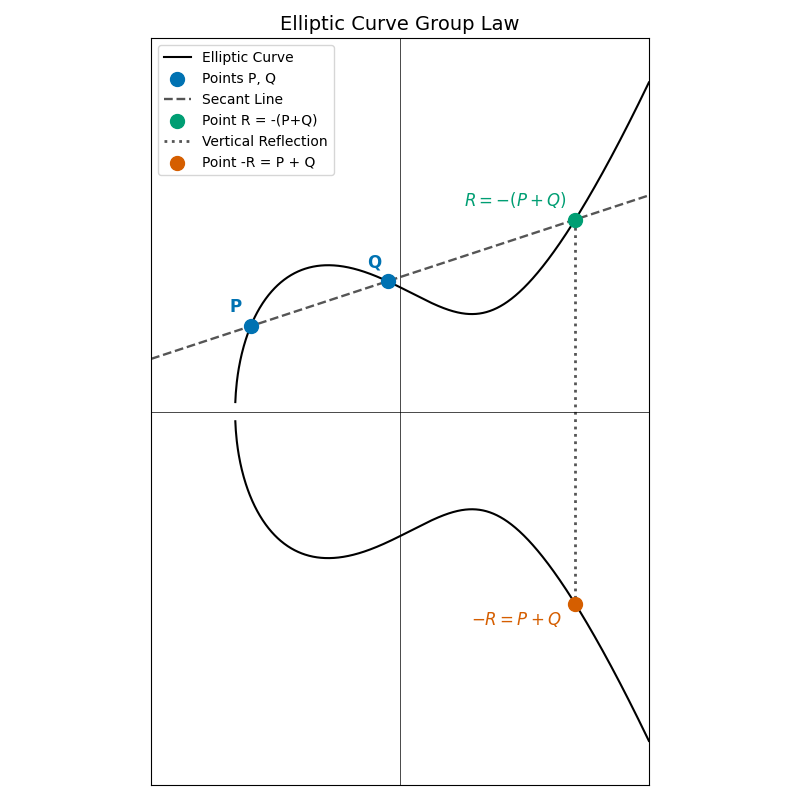
\includegraphics[width=\textwidth]{ecg.png}
\caption{The points $P, Q, R$ are collinear, so their sum is $P + Q + R = O$, where $O$ is the group identity. In particular, $R = -(P+Q)$ and its reflection across the $X$-axis is $-R = P+Q$. \label{fig:grouplaw}}
\end{figure}



% If $\F_1 = \E$ and $\F_2$ is a line $\ell$, then $\sum_i m_i = 3$. The partitions of $3$ in $\N$ are $1 + 1 + 1$, $1 + 2$, and $3$, so every line intersects $\E$ at $3$ points, counting multiplicities. To fully work out the group structure requires identities, inverses, and the group operation as defined for arbitrary pairs.


% First, the point at infinity in projective space $O=(0\!:\!1\!:\!0) \in \P^2(K)$ is distinguished as the group identity\footnote{See \cite{Silverman} and \cite{Hartshorne} for details, general constructions, and more.}. Next, we find the additive inverse of a non-identity $P \in \G$, i.e.\ we seek $Q \in \G$ such that $P + Q + O = O$. Then  $P = -Q$. By B\'{e}zout's theorem, we need a line interpolating $P, Q, O$, and the multiplicities of these points sum to $3$. So we have three cases.

% If $P$ has multiplicity $3$, then $P = Q = O$, a contradiction. If $P$ has multiplicity $2$, then $P = Q$ yet $P + Q + O = P + P = 2P = O$.  If $4\alpha^3 + 27\beta^2 \neq 0$, then $\E$ is not singular, a contradiction. So $P$, $Q$, and $O$ form a $3$-set of intersection points, and each has multiplicity $1$. It is easy to check that a  line in $\P^2(\overline{K})$ intersects $\E$ at $O$ if and only if the line is vertical. Thus, to invert $P$, we just reflect $P=(x_P,y_P) \in \P^2$ across the $X$-axis, setting $-P = (x_P, -y_P)$.

% This establishes the group identity and inverse elements. It remains to establish the group operation on arbitrary pairs of points, $P$, $Q$. We can assume $P \neq -Q$ as we handled that case already. Given these, to compute $R$ such that $P + Q + R = O$, we find a line $\ell$ interpolating $P$ and $Q$ and consider B\'{e}zout's theorem: the line and $\E$ may intersect at $P$ with multiplicity $3$, $2$, or $1$.

% In the first case, $\ell$ intersects $\E$ at $P$ with multiplicity $3$. In this case, $P + P + P = O$ implies $3P = O$, so $P$ is $3$-torsion, implying $\E$ is singular. If $4\alpha^3 + 27\beta^2 \neq 0$, then $\E$ is not singular, a contradiction. 

% In the second case, $\ell$ intersects $\E$ at $P$ with multiplicity $2$. In this case $P + P + Q = O$, and so the line interpolating $P$ and $Q$ is tangent to $\E$ at $P$, with multiplicity $2$. That is to say, the second case occurs when we add a point $P$ to itself, ``doubling'' it, computing $P + P = 2P = -Q$. 

% In the final case, the line $\ell$ intersects $\E$ at three distinct points $P$, $Q$, and $R$, necessarily with multiplicity $1$ each by B\'{e}zout's theorem. That is to say, the line $\ell$ intersects $\E$ transversally at $P$, $Q$, $R$. For these points, $P + Q + R = O$, so $R = -(P+Q)$. Moreover, we can write the coordinates $R=(x_R, y_R)$ with $y_R = \lambda x_R + \mu$ where $(\lambda, \mu) \in \overline{K}^2$ parameterize the line interpolating $P$ and $Q$.

% These rules are sufficient for generating the elliptic curve group $\G(\E)$. 

However, the $y$ coordinates are \textit{almost} uniquely determined by their corresponding $x$ coordinate. Indeed, for each $T \in \left\{P, Q, R\right\}$, only two elements of $K$ satisfy $y_T^2 = x_T^3 + \alpha x_T + \beta$. Distinguishing which $y_T$ corresponds to the point $T$ simply requires a convention for interpreting a parity/sign bit.
Thus, representing $(x_T,y_T)$ requires only one more bit than representing $x_T$ alone.

In the sequel, we leave $\E$ implicit and denote this $\G$, as we use the same $\E$ throughout. Moreover, the group law as described here is equivalent to a group law defined for rational functions, not merely lines; the proof of this is beyond the scope of this text. See \cite{Silverman} for details.

\subsubsection{Group Law and Summing Points}\label{subsec:detail}

We use lines to compute $P + Q$ explicitly as a rational function for a pair $(P, Q) \in (\G \setminus \left\{O\right\})^2$ such that $P \neq \pm Q$; this is useful in our derivations in Appendix \ref{sec:derivation} later. As both are not the identity and $P \neq \pm Q$, the line interpolating $P$ and $Q$ is not vertical. By B\'{e}zout's theorem, the line must intersect $\E$ at an additional point $R$, which may coincide with $P$ or $Q$. In the case where the three points are distinct, then these intersection points all have a multiplicity of $1$. The group law states $P + Q + R = O$. 
We compute $(x_R, y_R)$ to represent $R$.


Note that, as elements of $\G$, we may write \[P = (x_P\!:\!y_P\!:\!z_P) = \left\{(x,y,z) \mid \forall \lambda \in K^\times, (x,y,z) = (\lambda x_P,\lambda y_P,\lambda z_P)\right\}\] and $Q = (x_Q\!:\!y_Q\!:\!z_Q)$ similarly. As non-identity elements, $P \neq O = (0\!:\!1\!:\!0)$ so $z_P \neq 0$, and the equivalence class $(x_P\!:\!y_P\!:\!z_P)$ contains a representation of the form $(x,y,1)$ (and similarly for $Q$. Thus, we lose no generality by assuming $z_P=z_Q=1$, in which case we can write $P = (x_P\!:\!y_P\!:\!1)$ and $Q=(x_Q\!:\!y_Q\!:\!1)$. Then $P$ and $Q$ may be dehomogenized to affine points $(x_P, y_P)$, $(x_Q, y_Q) \in \E$; we identify $P = (x_P\!:\!y_P\!:\!1)$ with $(x_P, y_P)$, and similarly for $Q$, in our discussion below, keeping in mind that we are actually transferring between points on the projective plane to points on the affine plane via the dehomogenization and homogenization maps.

Define $\lambda = \frac{y_P - y_Q}{x_P - x_Q}$ and $\mu = y_P - \lambda x_P$ as functions of $P$ and $Q$.
These $\lambda, \mu$ parameterize the interpolating line $\ell(X,Y) = Y - \lambda X - \mu \in K[X,Y]$, and therefore $y_T = \lambda x_T + \mu$ for each $T \in \left\{P, Q, R\right\}$.  Also, since $e(x_T, y_T) = 0$, we have $(\lambda x_T + \mu)^2 = x_T^3 + \alpha x_T + \beta$. Thus, the points $P, Q, R$ have $x$ coordinates which are distinct roots of the third degree polynomial $X^3 - \lambda^2 X^2 + (\alpha - 2\lambda \mu)X + (\beta - \mu^2)$ in $X$.
All the roots are accounted for, so the polynomial splits into linear factors. 
\begin{align*}
(X-x_P)(X-x_Q)(X-x_R) &= X^3 - \lambda^2 X^2 + (\alpha - 2\lambda \mu)X + (\beta - \mu^2) 
% X^3 - (x_P + x_Q + x_R)X^2 + (x_Px_Q + x_Px_R + x_Qx_R)X - x_Px_Qx_R
\end{align*}
The linear independence of $\left\{1,X,X^2,X^3\right\}$ implies we may match coefficients, so $-\lambda^2 = -x_P - x_Q - x_R$, where $x_P$ and $x_Q$ are already given. 
\begin{align*}
\begin{cases}
x_R &= \lambda^2 - x_P - x_Q \\ 
y_R &= \lambda x_R + \mu
\end{cases}
\end{align*}
Recalling $\lambda$ and $\mu$ defined above are rational functions, it is clear that these are both rational in $(x_P, s_P, x_Q, s_Q)$, as promised. 
% Moreover, if $P, Q, R$ are distinct, non-identity, and collinear, say on line $Y - \lambda X - \mu$, then the coordinates all satisfy the following:
% \begin{align*}
% X^3 - (\lambda X + \mu)^2 + \alpha X + \beta =& (X-x_P)(X-x_Q)(X-x_R)\\
% X^3 - \lambda^2 + ... =& X^3 - (x_P + x_Q + x_R)X^2 + ...
% \end{align*} where the ellipses denote lower degree terms. 
Moreover, the group law and the elliptic curve equation demand the following constraints are satisfied.
\begin{align}
\begin{cases} 
\lambda =& \frac{y_Q-y_P}{x_Q-x_P} \\
\mu =& y_P - \lambda x_P \\
y_P =& \lambda x_P + \mu\\
y_Q =& \lambda x_Q + \mu\\
y_P^2 =& x_P^3 + \alpha x_P + \beta \\
y_Q^2 =& x_Q^3 + \alpha x_Q + \beta
\label{thesystem}
\end{cases}
\end{align}
% Note that if $x_P, y_P, x_Q, y_Q$ are variables, then these are al rational functions.

We emphasize that, in our notation, lowercase terms like $(x_T, y_T)$ denote the coordinate pairs of a point denoted with an uppercase term $T$, whereas uppercase terms like $(X_T, Y_T)$ refer to variable pairs of transcendental elements, which we handle as coordinate pairs of unspecified points.


\subsection{Divisors over Elliptic Curves}

For each $T = (x\!:\!y\!:\!z) \in \G$, let $\left[T\right]$ be a formal symbol corresponding to $T$. A \textit{divisor} is a finite sum of these formal symbols. These sums can be summed, so divisors generate an additive group which we call $\text{Div}_K(\E)$. We use functions $\nu: \G \to \Z$ with finite supports to represent a divisor $[\nu] = \sum_{T \in \G} \nu(T) \left[T\right]$. The \textit{degree} of $\left[\nu\right]$ is $\text{deg}(\left[\nu\right])=\sum_{T \in \G} \nu(T)$. 
Let $\text{Div}_{K}^0(\E)$ denote the set of degree-zero divisors. Note $\text{Div}_{K}^0(\E) \subseteq \text{Div}_K(\E)$ and is closed under addition, i.e.\ is a subgroup.

Given any $f \in K(\E)^\times$, we can define a map $\E \to \Z$  by mapping $T \mapsto \text{ord}_T(f)$, and this has with finite support as the numerator and denominator of $f$ both have finite degree (and hence a $f$ has a finite number of roots and poles, even counting multiplicity). Denote $\text{div}(f) = \sum_{T \in \E} \text{ord}_T(f)[T]$.  Define $\text{Prin}(\E) = \left\{\text{div}(f) \mid f \in K(\E)\right\}$. Note we have the following chain of subgroups: $\text{Prin}(\E) \subseteq \text{Div}_K^0(\E) \subseteq \text{Div}_K(\E)$. In the sequel, define the following relation.
\begin{align*}
\R_{\text{div}} =& \left\{(f, [\nu]) \mid f \in K(\E)^\times, \ [\nu] \in \text{Div}_K^0(\E), \text{ and } \text{div}(f) = [\nu]\right\} 
\end{align*}
Later, we are particularly interested in the following sub-relation.
\begin{align}
\R^\prime =& \left\{(f, [\nu]) \mid f \in K(\E)^\times, \ [\nu] \in \text{Div}_K^0(\E), \ \left|\text{supp}(\nu)\right| \geq 3, \text{div}(f) = [\nu],  f \neq g^p\quad\forall g \in K(\E)^\times\right\} \label{theRelation}
\end{align}

% Later we find it convenient to restrict this relation to pairs $(f, [\nu])$ such that $f$ is not a $p^{th}$ power. 
We take the following for granted.
\begin{theorem}
Let $f \in K(\E)$ be nonzero, $v_a(f) \setminus \left\{O\right\} = \left\{P_1, \ldots, P_n\right\}$, and $v_a(f^{-1}) \setminus \left\{O\right\} = \left\{Q_1, \ldots, Q_s\right\}$ with $n + s \geq 1$. If each $P_i$ has multiplicity $m_i  \in \N$ and each $Q_j$ has multiplicity $t_j \in \N$, and $\sum_i m_i - \sum_j t_j \neq 0$, then:
\begin{enumerate}[(a)]
\item $\sum_i m_i - \sum_j t_j > 0$ implies $f$ has a pole at $O$ with multiplicity $\sum_i m_i - \sum_j t_j$, 
\item $\sum_i m_i - \sum_j t_j < 0$ implies $f$ has a root at $O$ with multiplicity $\sum_j t_j - \sum_i m_i$, and
\item $\sum_i m_i P_i - \sum_j t_j Q_j = O$.
\end{enumerate}
In particular, $\text{div}(f) = \sum_i m_i [P_i] - \sum_j t_j [Q_j] - (\sum_i m_i - \sum_j t_j)[O]$, $\text{deg}(\text{div}(f)) = 0$, and $\text{div}(f)$ represents a nontrivial decomposition of $O \in \G$, namely $\sum_i m_i P_i - \sum_i t_j Q_j = O$.
\end{theorem}

% Principal divisors admit an abelian group structure and form a subgroup $\texttt{Prin}_K(\E) \subseteq \text{Div}_K^0(\E)$. 

If $f_1, f_2 \in \ff$ have $(v_p(f_1^*) \cup v_p(1/f_1^*)) \cap (v_p(f_2^*) \cup v_p(1/f_2^*)) = \emptyset$, we say $f_1$ and $f_2$ have \textit{disjoint roots and poles}. If $f_1$ and $f_2$ have disjoint roots and poles, it is easy to check that $v_p(f_1^*f_2^*) = v_p(f_1^*)\cup v_p(f_2^*)$ and $v_p(1/(f_1^* f_2^*)) = v_p(1/f_1^*)\cup v_p(1/f_2^*)$. Thus, for such an $f_1, f_2$ pair, we have that $\text{div}(f_1f_2) = \text{div}(f_1)+\text{div}(f_2)$. More generally, $\text{div}$ is a group homomorphism from the multiplicative subgroup of the function field $K(\E)^\times$ to the additive (sub)group $\text{Prin}(\E)$.

Note that if $f_1$ and $f_2$ do not have disjoint roots and poles, then the common roots and poles may partially or completely cancel in the product $f_1f_2$. This expresses itself as terms canceling in the sum $\text{div}(f_1) + \text{div}(f_2)$.



\subsection{Weil Reciprocity}

Every $f \in K(\E)$ induces a homomorphism. Indeed, let $[\eta] = \sum_{T \in \G} \eta(T)[T]$ be any divisor such that the support of $\eta$ is disjoint from the roots and poles of $f$. Then let $\widehat{f}([\eta]) = \prod_{T\in \G} f^*(T)^{\eta(T)}$; this is well-defined because the points of $[\eta]$ are disjoint from the roots and poles of $f$.

\begin{theorem}
For each $f \in K(\E)$, if $[\eta_1]$ and $[\eta_2]$ have supports that are disjoint from the roots and poles of $f$, then $\widehat{f}([\eta_1+\eta_2]) = \prod_{T \in \G} f^*(T)^{\eta_1(T)+\eta_2(T)} = \widehat{f}([\eta_1])\widehat{f}([\eta_2])$.
\label{thm:inducedmaphom}
\end{theorem}


For the remainder of this document, we assume that $[\eta_1]$ and $[\eta_2]$ have mutually disjoint supports.


\begin{theorem}[Weil Reciprocity Law]
Let $f, g \in K(\E)^\times$ with disjoint supports that also exclude $O$, where $\text{div}(f) = \sum\limits_T \nu(T) [T]$ and $\text{div}(g) = \sum_T \eta(T) [T]$. Then \[\widehat{f}(\text{div}(g)) = \prod\limits_{T \in \G} f^*(T)^{\eta(T)} = \prod\limits_{S \in \G} g^*(S)^{\nu(S)} = \widehat{g}(\text{div}(f)).\] 
\end{theorem}

In particular, if $g$ has a degree $1$ polynomial representing its numerator $aX + bY + c + (e)$ and $1 + (e)$ as the denominator, then $\widehat{g}([\nu]) = \prod_T (ax_T + by_T + c)^{\nu(T)}$.
For the remainder of this document, when we refer to $f, g \in K(\E)^\times$, we will assume that they have disjoint supports which  exclude $O$, the point at infinity.



\subsection{Derivations}

Polynomials admit formal derivatives and partial derivatives as usual: if $f = \sum_i a_i X^i$, define $f^\prime = \sum_i i a_i X^{i-1}$, and if $f = \sum_{i,j} a_{i,j}X^i Y^j$, define $\dX f = \sum_{i,j} ia_{i,j}X^{i-1} Y^j$ and $\dY f = \sum_{i,j} ja_{i,j}X^iY^{j-1}$.

More generally, given any field extension $K \subseteq L$, an additive group homomorphism $d: L \to L$ is said to be a \textit{derivation over} $K$ if $d(K) = \left\{0\right\}$ and $d$ satisfies Leibniz' rule: $d(ab) = d(a)b + ad(b)$. Given an intermediate field, $K \subseteq F \subseteq L$, such that $d(F) \subseteq F$, the restriction of $d$ over $K$ on $L$ to $F$ yields a derivation over $K$ on $F$.  In the case $L=\overline{K}(X,Y)$, derivations $\dX$ and $\dY$ are defined as usual (and $\dZ$ is defined over $\overline{K}(X,Y,Z)$ similarly).
All derivations are linear combinations of these derivations $\dX$, $\dY$, and $\dZ$. Indeed, 
\begin{itemize}
    \item[(i)] for any $a, b \in L$, every linear combination $a(X,Y) \dX + b(X,Y) \dY$ is a derivation over $K$ on $L$, and 
    \item[(ii)] every derivation over $K$ on $L$ is of the form $a(X,Y) \dX + b(X,Y) \dY$, for some $a, b \in \overline{K}(X,Y)$. 
\end{itemize}
For $F \subseteq \overline{K}(X,Y)$, the  derivations satisfying $d(F) \subseteq F$ are precisely the derivations with corresponding $(a, b) \in F^2$.

Similarly, $\overline{K}(X,Y,Z)$ has derivations of the form $d=a\dX + b\dY + c\dZ$ for some $a, b, c \in \overline{K}(X,Y,Z)$, and if all $a, b, c$ are in an intermediate field $K \subseteq F \subseteq \overline{K}(X,Y,Z)$, then $d$ is a derivation on $F$. 

Later, derivations are used with elements of the function field $K(E)$, where the variables $X$ and $Y$ are not independent (they satisfy a polynomial relation, namely the defining equation of the curve. \cite{bassapersonal}), but those derivations are inherited from the usual ones on $\overline{K}(X,Y)$.

Given any derivation $d:L^\times \to L$ over $K$, there is a natural map $\delta:L^\times \to L$ mapping $f \mapsto \frac{df}{f}$. Note that given any $f, g \in L$, we have that 
$$ \delta(fg) = \frac{d(fg)}{fg} = \frac{d(f)g + fd(g)}{fg} = \frac{d(f)}{f} + \frac{d(g)}{g} = \delta(f) + \delta(g).$$
In particular, $\delta$ is a group homomorphism from the multiplicative subgroup of $L$ to the additive group of $L$.


\subsection{Schwartz-Zippel}

We take the following for granted.

\begin{lemm}
Let $0 \neq f \in \overline{K}[Z_1, Z_2, \ldots, Z_n]$ with $\text{deg}(f) = d$, and let $S$ be a finite subset of $\overline{K}$. If $s_1, s_2, \ldots, s_n$ are sampled independently and uniformly from $S$, then the probability that $f(s_1, \ldots, s_n)=0$ is at most $\frac{d}{\left|S\right|}$.
\end{lemm}

It is not strictly necessary for $S$ to be a subset of an algebraically closed field, but this definition of Schwartz-Zippel is sensible for our purposes.



\section{Method}

Suppose that a prover and verifier wish to implement a proving scheme in an elliptic curve group setting. In most cases, verification requires satisfying one or more linear constraints coming from the group law of $\G$. That is to say, a proof includes some non-identity group elements $P_1, \ldots, P_n \in \G \setminus \left\{O\right\}$ and integer weights $m_1, \ldots, m_n \in \Z$, then the verification procedure requires checking that $\sum_{i=1}^{n} m_i P_i = O$.

The prover and verifier recall that every principal divisor $\sum_{i=1}^{n} m_i [P_i] - (\sum_{i=1}^{n} m_i)[O]$ corresponds to a decomposition of $O$, so they can merely check whether some divisor  is principal.
The map \textit{div} is a surjective group homomorphism. Therefore, there exists an element $f \in K(\E)^\times$ such that $\text{div}(f) = \sum_i m_i [P_i] - \left(\sum_i m_i\right)[O]$, which can be used as a witness of principality.

% In particular, every $P_i$ with $m_i > 0$ is a root of $f$ with multiplicity $m_i$, and every $P_i$ with $m_i < 0$ is a pole of $f$ with multiplicity $-m_i = \left|m_i\right|$. 

The prover and verifier also recall Weil reciprocity provides $\widehat{f}(\text{div}(g)) = \widehat{g}(\text{div}(f))$ for every pair $f, g \in K(\E)^\times$ without $O$ in their supports. For a fixed $f$, Weil reciprocity implies an equality of rational functions in the coefficients of $g$ and the coordinates of the points of $\text{div}(g)$; clearing denominators, we obtain a polynomial expression. Evaluating this polynomial at a given $(g, \text{div}(g))$ always yields equality. 

Thus, if $f \in K(\E)$ and some random $(g, \text{div}(g))$ is a root of the polynomial obtained by rationalizing $\widehat{f}(\text{div}(g)) - \widehat{g}(\text{div}(f))$, then the Schwartz-Zippel Lemma implies that the polynomial is the zero polynomial exactly, except with a probability inversely proportional to the cardinality of the set from which we sample $g$. 
We show that checking whether $\widehat{f}(\text{div}(g)) = \widehat{g}([\nu])$ for a random linear $g$ is sufficient to determine if $\text{div}(f) = [\nu]$, except perhaps with a probability given by the Schwartz-Zippel Lemma. Thus, the prover and verifier can conclude that $\sum_{T \in \G} \nu(T) T = O$.

Since the coefficients of $g$ are computed as rational functions in Appendix \ref{BigLambda} and Equation \ref{bigM}, hence the application of Schwartz-Zippel is ostensibly justifiable. 
A potential issue was brought to us in private communication \cite{bassapersonal} regarding sampling the coefficients of $g$ randomly before computing its roots (as opposed to sampling the roots randomly outright). 
% In the case of lines, these two cases are evidently equivalent, because of the one-to-one relationship between coefficients and roots of $ax+b$. 
% For the more general case, one can argue that Vieta's formula shows that a dependency between the coefficients implies a dependency between the roots, and vice versa.
For the general case, we present Sage code \footnote{\url{https://gist.github.com/FreemanSlaughter/b03c69878c39eb00b8ed273f983f9732}} (see  \cite{freemanslaughter_gist}) giving statistical evidence of that the two cases result in the same distribution of roots, enabling our application of Schwartz-Zippel.



\subsection{Previous Approaches}
The system of $9$ equations with $6$ unknowns in Equation \ref{thesystem} influences many computations with derivations in the sequel, in turn impacting the application of the chain rule. %Indeed, students of the standard calculus sequence may be familiar with using the \textit{Jacobian} of similar systems of equations to determine if a system is smooth at a point. This yields chain-rule equations when differentiating function field elements at $P$, $Q$, and $R$. 
In particular, if $\lambda$ and $\mu$ are handled as independent variables, four more variables must be determined in order to solve the system (among $x_P, x_Q, x_R, y_P, y_Q, y_R$). This forces at least once choice of $x_T$ for $T \in \left\{P,Q,R\right\}$ to be handled as a dependent variable, totally determined by the other variables. However, this $x_T$ is (in general) irrational in $\lambda$ and $\mu$.

The work in \cite{Eagen} intended to characterize proofs of security handling $\lambda$ and $\mu$ as the free variables to determine solutions to this system. %This would simplify verification by allowing the chain rule to be computed with respect to the line $Y - \lambda X - \mu = 0$.
Solutions for $x_R$ in terms of $\lambda$ and $\mu$ are obtainable using Cardano's formula, but the solutions are not guaranteed to be rational functions in $\lambda$ and $\mu$ (and therefore neither. In fact, generally these solutions are not rational, which complicates the application of derivatives beyond the computations in \cite{Eagen}.

On the other hand, by picking the $x$-coordinates of $P$ and $Q$, $x_P$ and $x_Q$, and sign bits $s_P$ and $s_Q$, we can solve for the $y$-coordinates $y_P$ and $y_Q$. With $P=(x_P,y_P)$ and $Q=(x_Q,y_Q)$ in hand, we solve this system for solutions which are rational in $(P,Q)$. 



% This system of equations is important in applying derivations to function field elements, and is not to be overlooked.
% There may be other methods available with different algebraic costs which work over the general case, these constraints are only problematic with negligible probability when $P$ and $Q$ are independently sampled uniformly at random from $\G$. 



\subsection{Method Description}

Let $K$ be a finite field with characteristic $p$, and let $\E$ be a non-singular elliptic curve over $K$ such that $\left|\mathbb{G}(\E)\right| = q > 3$ for some prime $q$. Let $H:\left\{0,1\right\}^* \to K^2 \times \zo \times \zo$ be a cryptographic hash function. Define the tuple of algorithms $\Pi = (\texttt{Setup}, \texttt{Prove}, \texttt{Verify})$ as follows. 
\begin{itemize}
\item $\texttt{Setup}(\lambda) \to \texttt{params}$. Input security parameter and output setup parameters $\texttt{params}$.
\item $\texttt{Prove}(\texttt{params}, [\nu]) \to \pi$. The prover does the following:
\begin{enumerate}
\item \label{prove1} Compute \[\texttt{out} \leftarrow \texttt{Wit}(\texttt{params}, \underbrace{P_0, \ldots, P_0}_{\nu(P_0)\text{ times}}, \underbrace{P_1, \ldots, P_1}_{\nu(P_1)\text{ times}}, \cdots, \underbrace{P_{n-1}, \ldots, P_{n-1}}_{\nu(P_{n-1})\text{ times}})\] with Algorithm \ref{alg:makewitness}; if $\texttt{out} = \bot$, output $\bot$ and terminate.
\item \label{prove2} Compute $(x_P, x_Q, s_P, s_Q) \leftarrow H(\texttt{params}, f, [\nu])$. Compute the values $\pm y_P$, $\pm y_Q$ as solutions to the elliptic curve equation $y_T^2 = x_T^3 + \alpha X_T + \beta$ for $T=P,Q$, and use $s_P$ and $s_Q$ as sign bits to determine $y_P$ and $y_Q$. Set $P = (x_P, y_P)$ and $Q=(x_Q, y_Q)$. If $P = \pm Q$, output $\bot$ and terminate. \label{firststep}
\item \label{prove3} Compute $R = -(P + Q)$. If $P = \pm R$ or $Q = \pm R$ or $\left\{P, Q, R\right\} \cap \left\{P_i\right\}_{i=1}^{n} \neq \emptyset$, then output $\bot$ and terminate. %any of the follwoing conditions are satisfied, output $\bot$ and terminate. 

\item \label{prove4} Parse the following, if possible; otherwise, output $\bot$ and terminate.
\begin{align*}
% \item $f \leftarrow \texttt{out}$,
(f_1(X), f_2(X)) = f &\leftarrow \texttt{out} \\%\text{ for some }f=\frac{f_1(X)+f_2(X)Y}{f_3(X)} \\
\sum_{i=1}^{n} m_i [P_i] &\leftarrow [\nu] \\
(x_i, y_i) &\leftarrow P_i\text{ for each }1 \leq i \leq n \\
(x_P, y_P) &\leftarrow P \\
(x_Q, y_Q) &\leftarrow Q \\
(x_R, y_R) &\leftarrow R
\end{align*}
\item \label{prove5} Compute/set the following: 
\begin{align*}
\Delta X =& x_Q - x_P\\
\Delta Y =& y_Q - y_P\\
\mu =& y_P - \lambda x_P \\
f_X =& f_1^\prime(X) + Yf_2^\prime(X)\\
f_Y =& f_2(X)
\end{align*}

\item \label{prove6} Compute $\Gamma_T := 3x_T^2 + \alpha$ for each $T \in \left\{P, Q, R\right\}$. If $\Gamma_T \cdot
\Delta X  = 2 y_T \Delta Y$  or $f(T) = 0$ for any $T \in \left\{P, Q, R\right\}$, output $\bot$ and terminate.


\item \label{prove7} Compute the following:
\begin{align*}
A_i =& \Delta X \cdot(y_i \Delta X - x_i \Delta Y + y_P \Delta X - x_P \Delta Y)^{-1}\text{ for each }1 \leq i \leq n  \\
% N_1 =& \non \\
% N_2 =& \ntw \\
% N_3 =& \nth \\
% N_4 =& \nfo \\
% N_5 =& \nfi \\
% N_6 =& \nsi \\
D =& \den
\end{align*}


\item \label{prove8} Compute $D^{-1}$ and output $\pi = (f,  A_1, \ldots, A_n, D^{-1})$. 
\end{enumerate}


\item $\texttt{Verify}(\texttt{params}, [\nu], \pi) \to b \in \zo$.
\begin{enumerate}
\item \label{verify1} Parse $(f, A_1, \ldots, A_n, D^{-1}) \leftarrow \pi$ if possible; otherwise, output $0$ and terminate.
\item \label{verify2}  Execute steps \ref{firststep}-\ref{prove6} from \texttt{Prove}. If any of these computations fail, output $0$ and terminate.
% \item Compute challenge points $(P, Q) \leftarrow H(\texttt{params}, f, [\nu])$. If $P = \pm Q$, output $0$ and terminate.
% \item Compute $R = -(P + Q)$. If $P = \pm R$ or $Q = \pm R$ or $\left\{P, Q, R\right\} \cap \left\{P_i\right\}_{i=1}^{n} \neq \emptyset$, output $0$ and terminate. %any of the follwoing conditions are satisfied, output $\bot$ and terminate.
% \item Parse the following, if possible; otherwise, output $\bot$ and terminate.
% \begin{itemize}
% \item $(f,  A_1, \ldots, A_n, B_1, B_2, B_3, B_4) \leftarrow \pi$,
% \item $\frac{f_1(X) + Yf_2(X) + (e)}{f_3(X) + (e)} \leftarrow f$,
% \item $\sum_{i=1}^n m_i P_i \leftarrow [\nu]$,
% \item $(x_i, y_i) \leftarrow P_i$,
% \item $(x_P, y_P) \leftarrow P$,
% \item $(x_Q, y_Q) \leftarrow Q$, and
% \item $(x_R, y_R) \leftarrow R$.
% \end{itemize}
% \item Carry out step \ref{prove5} from \texttt{Prove}.
\item  \label{verify3} Compute $D$ as in step \ref{prove7} from \texttt{Prove} and compute the following:
\begin{align*}
N_1 =& \non \\
N_2 =& \ntw \\
N_3 =& \nth \\
N_4 =& \nfo \\
N_5 =& \nfi \\
N_6 =& \nsi 
\end{align*}
If any of these computations fail, output $0$ and terminate.

\item  \label{verify4} If any of the following hold, output $0$ and terminate.
\begin{itemize}
% \item $\lambda \Delta X \neq \Delta Y$,
\item $\VerEquA$,
\item $\VerEquB$, 
\item $\VerEquC$,
% \item $b_iB_i \neq c_i$ for some $1 \leq i \leq 4$, or
\item $\VerEquD$. 
% \free{$\sum\limits_{j=1}^4 b_j c_{j+1} c_{j+2} c_{j+3} \neq \prod\limits_{j=1}^4 c_{j} \cdot \sum\limits_i m_i A_i$, where in the $j$ sum we take indices modulo $4$ as a cyclic sum}
\end{itemize}
\item  \label{verify5} Otherwise, output $1$ and terminate.

\end{enumerate}

\end{itemize}



\begin{table}[H]
    \centering
    \begin{tabular}{|l|}
    \hline
    $\texttt{line}(P, Q) \to \texttt{out} \in \{\bot\} \cup K(\E)$ \\
    \hline
    \textbf{If} $P \notin \E$ or $Q \notin \E$, return $\bot$. \\
    \textbf{Elif} $P = Q = O$ return $1 \in K$. \\
    \textbf{Elif} $P = O$ and $Q \neq O$, return $\texttt{line}(Q, Q)$. \\
    \textbf{Elif} $P \neq O$ and $Q = O$, return $\texttt{line}(P, P)$. \\
    \textbf{Elif} $P = Q$: \\
    \quad Set $\lambda = \frac{2y_P}{3x_P^2 + \alpha}$ \\
    \textbf{Elif} $P = -Q$: \\
    \quad Set $\lambda = 0$ \\
    \textbf{Else}: \\
    \quad Compute: \\
    \quad\quad $\Delta y = y_Q - y_P$\\
    \quad\quad $\Delta x = x_Q - x_P$\\
    \quad\quad $\lambda = \frac{\Delta y}{\Delta x}$\\
    \textbf{Return} $(P, \lambda)$. \\\hline
    \end{tabular}    
    \caption{
        Input points $P=(x_P,y_P)$, $Q=(x_Q,y_Q)$, and outputs the point-slope representation of a degree $1$ polynomial. If $P = Q$, the line passes through $P$ and is tangent to $\E$; if $P = -Q$, the line is vertical and passes through both $P$ and $Q$; otherwise, the line interpolates $P$ and $Q$. 
    }
    \label{alg:makeline}
\end{table}

\begin{table}[H]
    \centering
    \begin{tabular}{|l|}
    \hline
    $\texttt{Wit}(P_0, P_1, P_2, \ldots, P_{n-1}) \to \texttt{out} \in \{\bot\} \cup K(\E)$ \\
    \hline
    \textbf{If} $n = 0$ \textbf{then return} $\bot$. \\
    \textbf{If} $(P_0 + P_1 + \dots + P_{n-1}) \neq O$ \textbf{then return} $\bot$. \\
    \textbf{If} $P_j = O$ for any $j$ \textbf{then return} $\bot$. \\
    Initialize $\texttt{queue}=\emptyset$.\\

    % Set $\texttt{modulus} := e(X,Y) = Y^2 - X^3 - \alpha X - \beta$.\\

    \textbf{Let} $j = 0$.\\
    \textbf{While} $j < n$: \\
        \quad \textbf{If} $j+1 < n$: \\
        \quad\quad Set pair $(A_{j/2},B_{j/2}) = (P_{j}, P_{j+1})$.\\
        \quad\quad Set degree $m_j = 2$. \\
        \quad \textbf{Else}:\\
        \quad\quad Set pair $(A_{j/2},B_{j/2}) = (P_{j}, O)$.\\
        \quad\quad Set degree $m_j = 1$.\\
        \quad Compute:\\
        \quad\quad $T_{j/2} = A_{j/2} + B_{j/2} \in \E$,\\
        \quad\quad $\texttt{out}\leftarrow \texttt{line}(A_{j/2},B_{j/2})$.\\
        \quad\quad If $\texttt{out} = \bot$, output $\bot$ and terminate.\\
        \quad\quad Else: \\
        \quad\quad\quad Parse $(U_j, \lambda_j) \leftarrow \texttt{out}$. \\
        \quad\quad\quad $(w_j, z_j) \leftarrow U_j$. \\
        \quad \quad\quad Form $\ell_j = (Y-z_j) - \lambda_j(X-w_j)$. \\
        \quad Enqueue $\texttt{queue} \leftarrow (m_j, T_j, \ell_j)$.\\
        \quad Increment $j$ by $2$.\\
    \textbf{While} $\texttt{len}(\texttt{queue}) > 1$:\\
        \quad Initialize $\texttt{nextQueue} = \emptyset$.\\
        \quad \textbf{If} $\texttt{len(queue)}$ is odd:\\
        \quad\quad Dequeue $x \leftarrow \texttt{queue}$.\\
        \quad\quad Enqueue $\texttt{nextQueue} \leftarrow x$.\\

        \quad \textbf{While} $\texttt{len(queue)} \geq 2$:\\
        \quad\quad Dequeue $(m_a, T_a, f_a)$, $(m_b, T_b, f_b) \leftarrow \texttt{queue}$.\\
        \quad\quad Compute:\\
        \quad\quad\quad $T_{a,b} = T_a + T_b$,\\
        \quad\quad\quad $\ell_{a,b} = \texttt{line}(T_a,T_b)$,\\
        \quad\quad\quad $\texttt{numerator} = f_a \cdot f_b \cdot \ell_{a,b}\mod e(X,Y)$,\\
        \quad\quad\quad $\texttt{denominator} = \texttt{line}(T_a,-T_a)\cdot\texttt{line}(T_b,-T_b)$,\\
        % \quad\quad Perform polynomial division:\\
        % \quad\quad\quad $(g, r) = \texttt{numerator} \;\texttt{div\_rem}\; \texttt{denominator}$.\\
        % \quad\quad\quad (Assert remainder $r = 0$)\\[1ex]

        \quad \quad\quad $m_{a,b} = m_a + m_b$.\\
        \quad\quad\quad $g = \frac{\texttt{numerator}}{\texttt{denominator}}$. \\
        % \quad\quad $\texttt{Trim}(g, 1+m_{a,b})$.\\[1ex]

        \quad\quad Enqueue $\texttt{nextQueue} \leftarrow (m_{a,b}, T_{a,b}, g)$.\\

        \quad Set $\texttt{queue} = \texttt{nextQueue}$.\\
    Pop final element $(m, T, f)$ from $\texttt{queue}$.\\
    \textbf{If} $T \neq O$ or $m \neq n$, output $\bot$ and terminate.\\
    Output $f$. \\

    \hline
    \end{tabular}    
    \caption{
        Constructing a rational function whose divisor interpolates a set of elliptic curve points. Based on \cite{Kayaba}.
    }
    \label{alg:makewitness}
\end{table}

% \begin{table}[H]
%     \centering
%     \begin{tabular}{|l|}
%     \hline
%     $\texttt{Wit}(P_0, P_1, P_2, \ldots, P_{n-1}) \to \texttt{out} \in \{\bot\} \cup K(\E)$ \\
%     \hline
%     If no points were provided, output $\bot$ and terminate. \\
%     If the input points do not sum to the identity $O$, or any input point is $O$, \\
%     \quad output $\bot$ and terminate. \\
%     Initialize an empty queue $\texttt{queue} = \emptyset$. \\
%     If $n$ is odd, set $\texttt{reserved} = P_{n-1}$ and proceed with pairs $(P_{2j}, P_{2j+1})_{j=0}^{\lfloor n/2\rfloor}$. \\
%     For each pair $(P_{2j},P_{2j+1})$ for $0 \leq j \leq \lfloor n/2 \rfloor$: \\
%     \quad Compute: \\
%     \quad\quad $T_j = P_{2j} + P_{2j+1} \in \E$,\\
%     \quad\quad $\ell_j = \texttt{line}(P_{2j},P_{2j+1}) \in K(\E)$ \\
%     \quad Enqueue $(2, T_j, \ell_j)$ to the back of $\texttt{queue}$. \\
%     % Set $e(X,Y) \leftarrow  Y^2 - X^3 - aX - b$, the curve modulus. \\
%     While $\texttt{len}(\texttt{queue}) > 1$: \\
%     % \quad Initialize empty queue $\texttt{nextQueue} = \emptyset$. \\
%     % \quad If $\texttt{len}(\texttt{queue}) \equiv 1 \mod 2$: \\
%     % \quad\quad Pop the last element from $\texttt{queue}$ and push it onto $\texttt{nextQueue}$. \\
%     % \quad Let $N = \lfloor\texttt{len}(\texttt{queue})/2\rfloor$. \\
%     % \quad For $1 \leq j \leq N$: \\
%     \quad If $\texttt{len}(\texttt{queue})$ is odd,, reserve $P_{n-1}$ 
%     \quad If $n$ is odd, reserve $P_{n-1}$. \\
%     \quad Dequeue $(m_a, T_a, f_a)$ and $(m_b, T_b, f_b)$ from the front of $\texttt{queue}$. \\
%     \quad Parse $(x_a, y_a) \leftarrow T_a$, $(x_b, y_b) \leftarrow T_b$. \\
%     \quad Compute: \\
%     \quad\quad $T_{a,b} = T_{a} + T_{b}$,\\
%     \quad\quad $\widehat{\ell}_{a,b} = \texttt{line}(T_{a}, T_{b})$,\\
%     \quad\quad $\texttt{numerator} = f_{a} \cdot f_{b} \cdot \widehat{\ell}_{a,b} \mod e(X,Y)$,\\
%     \quad\quad $\texttt{denominator} = (X-x_a)(X-x_b)$,\\
%     \quad\quad $g := \texttt{numerator}/\texttt{denominator}$.\\
%     % \quad\quad Truncate zero-coefficient terms from $q$ based on total merged points.\\
%     \quad Enqueue $(m_a+m_b, T_{a,b}, g)$ to the back of  $\texttt{queue}$. \\
%     Pop $(m, T, f) \leftarrow \texttt{queue}$. \\
%     % Truncate zero-coefficient terms from $f$ based on total number of input points. \\
%     If $T \neq O$, output $\bot$ and terminate. \\
%     Output $f$. \\
%     \hline
%     \end{tabular}    
%     \caption{Constructing a rational function whose divisor interpolates a list of elliptic curve points. Note that this algorithm is not an exact recreation of the algorithm in \cite{Kayaba}. We assume that $\texttt{line}$ inputs points $P = (x_P, y_P)$, $Q=(x_Q, y_Q)$ and outputs the interpolating line $(y_Q-y_P)(X-x_P) + (x_Q-x_P)(Y-y_P)$.}
%     \label{alg:makewitness}
% \end{table}


% \begin{table}[H]
%     \centering
%     \begin{tabular}{|l|}
%     \hline
%     $\texttt{Wit}(\texttt{params}, [\nu]) \to \texttt{out} \in \left\{\bot\right\} \cup K(\E)$ \\
%     \hline
%     Parse $\sum_{i=1}^{n} m_i P_i \leftarrow [\nu]$. \\
%     Compute $\texttt{out} \leftarrow \texttt{MakePairs}(\texttt{params}, [\nu])$. \\
%     If $\texttt{out} = \bot$, output $\bot$ and terminate. \\
%     Otherwise, parse $\left\{\texttt{pair}_j\right\}_{j=1}^M \leftarrow \texttt{out}$. \\
%     Initialize empty $\texttt{queue} = \emptyset$. \\
%     For each $1 \leq j \leq M$: \\
%     \quad Parse $(Q_{j,1},Q_{j,2}) \leftarrow \texttt{pair}_j$. \\
%     \quad Parse $(x_{j,1}, y_{j,1}) \leftarrow Q_{j,1}$ and $(x_{j,2}, y_{j,2}) \leftarrow Q_{j,2}$. \\
%      \quad Compute: 
%      \quad \quad $\ell_j = (X-x_{j,1})(y_{j,2}-y_{j,1})+(x_{j,2}-x_{j,1})(Y-y_{j,1})$ \\
%      \quad \quad $T_j = Q_{j,1} + Q_{j,2} \in \G$ \\
%     % \quad Set $\texttt{group\_law}_j = (Q_{j,1},Q_{j,2},T_j)$. \\
%     \quad  Queue $(T_j, \ell_j)$ into $\texttt{queue}$. \\
%     % \quad Set $\texttt{result} = 1 \in K$. \\
%      While $\texttt{len}(\texttt{queue}) > 1$: \\
%     \quad If $\texttt{len}(\texttt{queue}) \equiv 1 \ (\text{mod }2)$, set $\texttt{reserved} \leftarrow \texttt{queue}[-1]$ \\
%     \quad Let $N = \texttt{len}(\texttt{queue})/2$. \\
%     \quad For $1 \leq j \leq N$: \\
%     \quad \quad Pop $(T_{2j}, f_{2j}) \leftarrow \texttt{queue}$ and $(T_{2j+1}, f_{2j+1}) \leftarrow \texttt{queue}$. \\
%     % \quad Pop each pair $(\texttt{group\_law}_j, f_{j_1}), (T_{j_2}, f_{j_2}) \leftarrow \texttt{unprocessed}$: \\
%     \quad \quad Parse: \\
%     % \quad \quad \quad $(Q_{2j,1}, Q_{2j,2}, T_{2j}) \leftarrow \texttt{group\_law}_{2j}$ \\
%     % \quad \quad \quad $(Q_{2j+1,1}, Q_{2j+1,2}, T_{2j+1}) \leftarrow \texttt{group\_law}_{2j+1}$ \\
%     \quad \quad\quad $(x_{2j},y_{2j}) \leftarrow T_{2j}$ and $(x_{2j+1},y_{2j+1}) \leftarrow T_{2j+1}$. \\
%     \quad\quad Compute: \\
%     \quad\quad\quad $S_j = T_{2j}+T_{2j+1}$ \\
%     \quad\quad\quad$\widetilde{f}_j = f_{2j}\cdot f_{2j+1}$\\
%     \quad\quad \quad $\widehat{\ell}_j = (X-x_{2j})(y_{2j+1}-y_{2j})+(x_{2j+1}-x_{2j})(Y-y_{2j})$. \\
%     \quad\quad\quad $g_{2j} = X-x_{2j}$, $g_{2j+1}=X-x_{2j+1}$. \\
%     \quad\quad \quad $\widetilde{f}_j \leftarrow  \cdot \frac{\widetilde{f}_j\widehat{\ell}_j}{g_{2j}g_{2j+1}}$. \\
%     % \quad\quad\quad Set $\texttt{result} \leftarrow \texttt{result} \cdot \rho \cdot (X-x_{j_1})^{-1}(X-x_{j_2})^{-1}$. \\
%     \quad\quad Queue $(S_j, \widetilde{f}_j)$ into $\texttt{queue}$. \\
%     \quad Queue $\texttt{reserved}$ into $\texttt{queue}$. \\
%     Pop $(T, f) \leftarrow \texttt{queue}$. \\
%     If $T \neq O$, output $\bot$ and terminate. \\
%     Otherwise, return $f$. \\
%     \hline
%     \end{tabular}    
%     \caption{Constructing a rational function whose divisor interpolates a set of elliptic curve points.}
%     \label{alg:makewitness}
% \end{table}


% \begin{table}[H]
%     \centering
%     \begin{tabular}{|l|}
%     \hline
%     $\texttt{MakePairs}(\texttt{params}, [\nu]) \to \left\{\bot, \left\{\texttt{pairs}_j\right\}_{j=1}^M\right\}$ \\
%     \hline
%     Parse $\sum_{i=1}^{n} m_i P_i \leftarrow [\nu]$. \\
%     If $n = 0$ or any $P_i = \mathcal{O}$ or $\sum_i P_i \ne \mathcal{O}$, output failure symbol $\bot$ and terminate. \\
%     Set $\texttt{points} = (\underbrace{P_1, \ldots, P_1}_{m_1\text{ times}}, \underbrace{P_2, \ldots, P_2}_{m_2\text{ times}}, P_3, \ldots, P_{n-1}, \underbrace{P_n, P_n, \ldots, P_n}_{m_n\text{ times}})$. \\
%     If $\texttt{len}(\texttt{points}) \equiv 1 \, (\text{mod }2)$: \\
%     \quad Compute $-P_n$ \\
%     \quad Append $-P_n$ to $\texttt{points}$, i.e.\\
%     \quad\quad $\texttt{points} = (\underbrace{P_1, \ldots, P_1}_{m_1\text{ times}}, \underbrace{P_2, \ldots, P_2}_{m_2\text{ times}}, P_3, \ldots, P_{n-1}, \underbrace{P_n, P_n, \ldots, P_n}_{m_n\text{ times}}, -P_n)$. \\
%     Let $M = \texttt{len}(\texttt{points})/2$. \\
%     For each $1 \leq j \leq M$, set $\texttt{pair}_j = (\texttt{points}_{2j}, \texttt{points}_{2j+1})$. \\
%     Return $\left\{\texttt{pairs}_j\right\}_{j=1}^{M}$. \\
%     \hline
%     \end{tabular}    
%     \caption{Partition a divisor (with no identity points and which sums to $O$) into pairs of points and possibly an additional reserved point.}
%     \label{alg:makepairs}
% \end{table}

% The runtime of $\texttt{Wit}$ is $O(n^2)$.
In the sequel, we omit $\texttt{params}$ from the inputs of functions to be concise. We note that as $\left|\G\right| > 3$ and prime order, $\G$ contains no elements of order $2$ or $3$, so it is not necessary to check whether any points have $y_T = 0$ before performing divisions. Variations of this scheme can be deployed with groups with non-prime order presuming that all computations are checked to occur within a prime-order subgroup. 

\subsubsection{Usage}
Augmenting the output of a ``scalar multiplication'' algorithm computing $P=aG$ from $a$ and $G$ with a proof from this scheme creates a verifiable scalar multiplication scheme. Indeed, to prove that a scalar multiplication has been performed correctly, say $P = aG$ for some $G \in \G \setminus\left\{O\right\}$ and some $1 \leq a < \text{ord}(\G)$, the prover runs $\texttt{Wit}$ with $[\nu] = a[G] + [-P]$. However, $[\nu]$ decomposes non-uniquely this way, so other alternatives include $[aG] + [-P]$ and $\sum_i s_i [2^i G] + [-P]$, where $\vec{s} \ (\text{mod }p)$ is a non-unique decomposition of $aG$ into binary powers of $G$. Different representations of $[\nu]$ lead to different computational costs; in particular, using $[\nu] = a[G] + [-P]$ requires a witness of degree $O(a)$, increasing costs impractically when $a$ is large.

We emphasize that our function $\texttt{line}$ and $\texttt{Wit}$ can be black-boxed and replaced with other alternatives, so we do not list their costs explicitly.

\subsubsection{Efficiency}\label{sec:efficiency}

A proof $\pi \leftarrow \texttt{Prove}([\nu])$ for $[\nu] = \sum_{i=1}^{n} P_i$ consists of one function field element and $n+1$  elements of $K$. 


Note that, in $\texttt{Wit}$, we compute $\frac{n}{2}$ group operations during pre-computation, and then in the first inner loop we compute $\frac{n}{4}$ operations, then $\frac{n}{8}$, then $\frac{n}{16}$, and so on. In particular, $\texttt{Wit}$ takes up to $\sum\limits_{i=1}^\infty \frac{n}{2^i} \leq n$ group operations. For each of these, up to $3$ queries are made to $\texttt{line}$, $3$ products in $K(\E)$ are computed, and one division in $K(\E)$. Also, in the first inner loop, we compute $\frac{n}{4}$ sums of degrees, then $\frac{n}{8}$, and so on, so we have at most $\frac{n}{2}$ sums of degrees; we interpret these as sums in $K$. 


% We display some operation counts in Table \ref{tab:operation-counts}. \brando{Table 1 is correct for Prove and Verify - let's strip out the line and wit functions from this because they are black-boxable and not particularly important.}

% \brando{
% RECOMPUTE THE FOLLOWING EXAMPLE:
% Divisor-based proofs are impractical when divisor coefficients are too large, just as it is impractical to verify extremely large computations over an elliptic curve group na\"{i}vely. Consider an example where we wish to open a Pedersen commitment, $C = x_1 G_1 + x_2 G_2$. Aside from a single group operation, the most costly computations which a verifier must compute are field multiplications, so we only count those, for the sake of the example. The prover computes $\pi_1 \leftarrow \texttt{Prove}([x_1 G_1] + [x_2 G_2] + [-C])$, $\pi_2 \leftarrow \texttt{Prove}(x_1[G_1] + [-x_1G_1])$, and $\pi_3 \leftarrow \texttt{Prove}(x_2[G_2] + [-x_2G_2])$. For these, we have $n_1 = 3$, $n_2 = x_1 + 1$, and $n_3 = x_2 + 1$, so verifying these three proofs requires the verifier to compute $3$ group operations and $3(n_1 + n_2 + n_3) + 261 = 3(5 + x_1 + x_2)$ field multiplications. At least one of these opening pieces of data $x_1, x_2$ is sampled uniformly from the scalar field $\Z_q$ for $\G$, which typically has a cryptographically large $q$.
% }
% \free{What's stopping us from doing $\pi \leftarrow \texttt{Prove}(x_1 [G_1] + x_2 [G_2] + [-C])$ as a single proof, at cost $n = x_1 + x_2 + 1$?}



% \brando{
% On the other hand, divisor proofs with bounded decompositions are practical. Consider the verifiable scalar multiplication gadget suggested in \cite{Kayaba}. That approach demonstrates scalar multiplication $P = aG$ by computing $s_0, s_1, \ldots, s_{t-1}$ such that $\sum_i s_i 2^i \equiv a \ (\text{mod }q)$.  These $s_i \in \Z$ may be arbitrarily selected, and we use divisor $\left[\nu\right] = \sum_i s_i[2^i G] + [-P]$. Assuming $q$ is some $256$-bit prime, we have $n=257$ elements in the support of this divisor. Thus, verifiers need to compute one group addition, two derivatives, one hash function, $3n+3=774$ additions in $K$, $3n+87=858$ multiplications in $K$, and no divisions. This compares favorably to, say, the Montgomery ladder in computing $P = aG$, which requires $O(2\log_2(a))$ divisions in $K$, cannot be placed within a circuit, and just recreates all the prover's work.
% }
% \brando{
% As most of the computational cost of verification addition and multiplication in $K$, without any division, proof verification can be done almost entirely within-circuit. Indeed, \cite{Kayaba} demonstrates methods for putting divisor proofs within rank-$1$ constraint systems.
% }

\renewcommand{\figurename}{Table}
% \setcounter{figure}{1} 
\renewcommand\thefigure{1}

% \begin{figure}[h!]
% \centering
% \begin{tabular}{|l|c|c|c|c|c|c|c|c|} \hline
% Algorithm & $K,\frac{d}{dX}$ & $K,+$ & $K,\times$ & $K,\div$ & $\G,+$ & $K(\E), \times$ & $K(\E),\div$ & Ext \\ \hline
% $\texttt{line}$ & $0$ & $2$ & $3$ & $1$ & $0$ & $0$ & $0$ & - \\ \hline
% $\texttt{Wit}$ & $0$ & $n/2$ & $0$ & $0$ & $n$ & $3n$  & $n$ &  $3n$ ($\texttt{line}$)\\ \hline
% $\texttt{Prove}$ & $2$ & $3n+7$ & $10n+6$ & $1$ &  $1$ & $0$  & $0$ & $1$ ($\texttt{Wit}$, $H$)\\ \hline
% $\texttt{Verify}$ & $2$ & $5n+22$ & $15n+51$ & $0$ & $1$ & $0$ & $0$ & $1$ ($H$) \\ \hline
% \end{tabular}
% \caption{Operation Counts for Different Algorithms}
% \label{tab:operation-counts}
% \end{figure}

\begin{figure}[h!]
\centering
\begin{tabular}{|l||c|c|c|c|c|c|c|c|} \hline
Algorithm & $K, d/dX$ & $K,+$ & $K,\times$ & $K,\div$ & $\G,+$ & $K(\E), \times$ & $K(\E),\div$ & Ext \\ 
\hline \hline
% $\texttt{line}$ & $0$ & $2$ & $3$ & $1$ & $0$ & $0$ & $0$ & - \\ \hline
% $\texttt{Wit}$ & $0$ & $n/2$ & $0$ & $0$ & $n$ & $3n$  & $n$ &  $3n$ ($\texttt{line}$)\\ \hline
$\texttt{Prove}$ & $2$ & $3n+7$ & $10n+6$ & $1$ &  $1$ & $0$  & $0$ & $1$ ($\texttt{Wit}$, $H$)\\ \hline
$\texttt{Verify}$ & $2$ & $5n+22$ & $15n+51$ & $0$ & $1$ & $0$ & $0$ & $1$ ($H$) \\ \hline
\end{tabular}
\caption{Operation Counts for Different Algorithms}
\label{tab:operation-counts}
\end{figure}


\subsubsection{Implementation Risks}


In the generic divisors framework we present, we highlight some possible implementation risks.

The points $P$ and $Q$ may be selected non-interactively by utilizing the (strong) Fiat-Shamir heuristic \cite{FiatShamir}.
This paradigm is often used to turn an interactive zero-knowledge proof into a non-interactive signature scheme.
The Fiat-Shamir transform can implemented practically with a cryptographically secure hash function with codomain $(\G\setminus\left\{O\right\})^2$, which can model a PRNG (really, a cryptographically secure pseudo-random \textit{elliptic curve point} generator, but this CSPRECPG may be modeled with a PRNG and a hash-to-point method), but care must be taken to avoid vulnerabilities with the weak Fiat-Shamir transform \cite{NHB,BPW,DMWG}. All public parameters and transcript communications must be included in the hash input.
To avoid vulnerabilities like the so-called Frozen Heart attack \cite{Marvinblog, FH3} stemming from the weak form of the transform, the hash digest must have been generated from: commitments, witnesses, previous randomness, user tags, counters, etc.

Moreover, if the witness is a $p^{th}$ power, its derivatives evaluate to zero. However, this is not a practical concern, as this condition requires the degree of $f$ to be an integer multiple of $p$, which is generally quite large. 

\subsubsection{Extensions}
Batch verification of multiple witnesses $f_1, \ldots, f_M$ for principal divisors $[\nu_1], \ldots, [\nu_M]$ may be possible by sampling coefficients $\gamma_1, \ldots, \gamma_M \in K$ and testing the witness $\prod_j f_j^{\gamma_j}$ for the divisor $\sum \gamma_j [\nu_j]$. 
%, but that is beyond the scope of this document.
Furthermore, this can be simplified by asking the verifier to sample a single random value $\gamma \in K$, then demonstrating the proof for $\sum_j \gamma^j [\nu_j]$. 

However, see Section \ref{sec:efficiency}. Efficiency is impacted by the coefficients/multiplicities of a divisor. This should not be surprising, as scalar multiplication methods are more expensive as the scalar increases in bit length.


\subsection{Security Properties}\label{sec:SecurityProps}

It should be clear that, if $[\nu]$ is a nontrivial decomposition of $O$ into a sum of non-identity points, then $\texttt{MakePairs}$ certainly does not output $\bot$. 

\begin{lemm}
\label{lem:number_collinear_triples}
Let $S=\left\{P_1, \ldots, P_n\right\}$ be a fixed subset of $\G \setminus \left\{O\right\}$ (i.e. the rational points of $\G$). Let $\mathcal{C}$ be the set of $3$-sets $\left\{P, Q, R\right\} \in \G^3$ such that $P, Q, R$ are distinct, non-identity, and collinear. Then $ \left|\mathcal{C}\right| = (\left|\G\right|-1)(\left|K\right|-2)$ and $\left|\left\{T \in \mathcal{C} \mid S \cap T = \emptyset  \right\}\right|  \geq \left|\mathcal{C}\right| - n(\left|K\right|-2)$.

\end{lemm}
\begin{proof}
Each line in projective space which intersects $\E$ at three distinct non-identity points has a corresponding element in $\mathcal{C}$. Consider the point-slope representation of each such line. For any non-identity point $P = (x_P\!:\!y_P\!:\!1)\in \G \setminus \left\{O\right\}$, every line passing through $P$ can be represented as $Y - \lambda (X-x_P) - y_P$, and each distinct choice of $\lambda \in K$ yields a distinct non-vertical line. Since we only want to focus on the point-slope pairs that intersect yield three distinct non-identity points, notice that two of the particular slopes should be discarded. The first is the line tangent to $P$ (i.e. $P+P+Q=O$ for some $Q \in \G$). The second is the line tangent to some $R \in \G$ that meets $P$ (i.e. $P+R+R=O$ for some $R \in \G$).

At first glance, one might assume that there are multiple $R$ points which satisfy this relationship, but this is not the case. Indeed, suppose we have distinct $R_1,R_2 \in \G$ such that: 
$$P+R_1+R_1=O \quad \text{ and } \quad P+R_2+R_2=O$$
Since $R_1\neq R_2$, we can subtract the two equations to yield $$(P-P)+(R_1-R_2)+(R_1-R_2)=O-O \quad \Rightarrow \quad 2(R_1-R_2)=O$$ As $\left|\mathbb{G}\right|$ is prime and greater than $3$,  have that $\mathbb{G}$ has no non-identity points with even order, which is a contradiction. Thus, there are $\left|K\right|-2$ non-tangent lines passing through any non-identity point $P$ which intersect $\E$ at two other distinct non-identity points.

Moreover, there are $\left|\G\right|-1$ choices of non-identity $P$. Thus, we have $\left|\mathcal{C}\right| = (\left|\G\right|-1)\left(\left|K\right|-2\right)$. Furthermore, for each point $P_i \in S$, there are $\left|K\right|-2$ distinct non-tangent lines passing through $P_i$, so at most $n(\left|K\right|-2)$ elements of $\mathcal{C}$ have interpolating lines with roots in $S$ (generally fewer); thus, there are at least $\left|\mathcal{C}\right| - n(\left|K\right|-2)$ triples disjoint from $S$ (generally more).
\end{proof}

We obtain the following corollary immediately, but omit the proof. The proof is not illuminating and yet follows straightforwardly from using $v_p(\ell^*)$ as a choice of $T$ in Lemma \ref{lem:number_collinear_triples}.

\begin{corollary}
\label{cor:prob_collinear_triples}
Following Lemma \ref{lem:number_collinear_triples}, if  $\ell \lsamp \left\{f \in K[X,Y] \mid \text{deg}(f) = 1\right\}$, the event $E$ that $\ell$ intersects $\E$ transversally at $3$ distinct rational points is exactly the intersection of events $v_p(\ell) \in \mathcal{C}$ and $v_p(\ell) \cap S = \emptyset$. Moreover, $\text{Pr}\left[E\right] \geq 1-\frac{n}{\left|\G\right|-1}$.
\end{corollary}

It should be noted that the order of $\G$ being a prime greater than $3$ is necessary. Counterexamples can easily be generated otherwise. Namely, in \cite{bassapersonal}, a counterexample was provided,  the curve $\E: Y^2 = X^3 + 2X + 3$ over $K=\Z/7\Z$ has six points in the corresponding elliptic curve group (so $\G \cong \Z_2 \times \Z_3$) and only has $2$ lines which intersect $\E$ at $3$ distinct points.

Note that $\left|\G\right| > 3$ and is prime, then $\G$ contains no $3$-points, i.e.\ no nontrivial decompositions of $[O]$ into a single point. If $n=1$ then calling $\texttt{Wit}$ yields a failure symbol $\bot$, as a sum of a single point cannot be a nontrivial decomposition of $O \in \G$. If calling $\texttt{Wit}$ with $n = 2$, we have two non-identity points $P_0, P_1$ such that $P_0 + P_1 = O$, but $P_i + P_j \neq O$ for any $i,j$.

\begin{lemm}
\label{lem:witnessCorrectness}
Let $n \geq 3$ and let $\left\{P_0, P_1, \ldots, P_{n-1}\right\} \subseteq \G^n$ be a multi-subset of non-identity points such that $\sum_i P_i = O$ and $P_i + P_j \neq O$ for any $i,j$. Then $\texttt{Wit}(P_0, P_1, P_2, \ldots, P_{n-1})$ does not fail, runs in time $t = O(n)$, and outputs some $f$ such that there exists $m \in \mathbb{Z}$ satisfying $\text{div}(f) = \sum_{i=0}^{n-1} [P_i] - m[O]$. 
\end{lemm}
\begin{proof}
Pre-processing in $\texttt{Wit}$ prepares the following $\lceil \frac{n}{2}\rceil$ pairs:

\begin{align*}
\begin{cases}
(P_0, P_1), (P_2, P_3), \ldots, (P_{n-2}, P_{n-1});& n \text{ even} \\
 (P_0, P_1), (P_2, P_3), \ldots, (P_{n-1}, O);& n \text{ odd} 
 \end{cases}
\end{align*}
and computes the interpolating line $\ell_j = \texttt{line}(A_j,B_j)$ for each pair $(A_j, B_j)$ with $0 \leq j \leq \lceil \frac{n}{2}\rceil$. Recall $\texttt{line}(P_{n-1},O)$ is the line tangent to $\E$ at $P_{n-1}$. 
Then, the point $T_j = A_j + B_j$ is computed, the degree $m_j$ is computed (which is $2$ when $A_j \neq B_j$ are both non-identity and $1$ when $A_j = O$ or $B_j = O$). Each triple $(m_j, T_j, \ell_j)$ is enqueued. 

Once this queue is constructed, the primary loop begins.
In the while-loop, $\texttt{Wit}$ pops pairs of triples at a time and merges them.  Note that for any one of these initial lines, $\text{div}(\ell_j) = [A_j] + [B_j] + [-(A_j+B_j)]$ (disregarding the $[O]$ term to be concise). 

We claim that all the triples which enter the queue are of the form $(m, T, f)$ where $T=\sum_i \Omega_i$ for some non-identity points $\Omega_i \in \G(\E)$, and such that $\text{div}(f) = \sum_i [\Omega_i] + [-\sum_i \Omega_i]$. Certainly the initial lines satisfy this. Moreover, for each $(m_f, T_f, f)$, $(m_g, T_g, g)$ in the queue, say $T_f = \sum_i \Omega_i$ and $T_g = \sum_j \Theta_j$ for $\Theta_i \in \G(\E)$, write the non-identity terms of the divisors $\text{div}(f) = \sum_i [\Omega_i] + [-T_f]$ and $\text{div}(g) = \sum_j [\Theta_j] + [-T_g]$ and notice the merged function field element is $h=fg\frac{\texttt{line}(T_f,T_g)}{\texttt{line}(T_f,-T_f)\texttt{line}(T_g,-T_g)}$. The new degree $m_f + m_g$ is computed, and $(m_f + m_g, T_f + T_g, h)$ is enqueued. For this $h$, we note that we have the following.
\begin{align*}
\text{div}(h) =& \text{div}\left(fg\frac{\texttt{line}(T_f,T_g)}{\texttt{line}(T_f,-T_f)\texttt{line}(T_g,-T_g)}\right) \\
=& \text{div}(f)+ \text{div}(g) + \text{div}(\texttt{line}(T_f,T_g)) - \text{div}(\texttt{line}(T_f,-T_f)) - \text{div}(\texttt{line}(T_g,-T_g)) \\
=& \sum_i [\Omega_i] + [-T_f] + \sum_j [\Theta_j] + [-T_g] + [T_f] + [T_g] \\& + [-(T_f+T_g)] - [T_f] - [-T_f] - [T_g] - [-T_g] \\
=& \sum_i [\Omega_i] + \sum_j [\Theta_j] + [-(T_f + T_g)] \\
=& \sum_i [\Omega_i] + \sum_j [\Theta_j] + \Big[-\big(\sum_i \Omega_i + \sum_j \Theta_j\big)\Big] 
\end{align*}
Hence, every entry of $\texttt{queue}$ is a triple $(m, T, f) \in \N \times \G(\E) \times K(\E)$ such that $\text{div}(f) = \sum_i [P_i] + [-\sum_i P_i] - m[O]$ as claimed.

Furthermore, by inspection, we see that, regardless of the order in which these merge operations take place, we eventually obtain a function field element $h$ with divisor $\sum_i [P_i] + [-(\sum_i P_i)]$. If the input points $\left\{P_i\right\}_i$ are a nontrivial decomposition of $O$, then $[-(\sum_i P_i)] = [O]$, so $\text{div}(h) = \sum_i [P_i]$ as desired.
% Lastly, consider runtime. The first iteration of $\texttt{Wit}$ handles up to $\lceil \frac{n}{2}\rceil$ pairs of points, the second iteration handles up to $\lceil \frac{n}{4}\rceil$ queue entries, and the $k^{th}$ iteration handles up to $\lceil \frac{n}{2^k}\rceil$ queue entries. Thus, $\texttt{Wit}$ has runtime $\lceil n\left(\frac{1}{2} + \frac{1}{4} + \cdots + \frac{1}{2^k} + \cdots + \frac{1}{2^N}\right)\rceil$ for some $N \geq 1$. Since $\sum_{k \in \N} 2^{-k} = 1$ and the partial sums are increasing, we have runtime bounded by $n$.
% The first iteration of the while-loop computes up to $\lceil \frac{n}{2} \rceil$ products and creates up to these many over-represented terms. The second iteration computes up to $\lceil \frac{n}{4} \rceil$ products and creates up to these many over-represented terms. Thus the run time is up to $2^{k-1}n\left(1 + 2^{-1} + 2^{-2} + \cdots + 2^{-k}\right) =n(2^{k}-\frac{1}{2}) \leq 2^k n$
\end{proof}

Note that in \cite{Kayaba}, the line interpolating $P$ with $-P$ is confused for the line tangent to $\E$ at $P$, introducing an erroneous point in the purported principal divisors. This error has been communicated. 













\begin{corollary}
Under the assumptions of Lemma \ref{lem:witnessCorrectness}, the output $f$ is not just a rational function, it is a polynomial (the degree of the denominator is $0$).
\end{corollary}
\begin{proof}
Note that, while the fraction $\frac{\ell_{2i}\ell_{2i+1}\widehat{\ell}_i}{\widetilde{\ell}_{2i}\widetilde{\ell}_{2i+1}}$ is in the function field, the factorization described in the proof of Lemma \ref{lem:witnessCorrectness} guarantees that $\frac{\ell_{2i}\ell_{2i+1}\widehat{\ell}_i}{\widetilde{\ell}_{2i}\widetilde{\ell}_{2i+1}}$ reduces to a polynomial. This is true for every iteration. 
\end{proof}

The implementation in \cite{Kayaba} performs division, and if the remainder is non-zero, the algorithm fails and terminates; Corollary \ref{lem:witnessCorrectness} demonstrates this check is unnecessary.
In the sequel, we assume witnesses output from $\texttt{Wit}$ have unit denominators, i.e.\ if $f = \frac{f_1(X) + f_2(X)Y + (e(X,Y))}{f_3(X) + (e(X,Y))}$, then $\text{deg}(f) = 0$. Over a field, we can assume without losing generality that $f_3(X) + (e(X,Y)) = 1 + (e(X,Y))$, so we write witnesses as $f = f_1(X) + f_2(X)Y$ (leaving coset notation implicit).


\begin{theorem}\label{thm:DivisorCompleteness}
Let $\E$ be non-singular with prime-order $\G(\E)$ such that $\left|\G\right| > 3$. $\Pi$ is a proving system for the relation $\R_{\text{div}}^\prime$ from Equation \ref{theRelation} with completeness error $\kappa \leq \frac{n}{\left|\G\right|-1}$.
\end{theorem}
\begin{proof}
Presume that $f \in K(\E)$, $[\nu] = \text{div}(f)$, and the prover honestly executes $\texttt{Prove}$. 

Note that if the witness is not a $p^{th}$ power, the witness yields  derivatives which evaluate to $0$ everywhere. This may influence the completeness error. In practice, $p$ is quite large, making these issues very rare, and only impacting the case when $f$ has an impractically large degree. Thus, we restrict our completeness argument to witnesses $f$ which are not $p^{th}$ powers as in Equation \ref{theRelation}.

Then the following occurs during the execution of $\texttt{Prove}$.
\begin{enumerate}[(a)]
\item The prover executes $\texttt{Prove}$ step \ref{prove1} to compute $\texttt{out} \leftarrow \texttt{Wit}(\texttt{params},[\nu])$. Following Lemma \ref{lem:witnessCorrectness}, $\texttt{out} = f \in K(\E)$ with certainty, where $\bot \neq f = \frac{f_1(X) + Yf_2(X) + (e(X,Y))}{f_3(X) + (e(X, Y))}$ and $f_3(X) = 1$.

\item The prover executes $\texttt{Prove}$ step \ref{prove2} to compute $(P,Q) \leftarrow H(\texttt{params}, f, [\nu])$, interpolates these points, and executes $\texttt{Prove}$ step \ref{prove3} to compute $R = -(P+Q)$. Note the constraints that $P, Q \neq O$ and $P \neq \pm Q$ admit an interpolating line $\ell$ which is not vertical and not tangent to $\E$, so $R \neq \pm P$ and $R \neq \pm Q$. Thus, the set $\left\{P,Q,R\right\}$ is sampled uniformly from the set of all $3$-sets of  collinear non-identity points on $\E$, i.e.\ the set $\mathcal{C}$ from Lemma \ref{lem:number_collinear_triples}. By Corollary \ref{cor:prob_collinear_triples}, the probability of failure when computing these two steps is at most $\frac{n}{\left|\G\right|-1}$. 

% On the other hand, there are $\left|\G \setminus \left\{O, P_1, \ldots, P_n\right\}\right| = \left|\G\right| - n - 1$ group elements which miss the divisor points, so $\frac{1}{6}\left(\left|\G\right| - n - 1\right)\left(\left|\G\right| - n - 2\right)$ triples do not collide with the points $\left\{P_1, \ldots, P_n\right\}$. Hence, the probability of failure here is $Pr\left[\left\{P, Q, R\right\} \cap \left\{P_1, \ldots, P_n\right\} \neq \emptyset\right]  = 1-\left(1-\frac{n}{\left|\G\right|-1}\right)\left(1-\frac{n}{\left|\G\right|-2}\right) = O\left(\frac{n^2}{\left|\G\right|^2}\right)$. This is asymptotically $O(\left|\G\right|^{-2})$, but concrete choices of $n$ and $\G$ may lead to insecurity. 
% See Section \ref{} \free{EMPTY REF????} for more about this.

\item Conditioned upon success until this point and an honest prover, parsing in $\texttt{Prove}$ step \ref{prove4} succeeds with certainty, and $f_3(X) = 1$, so the computations in $\texttt{Prove}$ step \ref{prove5} succeed with certainty. Since the prover has not yet failed, each $y_T^\prime \neq \lambda$ and each $f(T) \neq 0$, so the prover succeeds at $\texttt{Prove}$ steps \ref{prove6} and \ref{prove7} with certainty, outputting $\pi$ in step \ref{prove8}.
\end{enumerate}


So, $\texttt{Prove}$ has accepting probability at least $1 - \frac{n}{\left|\G\right| - 1}$. If the prover does not fail, then during verification the following occurs.
\begin{enumerate}[(a)]
\item Conditioned on an honest execution of $\texttt{Prove}$, parsing succeeds with certainty in $\texttt{Verify}$ step \ref{verify1}, so the verifier does not output $0$ in this step.
\item Conditioned on an honest prover and a successful execution of $\texttt{Prove}$, the witness is valid $f = \frac{f_1(X) + f_2(Y) + (e)}{1+(e)} \in K(\E)$, and the verifier obtains $(P, Q)$ with $P \neq \pm Q$ without outputting $0$ in $\texttt{Verify}$ step \ref{verify2}.
\item The verifier computes $R = -(P+Q)$ and checks for a collision. Conditioned on an honest prover and a successful execution of $\texttt{Prove}$,  the points $P, Q, R$ do not collide with the points $\left\{P_i\right\}$, so the verifier does not output $0$ in $\texttt{Verify}$ step \ref{verify2}.

\item Conditioned on an honest prover, a successful execution of $\texttt{Prove}$, and the verifier not yet terminating, then all the computations in $\texttt{Verify}$ step \ref{verify3} succeed with certainty and the verifier obtains the following.
% \begin{align*}
% b_1 =& 2y_Pf(P)(3x_P^2+\alpha-2\lambda y_P) \\
% c_1 =& 2y_Pf_X(P) + (3x_P^2+\alpha) f_Y(P)\\
% b_2 =& 2y_Py_Rf(R)(3x_P^2+\alpha-2y_P \lambda ) \Delta X\\
% c_2 =& - 2\lambda y_P(2y_Rf_X(R) + (3x_R^2+\alpha) f_Y(R))(3x_P^2+\alpha - 2y_P(\lambda + \Delta X))\\
% b_3 =& 2y_Qf(Q)(3x_Q^2+\alpha - 2\lambda y_Q)\\
% c_3 =& 2y_Qf_X(Q) + (3x_Q^2+\alpha) f_Y(Q) \\
% b_4 =& 2y_Qy_Rf(R)(3x_Q^2+\alpha  - 2\lambda y_Q) \Delta X\\ 
% c_4 =& 2\lambda y_Q(2y_Rf_X(R) + (3x_R^2+\alpha)f_Y(R))(3x_Q^2+\alpha - 2y_Q(\lambda + \Delta X))
% \end{align*} 
\begin{align*}
N_1 =& \non \\
N_2 =& \ntw \\
N_3 =& \nth \\
N_4 =& \nfo \\
N_5 =& \nfi \\
N_6 =& \nsi \\
D =& \den 
\end{align*} 

\item Conditioned on an honest prover, a successful execution of $\texttt{Prove}$, and the verifier not yet terminating, all the following are satisfied with certainty.
\begin{align*}
A_i =& (y_i - \lambda x_i - \mu)^{-1}\text{ for each }i \\
N_1 =& \non \\
N_2 =& \ntw \\
N_3 =& \nth \\
N_4 =& \nfo \\
N_5 =& \nfi \\
N_6 =& \nsi \\
D =& \den 
\end{align*}
Thus,

\renewcommand\labelitemi{--}
\begin{itemize}
\item $(y_i - \lambda x_i - \mu)A_i = 1$ for each $1 \leq i \leq n$
\item $\VerEquA$
\item $\VerEquB$
\item $\VerEquC$
\item $\VerEquD$
\end{itemize}
So, the verifier does not output $0$ in $\texttt{Verify}$ step \ref{verify4}.

\item In Equation \ref{deltafhat} of the Appendix, we show $\delta(\widehat{f}(X_P,Y_P,X_Q,Y_Q)) \bigm\vert_{P,Q} = \left( \sum_{i = 1}^6 N_i \right) \cdot D^{-1}$.   We also have $\widehat{f}(x_P,y_P,x_Q,y_Q) = f(P)f(Q)f(R)$, and by Weil reciprocity, $f(P)f(Q)f(R) = \prod_{i=1}^{n} (y_i - \lambda x_i - \mu)^{m_i}$, where $Y - \lambda X - \mu$ is the line interpolating $P$, $Q$, and $R$. Hence, $\delta(\widehat{f}) \bigm\vert_{P,Q} = \sum_{i=1}^{n} \frac{m_i}{y_i-\lambda x_i - \mu}$. The verifier checked above that $(y_i-\lambda x_i - \mu)A_i = 1$, so $\delta(\widehat{f}) \bigm\vert_{P,Q} = \sum_i m_i A_i$, implying verification is passed; the verifier outputs $1$ with certainty.
\end{enumerate}

By inspection, it is clear that the only case of failure is in the case of a bad sample of $(P, Q)$, which occurs with probability at most $\frac{n}{\left|G\right|-1}$. 
% Let $\rho_b = \frac{3}{2\left|\G\right| - 2}$ be the probability of failure in step $b$. Let $\rho_c = 1 - \left(1-\frac{n}{\left|\G\right|-1}\right)\left(1-\frac{n}{\left|\G\right|-2}\right)$ be the probability of failure in step $c$. Let $\rho_e = \frac{6}{\left|\G\right|-1}$ be the probability of failure in step $e$.
% Then, by the law of total probability, the completeness error of the protocol is $\rho_b + (1-\rho_b)(\rho_c + (1-\rho_c)\rho_e)$. This simplifies as follows. \rigo{gotta fix this} 
% \begin{align*}
%     \kappa &=  \frac{3 (5 \left|\G\right|-11)}{2 (\left|\G\right|-1)^2} + \frac{n(\left|\G\right|-7) (2 \left|\G\right|-5) (2 \left|\G\right|-(n+3))}{2(\left|\G\right|-2) (\left|\G\right|-1)^3} \\
%     &\approx  \frac{15 \left|\G\right|}{2 \left|\G\right|^2} + \frac{ 4 n\left|\G\right|^3}{2\left|\G\right|^4} \\
%     &= \frac{4n + 15}{2 \left|\G\right|} \\
%     & \leq \frac{2n + 8}{\left|\G\right|}
% \end{align*}
\end{proof}

We note that the scheme can be completed with respect to $\mathcal{R}_{\text{div}}^\prime$ by  allowing provers to include random context strings $\texttt{ctx} \in \left\{0,1\right\}^*$ in their proofs for use as prefixes for the hash computing $P, Q$, resampling $\texttt{ctx}$ until $\texttt{Prove}$ succeeds. Since the completeness error above is $\frac{n}{\left|\G\right|-1}$, the prover can expect to resample once every $\frac{1}{n}\left(\left|\G\right|-1\right)$ proofs, because the completeness error is $\frac{n}{\left|\G\right|-1}$. However, this completeness error is already negligible in the security parameter governing $\left|\G\right|$, so completing the scheme with respect to $\mathcal{R}_{\text{div}}^\prime$ is not practically necessary.

Moreover, the scheme can be extended to all of $\mathcal{R}_{\texttt{div}}$ by modifying $\texttt{Wit}$ to output vertical lines given input divisors with $\left|\text{supp}(\nu)\right| = 2$. This covers all of $\mathcal{R}_{\texttt{div}}$ because $\G(\E)$ has prime order greater than $3$, and therefore no triple-points.

However, checking whether two points are inverses already only requires comparing two elements of $K$ against each other, and comparing two sign/parity bits against each other. In this way, divisors-based proofs cannot improve the efficiency of checking whether a point inverse has been computed correctly; thus, extending to all of $\mathcal{R}_{\texttt{div}}$ is also not practically necessary.

\begin{lemm}
Let $\nu: \E \to \Z$ such that $\left|\text{supp}(\nu)\right| < \infty$, and let $f \in K(\E)^\times$. If, for every $\ell \in K(\E)$ with $\text{deg}(\ell) = 1$ and whose roots are disjoint from the roots and poles of $f$, $\widehat{f}(\text{div}(\ell)) = \widehat{\ell}([\nu])$, then $[\nu] = \text{div}(f)$.
\label{lem:biggestlemma}
\end{lemm}
\begin{proof}
Define $\delta: \E \to \Z$ such that $\delta(T) = \nu(T) - \text{ord}_T(f)$ for every $T \in \E$. Then $\text{div}(f)=[\nu] + [\delta] \in \text{Prin}(\E)$. Thus, it is sufficient to show that $\delta(T) = 0$ for every $T \in \E$ (or, equivalently, $[\delta] = [O]$).

In pursuit of contradiction, assume some $P_0 \in \text{supp}(\delta)$. By Weil reciprocity, $\widehat{f}(\text{div}(\ell)) = \widehat{\ell}(\text{div}(f)) = \widehat{\ell}([\nu] + [\delta])$. By Theorem \ref{thm:inducedmaphom}, $\widehat{\ell}([\nu] + [\delta]) = \widehat{\ell}([\nu]) \cdot \widehat{\ell}([\delta])$. By assumption, $\widehat{f}(\text{div}(\ell)) = \widehat{\ell}([\nu])$. Hence, $\widehat{\ell}([\nu]) = \widehat{\ell}([\nu])\widehat{\ell}([\delta])$, so $1 = \widehat{\ell}([\delta])$. However, this must hold for any line $\ell$, a contradiction unless $[\delta] = [0]$.
\end{proof}



\begin{theorem}\label{thm:DivisorSoundness}
$\Pi$ has
% $$\R = \left\{(f, \text{div}(f)) \mid f \in K(\E) \text{ and } \text{div}(f) \in Prin(\G) \right\}$$ with 
soundness error $\frac{n}{2\left|K\right|\left(\left|K\right|-1\right)}$ for the relation $\R_{\text{div}}$ from Equation \ref{theRelation}.
\end{theorem}
\begin{proof}
We show that if $\nu: \G\setminus\left\{O\right\} \to \Z$ has $\left|\text{supp}(\nu)\right| = n$ and $\pi \in \frac{K[X,Y]}{(e)} \times K^{n+1}$, say $\pi=(f, A_1, \ldots, A_n, N_1, \ldots, N_6)$, is any proof such that $\texttt{Verify}([\nu], \pi) = 1$, then $[\nu] = \text{div}(f)$ with probability at least $1 - \frac{n}{2\left|K\right|(\left|K\right|-1)}$.

Assume $\texttt{Verify}([\nu], \pi) = 1$. Then $\pi = (f,  A_1, \ldots, A_n, N_1, N_2, N_3, N_4, N_5, N_6, D^{-1})$ for some $f \in K(\E)$ and some $A_1, \ldots, A_n, N_1, N_2, N_3, N_4, N_5, N_6, D^{-1} \in K$, otherwise the verifier would output $0$ in the first step, a contradiction. Moreover, the verifier computes challenge points with the hash function $H$, say $(P, Q) \leftarrow H(\texttt{params}, f, [\nu])$, such that $P \neq \pm Q$; indeed, otherwise the verifier would output $0$ in the second step, a contradiction.  The verifier computes $R = -(P + Q)$, and finds that $P \neq \pm R$ and $Q \neq \pm R$ and $\left\{P, Q, R\right\} \cap \left\{P_i\right\}_{i=1}^{n} = \emptyset$, otherwise the verifier would output $0$ in the third step, a contradiction. Thus, the verifier successfully computes $\Delta X$, $\Delta Y$, $\lambda$, $\mu$, $D$, and $N_i$ for $i=1, \dots, 6$, yielding the following 
% \free{ADDRESS THIS FOOTNOTE} \footnote{MACRO THESE}.
\begin{align*}
\Delta X =& x_Q - x_P \\
\Delta Y =& y_Q - y_P \\
\lambda =& \frac{\Delta Y}{\Delta X} \\
\mu =& y_P - \lambda x_P \\
N_1 =& \non \\
N_2 =& \ntw \\
N_3 =& \nth \\
N_4 =& \nfo \\
N_5 =& \nfi \\
N_6 =& \nsi \\
D =& \den 
\end{align*}
At this point, the verifier finds:
\renewcommand\labelitemi{--}
\begin{itemize}
\item $(y_i - \lambda x_i - \mu)A_i = 1$ for each $1 \leq i \leq n$
\item $\VerEquA$
\item $\VerEquB$
\item $\VerEquC$
\item $\VerEquD$
\end{itemize}
% $(y_i - \lambda x_i - \mu)A_i = 1$ for each $i=1, \dots, n$, otherwise the verifier would output $0$ after this check. Thus, the verifier is assured each $A_i = (y_i - \lambda x_i - \mu)^{-1}$ with certainty.
% Then the verifier finds that $b_iB_i = c_i$ for each $i=1, \dots, 4$, otherwise the verifier would output $0$ after this check. Therefore the verifier is assured that each of these satisfy $B_i = c_i/b_i$ certainly. Lastly, the verifier finds that $B_1 + B_2 + B_3 + B_4 = \sum_i m_i A_i$. 
Hence, the verifier is assured that the following is satisfied with certainty.
\[\left( \sum_{i = 1}^6 N_i \right) \cdot D^{-1} = \sum_i \frac{m_i}{y_i-\lambda x_i - \mu}\]
Moreover, since the verifier verified the numerators and denominators in this equation,  the verifier concludes the verification equations from Section \ref{AppendixOne} are satisfied.
In particular, Equation \ref{deltafhat} is satisfied.  Hence, the following holds.
$$\delta\big(\widehat{f}(X_P,Y_P,X_Q,Y_Q)\big) \bigm\vert_{(X_P,Y_P,X_Q,Y_Q)=(x_P,y_P,x_Q,y_Q)} = \sum_i \frac{m_i}{y_i-\lambda x_i \mu}$$
Of course, the verifier also knows that, for the line $\ell$ interpolating $P$ and $Q$, the equality \\
$\sum_i \frac{m_i}{y_i-\lambda x_i \mu} = \sum_i \delta\big(\ell(X_i,Y_i)\big) \bigm\vert_{(X_i,Y_i)=(x_i,y_i)}$ holds, where this time $\delta$ is the logarithmic derivative on $K(\E^n)$. As before, this $\delta$ is a homomorphism, so the verifier concludes the following equality.
\begin{align}
\delta\big(\widehat{f}(X_P,Y_P,X_Q,Y_Q)\big) \Bigm\vert_{(X_P,Y_P,X_Q,Y_Q)=(x_P,y_P,x_Q,y_Q)} =& \delta\left(\prod_{i=1}^{n} \ell(X_i,Y_i)^{m_i}\right) \Biggm\vert_{\left\{(X_i,Y_i)\right\}_i=\left\{(x_i,y_i)\right\}_i} \label{verfequality}
\end{align}
The verifier recalls that, for a fixed $f$ (and therefore fixed $(P_i, m_i)$ pairs), both $f(P)f(Q)f(R)$ and $\prod_i \ell(X_i,Y_i)^{m_i}$ are rational functions in the variables $(X_P, Y_P, X_Q, Y_Q)$, so $(x_P, y_P, x_Q, y_Q)$ is a root of $f(P)f(Q)f(R) - \prod_i \ell(X_i,Y_i)^{m_i}$. %the following rational function.
% \begin{align}
% f(P)f(Q)f(R) - \prod_i \ell(X_i,Y_i)^{m_i}  \\
% % \prod_{T \in \left\{P,Q,R\right\}} \left(f_1(X_T) + f_2(X_T)Y_T\right) = \prod_i \ell(X_i, Y_i)^{m_i} %& \\
% %\prod_{T \in \left\{P,Q,R\right\}} \left(f_1(X_T) + f_2(X_T)Y_T\right) - \prod_i \ell(X_i, Y_i)^{m_i} =& 0 %\\
% % \frac{f_1(X_P) + Y_P f_2(X_P)}{f_3(X_P)} \cdot \frac{f_1(X_Q) + Y_Q f_2(X_Q)}{f_3(X_Q)}  \cdot \frac{f_1(X_R) + Y_R f_2(X_R)}{f_3(X_R)} =& \prod_i \ell(X_i, Y_i)^{m_i} \\
% % (f_1(X_P) + Y_P f_2(X_P)) \cdot (f_1(X_Q) + Y_Q f_2(X_Q))  \cdot (f_1(X_R) + Y_R f_2(X_R)) =& \prod_i \ell(X_i, Y_i)^{m_i}
% \end{align}
% Given a fixed $f$ and $(P_i,m_i)$ pairs, the point pairs $(P, Q)$ satisfying Equation \ref{realshit} have coefficients in the vanishing set of the following polynomial.
% \begin{align}
% \prod_{T \in \left\{P, Q, R\right\}}\big(f_1(X_T)+f_2(X_T)Y_T\big) -  
% \prod_i \ell(X_i, Y_i)^{m_i} \label{realshit} 
% \end{align}

% If $\text{div}(f) \neq \sum_i m_i [P_i]$. 
The Schwartz-Zippel lemma 
% in Lemma \ref{lem:schwarz-zippel} 
states that, if $g \in K[Z_1, \ldots, Z_n]$, $S \subseteq K^n$ is a finite set, $\vec{z} \lsamp S$ is sampled uniformly at random, and $g(\vec{z}) = 0$, then the probability that $g \neq 0$ in $K[\left\{Z_i\right\}_i]$ is at most $\frac{n}{\left|S\right|}$. This extends to rational functions by clearing denominators.

In this case, the polynomial ring is the coordinate ring of the product variety $\E^2$, namely $K[X_P,Y_P,X_Q,Y_Q]/(e(X_P,Y_P), e(X_Q,Y_Q))$, the sampled evaluation quadruple is $(x_P,y_P,x_Q,y_Q)$, and the rational function is $f(P)f(Q)f(R) - \prod_i \ell(X_i,Y_i)^{m_i}$. The hash function is used to sample $(P,Q)$ such that $x_P \neq x_Q \in K$. A sample $x_P \neq x_Q$ without regard to order comes from a set with $\frac{1}{2}\left|K\right|\left(\left|K\right|-1\right)$ elements, and a sample of two bits can be obtained from a set with $4$ elements. Thus, $\left|S\right| = 2\left|K\right|\left(\left|K\right|-1\right)$, so the probability that $f(P)f(Q)f(R) - \prod_i \ell(X_i,Y_i)^{m_i} \neq 0$ is at most $\frac{n}{2\left|K\right|\left(\left|K\right|-1\right)}$.
Now the conclusion of the proof is simply a corollary of Lemma \ref{lem:biggestlemma}.
\end{proof}

% \subsection{Efficiency}



% In a field $K$ with $\left|K\right| = p$ for a prime $p$ satisfying $\lceil\log_2(p)\rceil = n$, we take it as fact that addition and subtraction can be performed time $O(n)$, multiplication in time $O(n (\log_2(n))^2)$, and division in time $O(n^2)$.
% With this in mind then, in our setting we aim to replace the expensive multiplications with simpler computations in order to improve efficiency.





\subsection{Computational Refinements}

% In the generic divisors framework we present, the points $P$ and $Q$, and therefore $R$, may be selected non-interactively by utilizing the Fiat-Shamir heuristic.
% This may be implemented practically under the random oracle model with a hash function whose codomain is $(\G\setminus\left\{O\right\})^2$, but care must be taken to avoid vulnerabilities with the weak Fiat-Shamir transform: all public parameters must be included in the hash digest, including commitments, previous randomness, user tags, and salt.


% With this in mind, we present a further improvement to shrink proof size and speed up computation on the verifier's side by offloading computation onto the prover.
% Suppose that a prover has $N$ different proofs, where the randomness $\texttt{seed}_i$ was used to generate $P_i$ and $Q_i$ for $i=1, \dots, N$.
% Instead of the prover communicating each $\texttt{seed}_i$ to the verifier separately, the prover can utilize seed trees, where a master seed $\texttt{master\_seed}$ at the root of a Merkle tree is used to generate the $\texttt{seed}_i$'s at the leaves.
% Thus, the prover may reveal the choices of randomness that was used to generate their random points in a way that is logarithmic in $N$, the total number of proofs.



\subsubsection{Seed Trees}


A standard improvement utilizes seed trees to effectively communicate the randomness used to generate the verifier's challenge points.
Suppose that a prover has $N$ different proofs, where the randomness $\texttt{seed}_i$ was used along with a CSPRNG to generate $P_i$ and $Q_i$ for $i=1, \dots, N$.
The first improvement is obvious: instead of communicating $\{(P_i, \, Q_i)\}_{i=1}^N$, the prover can communicate $\{\texttt{seed}_i\}_{i=1}^N$, then the verifier may compute the points themselves from the CSPRNG.
As a second improvement, one can go even farther: instead of the prover communicating each $\texttt{seed}_i$ to the verifier separately, they can utilize seed trees, wherein they place a master seed $\texttt{master\_seed}$ at the root of a Merkle tree, which is then used to generate each seed $\texttt{seed}_i$ at the leaves.
In this manner, the prover can communicate the randomness used in their proofs in a way that is logarithmic in $N$, the total number of proofs.
The benefit that this approach provides is most apparent when utilized non-interactively, as it permits for more compact proof sizes.






\subsubsection{Interpolation}

On the subject of interpolating, when tasked with interpolating a curve over a field (usually taken to be the real numbers, but everything stated here works similarly over a finite field), the most well known choice is generally Lagrange interpolation, though this is far from being the only choice (Newton, Chebyshev, Hermite, etc). 
Indeed, selecting the interpolation nodes uniformly across the curve is usually the most prudent choice only when the degree of the curve is low \cite{Trefethen}.
In this section, we instead outline the barycentric variant of Lagrange interpolation, in which the interpolation points are chosen, relative to the center of mass instead of uniformly across the curve, in some sense.
Practically, the barycentric version is generally more efficient than the standard Lagrange interpolation, but one notable improvement is that it permits updating of the nodes. 
To update node $x_k$ to a different value $x_k'$, this means that one must start from the very beginning when using Lagrange, but the barycentric method handles this case easily.

Historically, this term derives from a system of $n$ particles $\{x_i\}_{i=1}^n$, each $x_i$ with weight $w_i$, where the barycenter, or center of mass, satisfies the following:
\begin{align}\label{BarycentricEqn}
    \sum_{i=1}^n w_i \cdot (x - x_i) &= 0. 
\end{align}

% $$\sum_{i=1}^n w_i \cdot (x - x_i) = 0.$$
Barycentric interpolation then poses the following question: given nodes $\{x_i\}_{i=1}^n$ and an arbitrary point $x$, do there exists weights $\{w_i\}_{i=1}^n$ such that $x$ is the barycenter, i.e.: that satisfies the above Equation \ref{BarycentricEqn}.
There exists some numerical evidence to claim that this approach results in improved computational efficiency during our interpolation step. See the FCMP divisors code optimization competition \cite{monero2025fcmp,Fabrizio}, also see \url{https://libera.monerologs.net/monero-research-lab/20250716#c542261}.



Consider the case of $n$ interpolation nodes $\{x_i\}_{i=1}^n$ that correspond to samples of a function $f$ as $f(x_i) = f_i$.
The founding problem that interpolation seeks to address is to find a polynomial $p \in K[X]$  with $\text{deg}(p) \leq n-1$ satisfying $p(x_i) = f_i$ for all $i$.
This is typically solved using Lagrange interpolation, where one begins by determining the Lagrange polynomials $\ell_i$ such that $\ell_i(x_j) = \delta_{i,j}$, meaning that the $\ell_i$'s evaluate to $1$ when $i=j$ and $0$ otherwise. 
These Lagrange polynomials take the following form: 
$$\ell_i(x) = \prod\limits_{\substack{{j=1} \\ {i \neq j}}}^n \frac{x-x_j}{x_i-x_j}.$$
Then, the interpolating polynomial is
$$p(x) = \sum_{i=1}^n f_i \ell_i(x).$$

It can easily be shown that this polynomial is unique: suppose that $q(x)$ is another interpolating polynomial that also has $\text{deg}(q) \leq n-1$. 
Then the difference between $p(x)$ and $q(x)$ is a (maximally) degree $n-1$ polynomial with $n$ roots at each of the nodes, hence must be the zero function. 
From another standpoint, uniqueness may be seen from the invertibility of the Vandermonde matrix, as distinct nodes implies that the resulting Vandermonde determinant is non-zero.

% Then $r(x) = p(x) - q(x)$ is a polynomial, also with degree $n-1$, that is zero at the nodes $\{x_i\}_{i=1}^n$. However, the only polynomial with degree strictly smaller than the number of roots is the zero polynomial, hence $r(x)=0$, so $p$ and $q$ actually represent the same polynomial.
% From another standpoint, uniqueness may be seen from the invertibility of the Vandermonde matrix, as distinct nodes implies that the resulting Vandermonde determinant is non-zero.



Each evaluation of $p$ naively requires $O(n^2)$ additions and multiplications, but cannot be updated to append a new interpolation node $x_{n+1}$ or change a node to a new value without completely recomputing from the beginning, which is why this method is generally not utilized in practice, but rather more computationally efficient versions \cite{Trefethen}.

% One practical method is Newton interpolation, which generates a Newton tableau of divided differences. 
% This method requires only $O(n)$ operations to evaluate $p$, though we note this without \free{I'm gonna remove this section}

The interpolation method above can be improved by taking advantage of the barycentric weights $w_i$ for $i=1, \dots, n$, which we define as 
$$w_i = \prod\limits_{\substack{{j=1} \\ {i \neq j}}}^n \frac{1}{x_i - x_j}.$$
Since the numerator of $\ell_i$ can be written as 
$\ell(x) = (x-x_1) \cdots (x-x_n),$
one can see that the barycentric weights satisfy the equation $w_i = \frac{1}{\ell'(x_i)}$, hence for $i=1, \dots, n$ the barycentric basis $\{\ell_i\}_{i=1}^n$ can be defined as 
$$\ell_i(x) = \ell(x) \cdot \frac{w_i}{x-x_i}.$$
In fact, the barycentric basis can be characterized by the following three properties:
\begin{align*}
    & \text{Partition of unity} \quad \quad \quad \ \sum_{i=1}^n \ell_i(x) = 1, \\
    & \text{Lagrange property} \quad \quad \quad \, \ell_i(x_j) = \delta_{i,j}, \\
    & \text{Barycentric property} \quad \quad \sum_{i=1}^n \ell_i(x) \cdot x_i = x,
\end{align*}
where the first two properties of characteristic of Lagrange interpolation.
% The diligent reader may readily verify this claim for themselves.
Then, the (first form of the) interpolating polynomial can be expressed with barycentric weights as the following
$$p(x) = \ell(x) \cdot \sum_{i=1}^n \frac{w_i}{x-x_i} f_i.$$



This formulation requires only $O(n)$ calculations to evaluate $p$, assuming that the weights $\{w_i\}_{i=1}^n$ have been precomputed, which is a substantial improvement over the original Lagrange interpolation.
Additionally, this version can be updated in $O(n)$ to include a new node $x_{n+1}$, by dividing each weight $\{w_i\}_{i=1}^n$ by $x_i - x_{n+1}$ then constructing $w_{n+1}$ the same as before, which is in opposition to the standard Lagrange interpolation that could not be updated at all once computed.
Additionally, if one considers higher degree polynomials than just the lines that we take to be sufficient here, the barycentric interpolation has a particularly efficient method of computing derivatives of the polynomial interpolant.

When considering the partition of unity requirement, since the constant function $\chi(x) = 1$ for all $x$ is the unique polynomial with degree $\leq n-1$ that interpolates the nodes $\{(x_i, 1)\}_{i=1}^n$, we can simplify further by dividing by $\chi$, resulting in (the second form of) the barycentric formula 
$$p(x) = \left( \sum_{i=1}^n \frac{w_i}{x-x_i} \right)^{-1} \left( \sum_{i=1}^n \frac{w_i}{x-x_i} f_i \right).$$
This particular form has some advantages: for instance, it avoids calculating $\ell(x)$.





\subsubsection{Fast Polynomial Multiplication}

If the scheme only needs to handle divisors with some uniform bound on support cardinalities (i.e.\ only divisors $[\nu]$ with $\left|\text{supp}(\nu)\right| \leq N$ for a fixed $N \in \texttt{params}$), then all witnesses will have bounded degrees. In this case, a careful choice of $\text{char}(K) = p$ may allow elliptic curve fast Fourier transform (ECFFT) speedups to polynomial multiplication in $K[X,Y]$.
In addition, for certain special fields, ECFFT methods can interpolate in $O(n \cdot \log(n))$, though for a general field it has a marginally worse runtime of $O(n \cdot \log(n)^2)$ \cite{Fabrizio}, hence we still recommend the barycentric method for interpolation.
















\section{Applications}


In this section, we highlight a number of practical use cases. Any time a public key is computed from a private key, or a Pedersen commitment is opened, or a message is signed with a Schnorr signature, SILVer bullet provides verifiability. By utilizing divisors, these applications benefit from a marked computational improvement to the verifier's checks, but moreover they also enjoy the zero-knowledge property from their underlying zero-knowledge proof, which cannot be said of every protocol utilizing divisors from the literature.

% In this next section, we will repeatedly use $x \lsamp S$ to mean that element $x$ was sampled uniformly at random from the set $S$, but otherwise the notation from before remains largely unchanged.
In this next section, we use $\star$ to denote the entrywise vector product, alternately referred to as the Hadamard or Schur product. 
We define $\vec{y} = (1, y, \dots, y^{n-1})$ as the Vandermonde vector for a non-zero field element $y \in K^\times$, which permits the verifier to generate a test vector from a single field element that ensures the validity of the prover's computations.  
We refer to \cite{HammR} for a proof that distinct values of $y$ lead to linearly independent test vectors $\vec{y}$, so it is sufficient to query the prover for distinct values.
Finally, for a cyclic group $\G$, we store group generators in vectors, namely $G = (G_1, \, \dots, \, G_n)$ where $G_i \in \G$ for each $i$.
Utilizing additive notation then, for $a \in K$, we write $a G$ to denote the weighted sum $\sum_{i=1}^n a_i G_i$. 
This collapses $n$ elliptic curve multiplications into a single point, so knowledge of multiple discrete logarithms may be demonstrated concisely.







\subsection{Schnorr Identification Scheme}


To begin, we showcase the classic Schnorr protocol from \cite{Schnorr}, which is a zero-knowledge proof system that is complete, sound, and zero-knowledge.
In Algorithm \ref{alg:SchnorrDivisors} we describe how the Schnorr identification protocol is modified by the divisor approach presented above.
The incorporation of divisors alters the soundness and completeness error negligibly, but accelerates the verifier's final check, and hence reduces the proof size. 
While it is unfounded to expect that divisors by themselves to attain zero-knowledge, the Schnorr protocol enjoys this feature, and hence this protocol represents an efficient zero-knowledge proof system.



% \begin{table}[h]
%     \centering
%     \begin{tabular}{|lcl|}
%     \hline
%     \multicolumn{3}{|c|}  {\textbf{Verification Gadget}}\\
%     \hline
%     \multicolumn{3}{|l|}  {\textbf{Public}: $G$, $P= a \cdot G$, $B_i = 2^i G$ for $i=0, \dots, k$ }\\
%     \hline
%         \textbf{Prover}   & & \textbf{Verifier}  \\
%         \hline 
%     % Invoke $\mathsf{Bassa}(\6s; \, P)$ to obtain: &&\\
%     $D(x,y) = a(x) - y \cdot b(x)$ s.t. &&\\
%     $(D(x,y))_0 = \sum\limits_{i=0}^k s_i \cdot (B_i) - (P)$ & $\xrightarrow{\quad \6s, \, a(x), \, b(x) \quad}$ &\\

%     & $\xleftarrow{\quad c \quad}$ & Sample $c \lsamp K^\times$ \\
%     Form $z_i = s_i + c r_i$ for $0 \leq i \leq k$ &&\\

%     Set $\nu = \sum\limits_{i=0}^k z_i \cdot [B_i] - [P] - c \cdot [R]$ &&\\
%     $\pi \leftarrow \texttt{Prove}(\nu)$ & $\xrightarrow{\quad \pi \quad}$ &\\

%     && Recompute $A_2$, line $L(x,y) = 0$ \\
%     && Check $g_P\cdot  L(-P) = -1$ \\
%     && For $j=0, 1, 2$, check that \\
%     && \quad $h_j \cdot D(A_i) \stackrel{?}{=} D'(A_i)$ \\
%     && Check: \\
%     && \quad $\sum\limits_{j=0}^3 h_j \frac{dx(A_j)}{dz} \stackrel{?}{=} \frac{-1}{L(-P)} - \sum\limits_{i=0}^k \frac{s_i}{L(B_i)}$ \\
%     % && \quad $g_P \cdot L(-P) \stackrel{?}{=} -1$ \\
    
%     \hline
%     \end{tabular}    
%     \caption{A gadget we denote with $\mathsf{gadget}(\6s; \, P)$.}
%     \label{alg:Schnorr}
% \end{table}

\begin{table}[H]
    \centering
    \begin{tabular}{|lcl|}
    \hline
    \multicolumn{3}{|c|}  {\textbf{Improved Verification Schnorr Scheme}}\\
    \hline
    \multicolumn{3}{|l|}  {\textbf{Public}: $G$, $P= a \cdot G$, $B_i = 2^i G$ for $i=0, \dots, k$ }\\
    \hline
    \multicolumn{3}{|l|}  {\textbf{Private}: $s = (s_0, \dots, s_k) \in K^{k+1}$ such that $a = s_0 + s_1 2 + \dots + s_k 2^k$ }\\
    \hline
        \textbf{Prover}   & & \textbf{Verifier}  \\
        \hline 
    % Sample $\rho \lsamp \Fp^\times$ &&\\
    % Find $r  = (r_0, \dots, r_k) \in \Fqn$ s.t. &&\\
    % \quad  $\rho = r_0 + r_1 2 + \dots + r_k 2^k$ &&\\
    % Sample $(r_0, \dots, r_k) \lsamp K^n$  &&\\
    Sample $r_i \lsamp K$ for $i=0, \dots, k$  &&\\
    Set $\rho = r_0 + r_1 2 + \dots + r_k 2^k$ &&\\
    Set $R = \rho G$  & $\xrightarrow{\quad R \quad}$ &\\

    & $\xleftarrow{\quad c \quad}$ & Sample $c \lsamp K^\times$ \\
    Form $z = s + c r = (z_0, \dots, z_k)$ &&\\

    % Form $z = s + c r$ & $\xrightarrow{\quad z \quad}$ &\\

    % && Check: $\sum\limits_{i=0}^k z_i B_i \stackrel{?}{=} P + cR$ \\

    % \hline
    Set $\nu = \sum\limits_{i=0}^k [z_i B_i] + [-P] + [-cR]$ &&\\
    $\pi \leftarrow \texttt{Prove}(\nu)$ & $\xrightarrow{\quad \pi \quad}$ &\\

    && Recompute $\nu$ \\
    && Check: $\texttt{Verify}(\nu, \pi) = 1$ \\
    
    % Let $D(x,y) = a(x) - y \cdot b(x)$ such that &&\\
    % $(D(x,y))_0 = \sum\limits_{i=0}^k c_i \cdot (B_i) - (P) - e \cdot (R)$ & $\xrightarrow{\quad c, \, a(x), \, b(x) \quad}$ &\\

    %  % & $\xrightarrow{\quad \6c, \, a(x), \, b(x) \quad}$ &\\

    % & $\xleftarrow{\quad A_0, \, A_1 \quad}$ & Sample $A_0, A_1 \lsamp E$ \\


    % % && Check $c_0 B_0 + \dots + c_k B_k \stackrel{?}{=} P + eQ$ \\
    % % && Use divisor nonsense for \textit{this} check! \\

    % Set $A_2 = -(A_0 + A_1)$ &&\\
    % Compute $L(x,y) = 0$ through $A_j$'s &&\\
    % Reject if applicable &&\\
    % For $j=0, 1, 2$, compute $h_j = \frac{D'(A_j)}{D(A_j)}$ & $\xrightarrow{\quad h_j, \, g_P \quad}$ &\\

    % && Recompute $A_2$, line $L(x,y) = 0$ \\
    % && Check $g_P \cdot L(-P) \stackrel{?}{=} -1$ \\
    % && For $j=0, 1, 2$, check that \\
    % && \quad  $h_j \cdot D(A_i) \stackrel{?}{=} D'(A_i)$ \\
    % && Set $T = \sum\limits_{j=0}^2 h_j \frac{dx(A_j)}{dz}$ \\
    % && Check: \\
    % && \quad $T \stackrel{?}{=} \frac{e}{L(-R)} + g_P + \sum\limits_{i=0}^k \frac{-c_i}{L(B_i)}$ \\

    % % && Check $\sum\limits_{j=0}^3 h_j \frac{dx(A_j)}{dz} \stackrel{?}{=} \frac{e}{L(-R)} + g_P + \sum\limits_{i=0}^k \frac{-c_i}{L(B_i)}$ \\
    \hline
    \end{tabular}    
    \caption{A computational improvement to the verification step in the Schnorr protocol.}
    \label{alg:SchnorrDivisors}
\end{table}








In Algorithm \ref{alg:SchnorrDivisors}, we present an improvement upon the traditional Schnorr scheme interactive protocol, leveraging the divisors framework. 
Utilizing divisors, the prover can replace the traditional last step communicating $z$ alone with the exhibited communication of the proof $\pi$.
Then the verifier's check in the above portion - which would require $k+2$ costly elliptic curve point multiplications - can be replaced with an efficiently computable divisor sum. 
So with a marginal increase in communication, the verifier can offload the bulk of their computation to the prover.
This is exactly the case that cryptocurrencies are concerned with, because a transaction proof only needs to be generated once, but has to be verified many times - hence offloading the verifiers' computations onto the prover leads to reduced costs overall.





\begin{theorem}
    Algorithm \ref{alg:SchnorrDivisors} is a zero-knowledge proof protocol demonstrating knowledge of a discrete logarithm.
\end{theorem}
\begin{proof}
    Because the Schnorr scheme is zero-knowledge, this desirable property is carried over in our divisors approach. 
    More precisely, if any party can extract information about the secret from the divisors, then they could have in the original Schnorr scheme as well.
    The completeness and soundness error change nominally, due to the arguments presented in Section \ref{sec:SecurityProps} (specifically Theorems \ref{thm:DivisorCompleteness} and \ref{thm:DivisorSoundness}), but this alteration is negligible in $|\G|$, so does not cause problems.
\end{proof}

The result is a $3$-pass interactive protocol that preserves the zero-knowledge property of the Schnorr scheme (importantly, the divisor approach presented in \cite{SoundnessForDLP} is not zero-knowledge) while drastically reducing the verifier's computations, with a minimal hit to communication.
% The verifier's last check above, which traditionally requires computing point multiplications, can be expedited using divisors, speeding up verification time.
After applying the Fiat-Shamir heuristic to transform this zero-knowledge proof protocol into a signature scheme, where we reiterate that all the public parameters must be included in the hash input, the proof's verification time reduce heavily at the cost of a negligible increase in the proof size.

Additional care is necessary to account for attacks on adaptive security on threshold Schnorr signatures. Indeed, \cite{PlausibleAttack} recently highlighted how adaptive adversaries can threaten various schemes without appropriate modifications. That is unfortunately outside of the scope of this work, but given the novelty of the referred work, it was worth mentioning.



This foundation leads to more generic zero-knowledge proof systems in which the verifier may offload computation by avoiding expensive elliptic curve computations, speeding up verification time.
We note that the above approach can be applied to the Chaum-Pedersen \cite{ChaumPedersen} or Okamoto \cite{Okamoto} schemes as well, with minimal changes.
% This is of particular importance if the verifier is interacting on some sort of memory-constrained device, or a device lacking in computing power.
As such, this particularly pertains to cryptocurrencies like Lelantus Spark \cite{LelantusSpark} or Salvium \cite{Salvium}, or indeed, FCMP++ in Monero \cite{FCMP}.
Divisors are of marked interest for cryptocurrencies, because transactions must be repeatedly verifiable over the life of the blockchain - a single proof gets verified a great many times, so it behooves the protocol designers to offload verifier computations onto the prover, who must only generate the proof once.
Below, we highlight how this divisors framework can be used to improve the verification time for the Bulletproofs protocol \cite{Bullet} specifically, which is implemented in a wide range of cryptocurrency settings. In future work, we hope to showcase how, through MuSig \cite{MuSig} and linkable ring signature \cite{LRS} techniques, this can be optimized further such that the prover only needs to send a single batch proof.














\subsection{Bulletproofs}

We point out that these ideas may also be applied to the verification procedure in the range proof of Bulletproofs \cite{Bullet}.
Bulletproofs offers an astoundingly efficient way to demonstrate that a committed value $v \in K$, taken in the original paper to be $K = \Z_p$ with $p$ large enough compared to $n$, is constrained to some interval $[0, \, 2^n-1]$. Specifically, it provides a proof of the following relation:
$$\R_{R} = \{n \in \N, g, h \in \G; \ v, \gamma \in K \mid V = vg + \gamma h \text{ and } v \in [0, \, 2^n-1]\}.$$
The construction is quite clever; we recreate it below for completeness.


The main idea is to utilize the binary representation of a vector, were $a_L \in \zon$ represents the bits of $v$ in binary, so that $\ip{a_L}{\vec{2}} = v$.
If the prover can produce a certificate that $a_L$ is binary, and genuinely represents the binary bits of $v$, then the verifier can be convinced that $0 \leq v \leq 2^n-1$.
To this end, the prover utilizes Pedersen commitments and inner product arguments to convince the verifier that they possess knowledge of an opening $a_L$  such that 
$$\ip{a_L}{\vec{2}} = v \text{ and } a_R = \one - a_L \text{ and } a_L \star a_R = \zero.$$
This first check ensures that $a_L$ represents $v$, while the second and third guarantee that $a_L$ is a binary vector.
We present the setup protocol for Bulletproofs in Algorithm \ref{alg:BPSetup}, which serves as a precomputation step to the main proof generation and verification protocols in Algorithm \ref{alg:BPMain}.


\begin{table}[H]
    \centering
    \begin{tabular}{|lcl|}
    \hline
    \multicolumn{3}{|c|}  {\textbf{Bulletproofs Setup Protocol}}\\
    \hline
    \multicolumn{3}{|l|}  {\textbf{Public}: $g, h \in \G$, \, $G, H \in \G^n$ }\\
     \multicolumn{3}{|l|}{
    \textbf{Private}: $v \in K$ }\\
    \hline
        \textbf{PROVER}   & & \textbf{VERIFIER}  \\
        \hline 
    Compute $a_L \in \zon$ s.t. $\ip{a_L}{\vec{2}} = v$ &&\\
    Set $a_R = \one - a_L$ &&\\
    Sample $\alpha, \rho, \gamma \xleftarrow{\$} K$ and $s_1, s_2 \xleftarrow{\$} K^n$ &&\\
    Set $A = \alpha h + a_L G + a_R H$ &&\\
    and $S = \rho h + s_L G + s_R H$ & $\xrightarrow{\quad A, \ S  \quad}$ &\\
    
    & $\xleftarrow{\quad y, \ z \quad}$ & Sample $y, z \xleftarrow{\$} K^\times$ \\

    \hline
    \end{tabular}
    \smallskip
    \caption{The setup algorithm for Bulletproofs.}
    \label{alg:BPSetup}
\end{table}





\begin{table}[H]
    \centering
    \begin{tabular}{|lcl|}
    \hline
    \multicolumn{3}{|c|}  {\textbf{Bulletproofs Proof Protocol}}\\
    \hline
    \multicolumn{3}{|l|}  {\textbf{Public}: $g, h \in \G$, \, $G, H \in \G^n$ }\\
     \multicolumn{3}{|l|}{
    \textbf{Private}: $v \in K$ }\\
    \hline
        \textbf{PROVER}   & & \textbf{VERIFIER}  \\
        \hline 
    Define $l(x) = (a_L - z \one) + s_Lx$, &&\\
    $r(x) = \vec{y} \star (a_R + z \one + s_R x) + z^2 \vec{2}$, &&\\
    % and $t(x) = \ip{l(x)}{r(x)}$ &&\\
    % so that $t_0 + t_1 x + t_2 x^2$ &&\\
    and set $\ip{l(x)}{r(x)} = t_0 + t_1 x + t_2 x^2$ &&\\
    Set $\delta = t_0 - z^2 v$ &&\\
    For $i=1,2$: sample $\tau_i \xleftarrow{\$} K$ and &&\\ 
    \quad set $T_i = t_i g + \tau_i h$ for $i=1,2$ & $\xrightarrow{\quad T_1, \ T_2  \quad}$ &\\

    & $\xleftarrow{\quad x_0 \quad}$ & Sample $x_0 \xleftarrow{\$} K^{\times}$ \\

    Compute $L = l(x_0)$, $R = r(x_0)$ &&\\
    Set $t = \ip{L}{R}$ &&\\
    Define $\tau = \tau_2 x_0^2 + \tau_1 x_0 + z^2 \gamma$ &&\\
    % Set $\mu = \alpha + \rho x_0$ & $\xrightarrow{\quad L, \, R, \, T, \ \tau, \, \mu  \quad}$ &\\
    Set $\mu = \alpha + \rho x_0$ &&\\

    % % && For $i=1, \dots, n$: $H_i' = H_i^{y^{-i+1}}$
    % % && Define $H' = \overrightarrow{y^{-1}} \star H$, so that $H_i' = y^{-i+1} H_i$ \\
    % && Define $H'$ so that $H_i' = y^{-i+1} H_i$ \\
    % && Set $\delta(y,z) = (z - z^2) \ip{\one}{\vec{y}} - z^3 \ip{\one}{\vec{2}}$ \\
    % && Set $P = A + x_0 S - z G + (z \vec{y} + z^2 \vec{2}) H'$ \\
    % && Check: \\
    % && \quad $t g + \tau h \stackrel{?}{=} z^2 V + \delta(y,z) g + x_0 T_1 + x_0^2 T_2$ \\
    % && \quad $P \stackrel{?}{=} \mu h + L G + R H'$ \\
    % && \quad $t \stackrel{?}{=} \ip{L}{R}$ \\

    Define $H'$ so that $H_i' = y^{-i+1} H_i$ &&\\
    Set $\delta = (z - z^2) \ip{\one}{\vec{y}} - z^3 \ip{\one}{\vec{2}}$ &&\\

    % \hline 
    Set $v_1 = [A] + [x_0 S] + [(L - z) G] $ &&\\
    \quad \quad $+ [(z \vec{y} + z^2 \vec{2} - R) H'] + [- \mu h]$ &&\\

    Set $v_2 = [z^2 V] + [(\delta - t) g] + [-\tau h]$ &&\\
    \quad \quad $+ [x_0 T_1] + [x_0^2 T_2]$ &&\\


    % Set $v_3 = t - \langle L, R \rangle$ &&\\


    Compute $\pi_1 \leftarrow \texttt{Prove}(v_1)$ &&\\
    Compute $\pi_2 \leftarrow \texttt{Prove}(v_2)$ & $\xrightarrow{\quad \pi_1, \, \pi_2 \quad}$ &\\
    % Compute $\pi_3 \leftarrow \texttt{Prove}(v_3)$ & $\xrightarrow{\quad \pi_1, \, \pi_2, \,\pi_3 \quad}$ &\\

    && Parse $v_i \leftarrow \pi_i$ for $i = 1, 2$ \\
    && Check $\texttt{Verify}(v_1, \, \pi_1) \stackrel{?}{=} 1$ \\
    && Check $\texttt{Verify}(v_2, \, \pi_2) \stackrel{?}{=} 1$ \\
    && Check $\ip{L}{R} \stackrel{?}{=} t$ \\
    \hline
    \end{tabular}
    \smallskip
    \caption{The proof generation and verification procedure for Bulletproofs.}
    \label{alg:BPMain}
\end{table}





\begin{theorem}
    The Bulletproofs range proof presented in Algorithm \ref{alg:BPMain} enjoys completeness, witness-extended emulation (a more robust notion of soundness), and is zero-knowledge.
\end{theorem}

For a proof of this claim, we refer to \cite{Bullet}.
Traditionally, the Bulletproofs verification procedure involves three separate checks: the first ensures that $t = t_0 + t_1 x_0 + t_2 x_0^2$, the second that $L$ and $R$ are correct, and the third that $t$ was computed correctly.
The third is simply an inner product computation on witnesses that are contained in $\pi_1$ and $\pi_2$, so can be performed efficiently by the verifier - this is the last line on the right side of the protocol. 
The first and second checks however involve elliptic curve point multiplications, which are costly. 
Hence, the divisor framework may be effectively applied to improve the computational overhead inherent in these checks, with only a slight hit to the completeness and soundness error.
In the original Bulletproofs paper, the verifier must compute $6n+11$ elliptic curve point multiplications: $2n+1$ to take products with $S$, $2$ for $T_1$, $T_2$, and $V$, then $n$ for $G$ and $H'$.
Utilizing divisors, these $6n+11$ point multiplications can be reduced to divisor additions, which may be verified much more efficiently than computing the elliptic curve multiplications.








% \subsection{Bulletproofs}

% Let $c = \ip{a}{b}$ for $a,b \in K^n$, and consider the relation $$\mathcal{R}_b$$

% In \cite{Bullet}, one of the refinements presented is a split-and-fold technique that permits a proof 


% The recursive Protocol 2 from \cite{Bullet} can be modified as in Algorithm \ref{algo:bulletproofsrecursive}.
% \free{THIS NEEDS SOME LOVE! Lowkey I don't think it's important, cuz this is just the split-and-fold. The divisors framework applies to any instantiation of Bulletproofs, so it automatically applies to the split-and-folded version.}


% \begin{table}[H]
%     \centering
%     \begin{tabular}{|lcl|}
%     \hline
%     \multicolumn{3}{|c|}  {\textbf{Recursive Bulletproofs Protocol}}\\
%     \hline
%     \multicolumn{3}{|l|}  {\textbf{Public}: $G, H \in \G$, \, $\vec{G}, \vec{H} \in \G^n$ \, $u, P \in \G$ }\\
%      \multicolumn{3}{|l|}{
%     \textbf{Private}: $\vec{a}, \vec{b} \in \Z_p^n$ }\\
%     \hline
%         \textbf{PROVER}   & & \textbf{VERIFIER}  \\
%         \hline 
%         If $n=1$: && \\
%         \quad Set $c=ab$. &&\\
%         \quad Compute: &&\\
%         \quad \quad $\pi \leftarrow \texttt{Prove}(aG+bH+cu-P=O)$ & $\xrightarrow{\quad a, b, \pi \quad}$ & \\
        
%          && Set $c=ab$. \\
%          && Check $\texttt{Verify}(aG+bH+cu-P=O, \pi)$. \\
         
%          Otherwise: &&\\
%          \quad Compute: &&\\
%          \quad \quad $n^\prime = \frac{n}{2}$ &&\\
%          \quad \quad $c_L = \langle \vec{a}_{[:n^\prime]}, \vec{b}_{[n^\prime:]}\rangle \in \Z_p$ &&\\
%          \quad \quad $c_R = \langle \vec{a}_{[n^\prime:]}, \vec{b}_{[:n^\prime]}\rangle \in \Z_p$ &&\\
%          \quad \quad $L = \langle \vec{a}_{[:n^\prime]}, \vec{G}_{[n^\prime:]}\rangle + \langle \vec{b}_{[n^\prime:]}, \vec{H}_{[:n^\prime]} \rangle + c_L u $ &&\\
%          \quad \quad $R = \langle \vec{a}_{[n^\prime:]}, \vec{G}_{[:n^\prime]} \rangle + \langle \vec{b}_{[:n^\prime]}, \vec{H}_{[n^\prime:]}\rangle + c_R u$ & $\xrightarrow{\quad L, R \quad}$ & \\

%          & $\xleftarrow{\quad x \quad}$ & $x \lsamp Z_p^\times$ \\
         
%          Compute: &&\\
%          \quad $\vec{G}^\prime = (x^{-1} \vec{G}_{[:n^\prime]})\circ(x \vec{G}_{[n^\prime:]}) \in \G^{n^\prime}$ &&\\
%          \quad $\pi_G \leftarrow \texttt{Prove}(\vec{G}^\prime)$ &&\\
%          \quad $\vec{H}^\prime = (x \vec{H}_{[:n^\prime]})\circ(x^{-1} \vec{H}_{[n^\prime:]}) \in \G^{n^\prime}$ &&\\
%          \quad $\pi_H \leftarrow \texttt{Prove}(\vec{H}^\prime)$ &&\\
%          \quad $P^\prime = x^2 L + P + x^{-2} R \in \G$ &&\\
%          \quad $\pi_P^\prime \leftarrow \texttt{Prove}(P^\prime)$ &&\\
%          \quad $\vec{a}^\prime = x\vec{a}_{[:n^\prime]} + x^{-1}\vec{a}_{[n^\prime:]} \in \Z_p^{n^\prime}$ &&\\
%          \quad $\vec{b}^\prime = x^{-1}\vec{b}_{[:n^\prime]} + x\vec{b}_{[n^\prime:]} \in \Z_p^{n^\prime}$ &&\\
%          \quad $\rho = (\vec{G}^\prime, \pi_G, \vec{H}^\prime, \pi_H, P^\prime, \pi_P^\prime, \vec{a}^\prime, \vec{b}^\prime)$ & $\xrightarrow{\quad \rho \quad}$ &\\
         
%          Recursively run on input $(\vec{G}^\prime, \vec{H}^\prime, u, P^\prime; \vec{a}^\prime, \vec{b}^\prime)$.
         
%          && Parse $\rho$ and check proofs. \\
%          && Recursively run on input $(\vec{G}^\prime, \vec{H}^\prime, u, P^\prime; \vec{a}^\prime, \vec{b}^\prime)$.\\
%     \hline
%     \end{tabular}
%     \smallskip
%     \caption{The setup algorithm for Bulletproofs.}
%     \label{algo:bulletproofsrecursive}
% \end{table}




















\appendix

\section{Deriving Verification Equations}\label{sec:derivation}

Much of the narrative herein are used in supporting arguments for our completeness and soundness proofs above. All the derivations here are included in full for reference. 

\subsection{Logarithmic Derivative of a Function Field Element at the Zeroes of a Line}
\label{AppendixOne}

% In this section, we formalize taking the logarithmic derivative of $f(P)f(Q)f(R)$ where $P + Q + R = O$ in the group law. Indeed, for any $T \in \mathcal{E}$, $f(T)$ is just an element of $K$, and so $dT = 0$. However, if $P, Q, R$ are handled as variable points on the curve $\E$, say by introducing indeterminates, $Y_P$, $X_Q$, $Y_Q$, $X_R$, and $Y_R$, then a derivation on $K(\E)$ extends naturally to a derivation on $K(\E^2)$ by using $\frac{\partial}{\partial X_P}$, $\frac{\partial}{\partial X_Q}$, $\frac{\partial}{\partial Y_P}$, and $\frac{\partial}{\partial Y_Q}$. However, given $P$ and $Q$ such that $P \neq Q$ and the interpolating line betwixt them isn't tangent to $\E$, there is a unique $R$ satisfying $P + Q + R = O$, so we only need indeterminates $X_P$, $Y_P$, $X_Q$, and $Y_Q$.

% Note that although these are all indeterminates over $K$, some $Y$ is not indeterminate over $K[X]$. Indeed, $Y$ is uniquely determined by $X$ up to sign. Thus, we could instead use indeterminates $X_P$, $S_P$, $X_Q$, $S_Q$ for indeterminates $S_P$ and $S_Q$ acting as variables for sign bits. However, this can significantly complicate the following formulae. Thus, despite that each $Y$ is almost uniquely determined by each $X$, we still have four degrees of freedom in the choice of $P$ and $Q$ by using $X_P$, $Y_P$, $X_Q$, and $Y_Q$, and we instead treat $X_R$ and $Y_R$ as functions of $P$ and $Q$.

% We start with an arbitrary derivation $d$ over $K$ on the function field $K(\E)$. Since $Y^2 - X^3 - \alpha X - \beta = 0$, we have $dY = \frac{3X^2+\alpha}{2Y}dX$. Write $Y^\prime = \frac{3X^2+\alpha}{2Y}$ for short. Define the following as functions of $P=(X_P, Y_P)$ and $Q=(X_Q,Y_Q)$.

% % The labels for deltaX and deltaY were not referenced at all, so I still used align*
% \begin{align*}
% \Delta X =& X_Q - X_P \\
% \Delta Y =& Y_Q - Y_P 
% \end{align*}
% \begin{align}
% \Lambda =& \frac{\Delta Y}{\Delta X} \label{BigLambda} 
% \end{align}
% \begin{align}
% d\Lambda =& \frac{\Delta X d \Delta Y - \Delta Y d \Delta X}{(\Delta X)^2} \nonumber \\
% =& \frac{d\Delta Y - \Lambda d \Delta X}{\Delta X} \nonumber \\
%  =& \frac{(dY_Q - \Lambda dX_Q) - (dY_P - \Lambda dX_P)}{\Delta X} \nonumber \\
% =& \frac{\left(Y^\prime_Q - \Lambda\right)dX_Q - \left(Y^\prime_P - \Lambda\right)dX_P}{\Delta X} \label{dBigLambda}
% \end{align}

% \begin{align}
% M =& Y_P - \Lambda X_P \label{bigM}
% \end{align}

% \begin{align}
% dM =& dY_P - \Lambda dX_P - X_P d\Lambda \nonumber \\
% =& \left(Y_P^\prime - \Lambda\right) dX_P - X_P d\Lambda \nonumber \\
% =& \left(Y_P^\prime - \Lambda\right) dX_P - X_P\frac{\left(Y_Q^\prime - \Lambda\right)dX_Q - \left(Y_P^\prime - \Lambda\right)dX_P}{\Delta X} \nonumber \\
% =& \left(Y_P^\prime - \Lambda\right) dX_P - \frac{X_P}{\Delta X} \left(Y_Q^\prime - \Lambda\right)dX_Q + \frac{X_P}{\Delta X}\left(Y_P^\prime - \Lambda\right)dX_P \nonumber \\
% =& \left(1+\frac{X_P}{\Delta X}\right)\left(Y_P^\prime - \Lambda\right) dX_P - \frac{X_P}{\Delta X} \left(Y_Q^\prime - \Lambda\right)dX_Q \nonumber \\
% =& \frac{X_Q}{\Delta X}\left(Y_P^\prime - \Lambda\right) dX_P - \frac{X_P}{\Delta X} \left(Y_Q^\prime - \Lambda\right)dX_Q \label{dBigM}
% \end{align}

% \begin{align}
% X_R =& \Lambda^2 - X_P - X_Q \label{xr}\\
% Y_R^2 =& X_R^3 + \alpha X_R + \beta \label{yr2}\\
% R =& (X_R, Y_R) \label{r}
% \end{align}

% \begin{align}
% dX_R =& 2\Lambda d\Lambda - dX_P - dX_Q \nonumber \\
% =& \frac{2\Lambda}{\Delta X} \Big( \left(Y_Q^\prime - \Lambda\right)dX_Q - \left(Y_P^\prime - \Lambda\right)dX_P\Big) - dX_P - dX_Q \nonumber \\
% =& \frac{2\Lambda}{\Delta X}\left(Y_Q^\prime-\Lambda - \Delta X\right)dX_Q - \frac{2\Lambda}{\Delta X}\left(Y_P^\prime-\Lambda + \Delta X\right)dX_P \label{dxr}
% \end{align}


% \begin{align}
% dY_R =& \frac{dY_R}{dX_R}dX_R \nonumber \\
% =& \frac{3X_R^2+\alpha}{2Y_R} dX_R \nonumber \\
% =& Y_R^\prime dX_R \label{dyr}
% \end{align}

% Now we can compute $df(P)$, $df(Q)$, and $df(R)$ as follows. Note our abuse of notation; by $df(P)$, we mean $(d(f))(P)$. That is, the specific function of $df$ evaluated specifically at $P$ rather than the derivation of $f(P)$, which would obviously be 0.

% \begin{align}
% df(P) =& f_X(P) dX_P + f_Y(P) dY_P \nonumber \\
% =& (f_X(P) + f_Y(P)Y_P^\prime)dX_P \label{dfp}\\
% df(Q) =& (f_X(Q) + f_Y(Q)Y_Q^\prime)dX_Q \label{dfq}
% \end{align}

% \begin{align}
% df(R) =& f_X(R)dX_R + f_Y(R) dY_R \nonumber \\
% =& (f_X(R) + Y^\prime_R f_Y(R))dX_R \nonumber \\
% df(R) =& \frac{2\Lambda(f_X(R) + Y^\prime_R f_Y(R))}{\Delta X}\Big(\left(Y_Q^\prime - \Lambda - \Delta X\right) dX_Q  - \left(Y_P^\prime - \Lambda + \Delta X\right)dX_P\Big) \label{dfr}
% \end{align}
% We now compute $\delta(\widehat{f})$ only as a rational function of $(X_P, Y_P, X_Q, Y_Q)$. 

% \begin{align}
% \delta(\widehat{f}) =& \frac{df(P)}{f(P)} + \frac{df(Q)}{f(Q)} + \frac{df(R)}{f(R)}  \nonumber \\
% =& \frac{df(P)}{f(P)}- \frac{2\Lambda(f_X(R) + Y_R^\prime f_Y(R))(Y_P^\prime - \Lambda - \Delta X)}{f(R)\Delta X}dX_P \nonumber \\& \quad + \frac{df(Q)}{f(Q)} + \frac{2\Lambda(f_X(R) + Y_R^\prime f_Y(R))(Y_Q^\prime - \Lambda - \Delta X)}{f(R) \Delta X}dX_Q \nonumber \\
% =& \left(\frac{f_X(P) + Y_P^\prime f_Y(P)}{f(P)}- \frac{2\Lambda(f_X(R) + Y_R^\prime f_Y(R))(Y_P^\prime - \Lambda - \Delta X)}{f(R)\Delta X}\right)dX_P \nonumber \\&  \quad + \left(\frac{f_X(Q) + Y_Q^\prime f_X(Q)}{f(Q)} + \frac{2\Lambda(f_X(R) + Y_R^\prime f_Y(R))(Y_Q^\prime - \Lambda - \Delta X)}{f(R) \Delta X}\right)dX_Q  \label{deltawidehatf}
% \end{align}

% We are particularly interested in the case that $d(Y-\lambda^* X - \mu^*) = 1$ for some fixed $(\lambda^*, \mu^*) \in K^2$.

% \begin{align*}
% 1 =& dY - \lambda dX  \\
% 1 =& (Y^\prime - \lambda) dX \\
% dX =& (Y^\prime - \lambda)^{-1}
% \end{align*}
% Note then that $d\Lambda = dM = 0$, and $\delta(\widehat{f})$ becomes the following.

% \begin{align*}
% \delta(\widehat{f}) =& \left(\frac{f_X(P) + Y_P^\prime f_Y(P)}{f(P)}- \frac{2\Lambda(f_X(R) + Y_R^\prime f_Y(R))(Y_P^\prime - \Lambda - \Delta X)}{f(R)\Delta X}\right)dX_P \\&  \quad + \left(\frac{f_X(Q) + Y_Q^\prime f_X(Q)}{f(Q)} + \frac{2\Lambda(f_X(R) + Y_R^\prime f_Y(R))(Y_Q^\prime - \Lambda - \Delta X)}{f(R) \Delta X}\right)dX_Q \\
% =& \left(\frac{f_X(P) + Y_P^\prime f_Y(P)}{f(P)}- \frac{2\Lambda(f_X(R) + Y_R^\prime f_Y(R))(Y_P^\prime - \Lambda - \Delta X)}{f(R)\Delta X}\right)(Y_P^\prime - \lambda^*)^{-1} \\&  \quad + \left(\frac{f_X(Q) + Y_Q^\prime f_X(Q)}{f(Q)} + \frac{2\Lambda(f_X(R) + Y_R^\prime f_Y(R))(Y_Q^\prime - \Lambda - \Delta X)}{f(R) \Delta X}\right)(Y_Q^\prime - \lambda^*)^{-1}
% \end{align*}


% \subsection{What happened?}

In this section, we formalize taking the logarithmic derivative of $f(P)f(Q)f(R)$ for collinear, distinct, non-identity points $P, Q, R \in \E$. Indeed, for any $T \in \mathcal{E}$, $f(T)$ is just an element of $K$, and so $dT = 0$, yet a variable point is a rational function of transcendental elements with non-zero derivation in general.

Recall that any points $P, Q, R$ which are collinear, distinct, and non-identity necessarily satisfy $P + Q + R = O$ in the group law.

To handle  $P, Q, R$ as variable points on the curve $\E$, say by introducing transcendental elements $X_P$, $Y_P$, $X_Q$, and $Y_Q$, where $X_P$ corresponds to the $x$-coordinate of (variable) point $P$, and $Y_P$ is the $y$-coordinate of $P$, and similarly for (variable) point $Q$. Then a derivation on $K(\E)$ extends naturally to a derivation on $K(\E^2)$ via partial derivations $\frac{\partial}{\partial X_P}$, $\frac{\partial}{\partial X_Q}$, $\frac{\partial}{\partial Y_P}$, and $\frac{\partial}{\partial Y_Q}$.

Given $P$ and $Q$ such that $P \neq Q$ and such that the interpolating line betwixt them isn't tangent to $\E$, there is a unique $R$ satisfying $P + Q + R = O$, so we only need transcendentals $X_P$, $Y_P$, $X_Q$, and $Y_Q$ to determine $X_R$ and $Y_R$; moreover these are rational functions in $X_P$, $Y_P$, $X_Q$, and $Y_Q$.

Note that although these are all transcendental over $K$, they are not indeterminates and satisfy algebraic relationships between each other, such as the Weierstrass equation $Y^2 = X^3 + \alpha X + \beta$ or the relationship that $Y$ is uniquely determined by $X$ up to sign. 

We start with an arbitrary derivation $d$ over $K$ on the function field $K(\E)$. Since $Y^2 - X^3 - \alpha X - \beta = 0$, we have $dY = \frac{3X^2+\alpha}{2Y}dX$. Write $Y^\prime = \frac{3X^2+\alpha}{2Y}$ for short. Define the following as functions of $P=(X_P, Y_P)$ and $Q=(X_Q,Y_Q)$ to compute the challenge slope.

% The labels for deltaX and deltaY were not referenced at all, so I still used align*

$$\Delta X = X_Q - X_P  \text{ and }  \Delta Y = Y_Q - Y_P,  \text{ so }  \Lambda = \frac{\Delta Y}{\Delta X} \label{BigLambda}$$
Now we can apply the derivation $d$ to compute the derivative of the challenge slope.

% \begin{align*}
% \Delta X =& X_Q - X_P \\
% \Delta Y =& Y_Q - Y_P 
% \end{align*}

% \begin{align}
% \Lambda =& \frac{\Delta Y}{\Delta X} \label{BigLambda} 
% \end{align}

\begin{align}
% \Lambda =& \frac{\Delta Y}{\Delta X} \label{BigLambda} \\
d\Lambda =& \frac{\Delta X d \Delta Y - \Delta Y d \Delta X}{(\Delta X)^2} \nonumber \\
=& \frac{d\Delta Y - \Lambda d \Delta X}{\Delta X} \nonumber \\
 =& \frac{(dY_Q - \Lambda dX_Q) - (dY_P - \Lambda dX_P)}{\Delta X} \nonumber \\
=& \frac{\left(Y^\prime_Q - \Lambda\right)dX_Q - \left(Y^\prime_P - \Lambda\right)dX_P}{\Delta X} \label{dBigLambda}
\end{align}
Set the challenge line intercept: $M = Y_P - \Lambda X_P \label{bigM}$.
% \begin{align}
% M =& Y_P - \Lambda X_P \label{bigM}
% \end{align}
Then we have the following derivative of the challenge intercept.
\begin{align}
dM =& dY_P - \Lambda dX_P - X_P d\Lambda \nonumber \\
=& \left(Y_P^\prime - \Lambda\right) dX_P - X_P d\Lambda \nonumber \\
=& \left(Y_P^\prime - \Lambda\right) dX_P - X_P\frac{\left(Y_Q^\prime - \Lambda\right)dX_Q - \left(Y_P^\prime - \Lambda\right)dX_P}{\Delta X} \nonumber \\
=& \left(Y_P^\prime - \Lambda\right) dX_P - \frac{X_P}{\Delta X} \left(Y_Q^\prime - \Lambda\right)dX_Q + \frac{X_P}{\Delta X}\left(Y_P^\prime - \Lambda\right)dX_P \nonumber \\
=& \left(1+\frac{X_P}{\Delta X}\right)\left(Y_P^\prime - \Lambda\right) dX_P - \frac{X_P}{\Delta X} \left(Y_Q^\prime - \Lambda\right)dX_Q \nonumber \\
=& \frac{X_Q}{\Delta X}\left(Y_P^\prime - \Lambda\right) dX_P - \frac{X_P}{\Delta X} \left(Y_Q^\prime - \Lambda\right)dX_Q \label{dBigM}
\end{align}


We note that by Vieta's formula (or simply by expanding), we have the following for $X_R$ and its derivative.

$$X_R = \Lambda^2 - X_P - X_Q \quad \Rightarrow \quad dX_R = 2\Lambda d\Lambda - dX_P - dX_Q \label{dxr}$$
% \begin{align}
% X_R =& \Lambda^2 - X_P - X_Q \label{xr} \\
% dX_R =& 2\Lambda d\Lambda - dX_P - dX_Q \label{dxr}
% \end{align}
Similarly for $Y_R$ and its derivative.
$$Y_R^2 = X_R^3 + \alpha X_R + \beta \quad \Rightarrow \quad dY_R = \frac{3X_R^2 + \alpha}{2Y_R} dX_R \label{dyr}$$
% \begin{align}
% Y_R^2 =& X_R^3 + \alpha X_R + \beta \\
% dY_R =& \frac{3X_R^2 + \alpha}{2Y_R} dX_R \label{dyr}
% \end{align}


Now we restrict our attention to a derivation $d$ such that $d(Y_T -\lambda X_T) = 1$ for a fixed $\lambda \in K$ and for $T \in \left\{P, Q\right\}$. Ignoring subscripts, we get the following.

$$1 = dY - \lambda dX \quad \Rightarrow \quad dX = (Y^\prime - \lambda)^{-1}$$
% \begin{align*}
% 1 =& dY - \lambda^* dX  \\
% 1 =& (Y^\prime - \lambda^*) dX \\
% dX =& (Y^\prime - \lambda^*)^{-1}
% \end{align*}


By applying the above to Equation \ref{dBigLambda} and \ref{dBigM}, one can obtain that $d\Lambda = dM = 0$, so 
\begin{align}
dX_R =& -dX_P - dX_Q \nonumber\\
=& -\frac{1}{Y_P^\prime - \lambda} - \frac{1}{Y_Q^\prime - \lambda} \\
dY_R 
% =& \frac{3X_R^2+\alpha}{2Y_R}dX_R \nonumber\\
=& \frac{3X_R^2+\alpha}{2Y_R}\left(-dX_P - dX_Q\right) \nonumber \\
=& -\frac{3X_R^2+\alpha}{2Y_R}\left(\frac{1}{Y_P^\prime - \lambda} + \frac{1}{Y_Q^\prime - \lambda}\right)
\end{align}

Now we can compute $df(P)$, $df(Q)$, and $df(R)$ as follows. Note our abuse of notation; by $df(P)$, we mean $(d(f))(P)$. That is, the specific function of $df$ evaluated specifically at $P$ rather than the derivation of $f(P)$, which would obviously be 0.

\begin{align}
df(P) =& f_X(P) dX_P + f_Y(P) dY_P \nonumber \\
=& (f_X(P) + f_Y(P)Y_P^\prime)dX_P \nonumber \\
=& \frac{f_X(P) + f_Y(P)Y_P^\prime}{Y_P^\prime - \lambda}\label{dfp} \\
df(Q) =& (f_X(Q) + f_Y(Q)Y_Q^\prime)dX_Q \nonumber \\
=& \frac{f_X(Q) + f_Y(Q)Y_Q^\prime}{Y_Q^\prime - \lambda} \label{dfq} \\
df(R) 
% =& f_X(R)dX_R + f_Y(R) dY_R \nonumber \\
=& (f_X(R) + Y^\prime_R f_Y(R))dX_R \nonumber \\
=& -(f_X(R) + Y^\prime_R f_Y(R))\cdot \left(\frac{1}{(Y_P^\prime - \lambda)} + \frac{1}{(Y_Q^\prime - \lambda)}\right) \label{dfr}
\end{align}
We now compute $\delta(\widehat{f})$ as a rational function of $(X_P, Y_P, X_Q, Y_Q)$. 

\begin{align}
\delta(\widehat{f}) =& \frac{df(P)}{f(P)} + \frac{df(Q)}{f(Q)} + \frac{df(R)}{f(R)}  \nonumber \\
=& \frac{f_X(P) + f_Y(P)Y_P^\prime}{(Y_P^\prime - \lambda)f(P)} + \frac{f_X(Q) + f_Y(Q)Y_Q^\prime}{(Y_Q^\prime - \lambda)f(Q)} \nonumber  \\& - \frac{f_X(R) + f_Y(R)Y_R^\prime}{f(R)} \cdot \left(\frac{1}{(Y_P^\prime - \lambda)} + \frac{1}{(Y_Q^\prime - \lambda)}\right) 
%\label{deltawidehatf}
\label{deltafhat}
\end{align}


% \begin{align*}
% \delta(\widehat{f}) =& \left(\frac{f_X(P) + Y_P^\prime f_Y(P)}{f(P)}- \frac{2\Lambda(f_X(R) + Y_R^\prime f_Y(R))(Y_P^\prime - \Lambda - \Delta X)}{f(R)\Delta X}\right)dX_P \\&  \quad + \left(\frac{f_X(Q) + Y_Q^\prime f_X(Q)}{f(Q)} + \frac{2\Lambda(f_X(R) + Y_R^\prime f_Y(R))(Y_Q^\prime - \Lambda - \Delta X)}{f(R) \Delta X}\right)dX_Q \\
% =& \left(\frac{f_X(P) + Y_P^\prime f_Y(P)}{f(P)}- \frac{2\Lambda(f_X(R) + Y_R^\prime f_Y(R))(Y_P^\prime - \Lambda - \Delta X)}{f(R)\Delta X}\right)(Y_P^\prime - \lambda^*)^{-1} \\&  \quad + \left(\frac{f_X(Q) + Y_Q^\prime f_X(Q)}{f(Q)} + \frac{2\Lambda(f_X(R) + Y_R^\prime f_Y(R))(Y_Q^\prime - \Lambda - \Delta X)}{f(R) \Delta X}\right)(Y_Q^\prime - \lambda^*)^{-1}
% \end{align*}

This is the left-hand side of the verification equation. We can now evaluate $\Lambda$ and $M$ at any pair of points on the curve $P, Q \in \E$ to obtain $\lambda = \Lambda(x_P,y_P, x_Q, y_Q)$ and $\mu^* = M(x_P, y_P, x_Q, y_Q)$, and then substitute $\lambda$ for $\Lambda$ and $\mu^*$ for $M$.


This is the left-hand side of the verification equation. We now evaluate $\delta(\widehat{f})$ at the tuple 
$(X_P, Y_P, X_Q, Y_Q) = (x_P, y_P, x_Q, y_Q),$ 
setting $\lambda = \Lambda(x_P,y_P, x_Q, y_Q)$, $y_P^\prime = \frac{3x_P^2+\alpha}{2y_P}$, and  $y_Q^\prime = \frac{3x_Q^2+\alpha}{2y_Q}$ to obtain the following.
\begin{align}
\delta(\widehat{f}) \bigm\vert_{P,Q} =& 
\frac{f_X(P) + y_P^\prime f_Y(P)}{f(P)(y_P^\prime - \lambda)}- 
\frac{2\lambda(f_X(R) + y_R^\prime f_Y(R))(y_P^\prime - \lambda - \Delta X)}{f(R)\Delta X(y_P^\prime - \lambda)} \nonumber  \\
&  \quad + \frac{f_X(Q) + y_Q^\prime f_X(Q)}{f(Q)(y_Q^\prime - \lambda)} + 
\frac{2\lambda(f_X(R) + y_R^\prime f_Y(R))(y_Q^\prime - \lambda - \Delta X)}{f(R) \Delta X(y_Q^\prime - \lambda)} 
\end{align}
This comes directly from the following.
\begin{align}
& \frac{df(P)}{f(P)} + \frac{df(Q)}{f(Q)} + \frac{df(R)}{f(R)} \nonumber \\
=& \left [ \frac{f_X(P) + y'_P f_Y(P)}{f(P)} - \frac{f_X(R)+y_R' f_Y(R)}{f(R)}\right ] \cdot \frac{1}{y_P' - \lambda} \label{TOMATO} \\
& + \left [ \frac{f_X(Q) + y'_Q f_Y(Q)}{f(Q)} - \frac{f_X(R)+y_R' f_Y(R)}{f(R)}\right ] \cdot \frac{1}{y_Q' - \lambda} \label{ONION}
\end{align}
Then \ref{TOMATO} equals the term
$$\frac{f_X(P)f(R) + y_P' f_Y(P) f(R) - f_X(R) f(P) - y_R' f_Y(R)f(P)}{f(P)f(R)(y_P'- \lambda)}$$
and \ref{ONION} equals the term
$$\frac{f_X(Q)f(R) + y_Q' f_Y(Q) f(R) - f_X(R) f(Q) - y_R' f_Y(R)f(Q)}{f(Q)f(R)(y_Q'- \lambda)}$$

Now, the least common multiple for the denominators in Equations \ref{TOMATO} and \ref{ONION} is  $f(P)f(Q)f(R)(y_P' - \lambda)(y_Q' - \lambda)$, so this will be the denominator of their sum in reduced form, while the numerator will be the following.
\begin{align*}
    & f(Q)f(R)f_X(P)y_Q' + f(Q)f(R)f_Y(P)y_P'y_Q' - f(P)f(Q)f_X(R)y'_Q - f(P)f(Q)f_Y(R)y_Q'y_R' \\
    &-f(Q)f(R)f_X(P) \lambda -f(Q)f(R)f_Y(P)y_P' \lambda +f(P)f(Q)f_X(R) \lambda +f(P)f(Q)f_Y(R)y_R' \lambda \\
    &+ f(P)f(R)f_X(Q)y_P' +f(P)f(R)f_Y(Q)y_P'y_Q' - f(P)f(Q)f_X(R)y_P' - f(P)f(Q)f_Y(R)y_P'y_R' \\
    & -f(P)f(R)f_X(Q) \lambda - f(P)f(R)f_Y(Q)y_Q' \lambda + f(P)f(Q)f_X(R) \lambda + f(P)f(Q)f_Y(R)y_R' \lambda
\end{align*}

Certainly $y_T' = \frac{3x_T^2 + \alpha}{2y_T}$, so we can substitute into each of the equations given above. To simplify the expressions, we factor out $\frac{1}{4y_Py_Qy_R}$ to clear the denominators and use $\Gamma_T = 3x_T^2 + \alpha$ as defined in step \ref{prove6} of the $\texttt{Prove}$ algorithm.
Then the numerator takes the following beastly expression.
\begin{align}
& f(Q)f(R)f_X(P)2y_py_R \Gamma_Q +
f(Q)f(R)f_Y(P)y_R\Gamma_P\Gamma_Q - 
f(P)f(Q)f_X(R)2y_Py_R\Gamma_Q  \nonumber \\& - f(P)f(Q)f_Y(R)y_P \Gamma_Q \Gamma_R -
f(Q)f(R)f_X(P)4 \lambda y_P y_Q y_R -
f(Q)f(R)f_Y(P)2 \lambda y_Q y_R \Gamma_P   \nonumber \\& +
f(P)f(Q)f_X(R)4 \lambda y_P y_Q y_R + 
f(P)f(Q)f_Y(R) 2 \lambda y_P y_Q \Gamma_R +  f(P)f(R)f_X(Q)2y_Q y_R \Gamma_P   \nonumber  \\& +f(P)f(R)f_Y(Q)y_R \Gamma_P \Gamma_Q - f(P)f(Q)f_X(R)2 y_R y_Q \Gamma_P - f(P)f(Q)f_Y(R) y_Q \Gamma_P \Gamma_R   \nonumber \\ 
& -f(P)f(R)f_X(Q) 4 \lambda y_P y_Q y_R - f(P)f(R)f_Y(Q)2 \lambda y_P y_R \Gamma_Q + f(P)f(Q)f_X(R) 4 \lambda y_P y_Q y_R   \nonumber \\& +f(P)f(Q)f_Y(R)2 \lambda y_P y_Q \Gamma_R \label{verifnumerator}
\end{align}


Since the denominator is
$4 y_P y_R y_Q f(P)f(Q)f(R)(y_P' - \lambda)(y_Q' - \lambda)$ and $2y_Ty_T^\prime = \Gamma_T$, we reduce by distributing $2y_P$ and $2y_Q$:
$$y_R f(P) f(Q) f(R)(\Gamma_P - 2 \lambda y_P)(\Gamma_Q - 2 \lambda y_Q)$$
Now, take the numerator terms and group them by the derivatives:
\begin{align}
 & f(P)f(Q)f_X(R)(8 \lambda y_P y_Q y_R - 2 y_P y_R \Gamma_Q - 2 y_R y_Q \Gamma_P) \label{verf1} \\
 & f(P)f(Q)f_Y(R)(4 \lambda y_P y_Q \Gamma_R - y_P \Gamma_Q \Gamma_R - y_Q \Gamma_P \Gamma_R) \label{verf2} \\
 & f(Q)f(R)f_X(P)(2 y_P y_R \Gamma_Q - 4 \lambda y_P y_Q y_R) \label{verf3} \\
 & f(Q)f(R)f_Y(P)(y_R \Gamma_P \Gamma_Q - 2 \lambda y_Q y_R \Gamma_P) \label{verf4} \\
 & f(P)f(R)f_X(Q)(2 y_Q y_R \Gamma_P - 4 \lambda y_P y_Q y_R) \label{verf5} \\
 & f(P)f(R)f_Y(Q)(y_R \Gamma_P \Gamma_Q - 2 \lambda y_P y_R \Gamma_Q) \label{verf6}
\end{align}
Thus, the verification equation is the sum of terms \ref{verf1} through \ref{verf6} above, divided by the denominator:
$$y_R f(P) f(Q) f(R)(\Gamma_P - 2 \lambda y_P)(\Gamma_Q - 2 \lambda y_Q).$$ 

Finally, we notice that we can rewrite the denominator, by replacing $\lambda$ with $\frac{\Delta Y}{\Delta X}$, as:
$$\frac{1}{(\Delta X)^2} \cdot (y_R f(P)f(Q)f(R)(\Gamma_P\Delta X - 2 y_P \Delta Y)(\Gamma_Q\Delta X - 2 y_Q \Delta Y))$$
Now, we multiply the numerator and denominator by $(\Delta X)^2$, to clear this division. This will turn terms \ref{verf1} through \ref{verf6} into the following, where we highlight like terms on the right hand side:



\begin{align}
 & \non \label{verf7} \\
 & \ntw \label{verf8} \\
 & \nth \label{verf9} \\
 & \nfo \label{verf10} \\
 & \nfi \label{verf11} \\
 & \nsi \label{verf12}
\end{align}

Then $\delta(\widehat{f}) \bigm\vert_{P,Q}$ is the sum of terms \ref{verf7} through \ref{verf12}, divided by the following:

$$y_R f(P)f(Q)f(R)(\Gamma_P\Delta X - 2 y_P \Delta Y)(\Gamma_Q\Delta X - 2 y_Q \Delta Y).$$

Thus, we have obtained an expression for $\delta(\widehat{f}) \bigm\vert_{P,Q}$ as a rational function.



% \begin{enumerate}
%     \item $$f(P)f(Q)f_X(R)(8y_Py_Qy_R \Delta X \Delta Y + 2y_P y_R (\Delta X)^2 - 2y_Q y_R S_P (\Delta X)^2)$$
%     \item $$$$
%     \item $$$$
%     \item $$$$ 
%     \item $$$$ 
%     \item $$$$
% \end{enumerate}

\subsection{Logarithmic Derivative of a Line at the Zeroes and Poles of a Function Field Element}

In this section, we consider the flip side of Weil reciprocity. Rather than looking at $f(P)f(Q)f(R)$ for a given $f$ as a function of $P$ and $Q$, we look at $\prod_T \ell(T)^{\nu(T)}$ as a function of coefficients of $\ell$.

Indeed, the other side of Weil reciprocity is $\widehat{\ell}(\text{div}(f)) = \prod_T \ell(T)^{\nu(T)}$.
As above, consider the function $\prod_T \ell(T)^{\nu(T)}$ as an evaluation of some $\widehat{\ell}(X_P, Y_P, X_Q, Y_Q) \in F$. 
Let $\widetilde{\ell} = Y - \Lambda X - M$, where $\Lambda$ and $M$ are as in Appendix \ref{AppendixOne}. Say $\text{div}(f)$ is the principal divisor $\sum_{i=1}^{n} \nu_i [T_i] - \nu_0[O]$ where $\nu_0 = \sum_{i=1}^{n} \nu_i$ and each $T_i = (x_i, y_i) \in \E$. Define $\widetilde{\ell}_i = \widetilde{\ell}(x_i, y_i, X_P, Y_P, X_Q, Y_Q) = y_i - \Lambda x_i - M$. Define $\underline{\ell} = \prod_{i=1}^{n} \widetilde{\ell}_i(T_i)^{\nu_i}$. 
Then $\ell(\text{div}(f))$ is an evaluation of $\widehat{\ell}$ at $P = (x_P, y_P)$ and $Q=(x_Q, y_Q)$.  

\begin{align}
\underline{\ell} =& \prod_{i=1}^{n} \widetilde{\ell}_i(T_i)^{\nu_i} \nonumber \\
=& \prod_{i=1}^{n} (y_i - \Lambda x_i - M)^{\nu_i} \nonumber \\
\delta(\underline{\ell}) =& \sum_{i=1}^{n} \nu_i \frac{d\left(y_i - \Lambda x_i - M\right)}{y_i - \Lambda x_i - M} \nonumber \\
=& \sum_i \nu_i \frac{dy_i - \Lambda dx_i - x_i d\Lambda - dM}{y_i - \Lambda x_i - M} \nonumber \\
=& \sum_i \nu_i \frac{(y_i^\prime - \Lambda)dx_i - x_i d\Lambda - dM}{y_i - \Lambda x_i - M} \nonumber \\
=& \sum_i \nu_i \frac{1 - x_i d\Lambda - dM}{y_i - \Lambda x_i - M} \nonumber \\
=& \sum_i \nu_i (y_i - \Lambda x_i - M)^{-1} \nonumber\\
=& \sum_i \nu_i \Delta X(y_i \Delta X - x_i \Delta Y - M \Delta X)^{-1} \label{delta_ell}
\end{align} where we refer to Appendix \ref{AppendixOne} for $\Lambda$, $M$, $d\Lambda$, and $dM$, respectively.
These $x_i, y_i$ are fixed elements of $K$, and $d$ is a derivation over $K$, so $dx_i = dy_i = 0$, explaining the last step. 
% These $d\Lambda$ and $dM$ are as in Equations (\ref{dslope}) and (\ref{dintercept}), respectively\footnote{}. 


% \subsection{Brandon's rewrite of derivation of verif eqns}


% In this section, we formalize taking the logarithmic derivative of $f(P)f(Q)f(R)$ for collinear, distinct, non-identity points $P, Q, R \in \E$. Indeed, for any $T \in \mathcal{E}$, $f(T)$ is just an element of $K$, and so $dT = 0$, yet a variable point is a rational function of transcendental elements with non-zero derivation in general.

% Recall that any points $P, Q, R$ which are collinear, distinct, and non-identity necessarily satisfy $P + Q + R = O$ in the group law.

% To handle  $P, Q, R$ as variable points on the curve $\E$, say by introducing transcendental elements $X_P$, $Y_P$, $X_Q$, and $Y_Q$, where $X_P$ corresponds to the $x$-coordinate of (variable) point $P$, and $Y_P$ is the $y$-coordinate of $P$, and similarly for (variable) point $Q$. Then a derivation on $K(\E)$ extends naturally to a derivation on $K(\E^2)$ via partial derivations $\frac{\partial}{\partial X_P}$, $\frac{\partial}{\partial X_Q}$, $\frac{\partial}{\partial Y_P}$, and $\frac{\partial}{\partial Y_Q}$.

% Given $P$ and $Q$ such that $P \neq Q$ and such that the interpolating line betwixt them isn't tangent to $\E$, there is a unique $R$ satisfying $P + Q + R = O$, so we only need transcendentals $X_P$, $Y_P$, $X_Q$, and $Y_Q$ to determine $X_R$ and $Y_R$; moreover these are rational functions in $X_P$, $Y_P$, $X_Q$, and $Y_Q$.

% Note that although these are all transcendental over $K$, they are not indeterminates and satisfy algebraic relationships between each other, such as the Weierstrass equation $Y^2 = X^3 + \alpha X + \beta$ or the relationship that $Y$ is uniquely determined by $X$ up to sign. 

% We start with an arbitrary derivation $d$ over $K$ on the function field $K(\E)$. Since $Y^2 - X^3 - \alpha X - \beta = 0$, we have $dY = \frac{3X^2+\alpha}{2Y}dX$. Write $Y^\prime = \frac{3X^2+\alpha}{2Y}$ for short. Define the following as functions of $P=(X_P, Y_P)$ and $Q=(X_Q,Y_Q)$:

% % The labels for deltaX and deltaY were not referenced at all, so I still used align*

% $$\Delta X = X_Q - X_P  \text{ and }  \Delta Y = Y_Q - Y_P,  \text{ so }  \Lambda = \frac{\Delta Y}{\Delta X} \label{BigLambda}$$

% % \begin{align*}
% % \Delta X =& X_Q - X_P \\
% % \Delta Y =& Y_Q - Y_P 
% % \end{align*}

% % \begin{align}
% % \Lambda =& \frac{\Delta Y}{\Delta X} \label{BigLambda} 
% % \end{align}

% \begin{align}
% % \Lambda =& \frac{\Delta Y}{\Delta X} \label{BigLambda} \\
% d\Lambda =& \frac{\Delta X d \Delta Y - \Delta Y d \Delta X}{(\Delta X)^2} \nonumber \\
% =& \frac{d\Delta Y - \Lambda d \Delta X}{\Delta X} \nonumber \\
%  =& \frac{(dY_Q - \Lambda dX_Q) - (dY_P - \Lambda dX_P)}{\Delta X} \nonumber \\
% =& \frac{\left(Y^\prime_Q - \Lambda\right)dX_Q - \left(Y^\prime_P - \Lambda\right)dX_P}{\Delta X} \label{dBigLambda}
% \end{align}


% % \begin{align}
% % M =& Y_P - \Lambda X_P \label{bigM}     
% % \end{align}

% \begin{align}
% \text{Set } M =& Y_P - \Lambda X_P \label{bigM}. \text{ Then, } \\
% dM =& dY_P - \Lambda dX_P - X_P d\Lambda \nonumber \\
% =& \left(Y_P^\prime - \Lambda\right) dX_P - X_P d\Lambda \nonumber \\
% =& \left(Y_P^\prime - \Lambda\right) dX_P - X_P\frac{\left(Y_Q^\prime - \Lambda\right)dX_Q - \left(Y_P^\prime - \Lambda\right)dX_P}{\Delta X} \nonumber \\
% =& \left(Y_P^\prime - \Lambda\right) dX_P - \frac{X_P}{\Delta X} \left(Y_Q^\prime - \Lambda\right)dX_Q + \frac{X_P}{\Delta X}\left(Y_P^\prime - \Lambda\right)dX_P \nonumber \\
% =& \left(1+\frac{X_P}{\Delta X}\right)\left(Y_P^\prime - \Lambda\right) dX_P - \frac{X_P}{\Delta X} \left(Y_Q^\prime - \Lambda\right)dX_Q \nonumber \\
% =& \frac{X_Q}{\Delta X}\left(Y_P^\prime - \Lambda\right) dX_P - \frac{X_P}{\Delta X} \left(Y_Q^\prime - \Lambda\right)dX_Q \label{dBigM}
% \end{align}


% $$X_R = \Lambda^2 - X_P - X_Q, \text{ therefore } \label{xr}
% dX_R = 2\Lambda d\Lambda - dX_P - dX_Q $$

% % \begin{align}
% % X_R =& \Lambda^2 - X_P - X_Q \label{xr}\\
% % dX_R =& 2\Lambda d\Lambda - dX_P - dX_Q \nonumber 
% % \end{align}

% $$Y_R^2 = X_R^3 + \alpha X_R + \beta, \text{ hence } dY_R = \frac{3X_R^2 + \alpha}{2Y_R} \label{dyr}$$

% % \begin{align}
% % Y_R^2 =& X_R^3 + \alpha X_R + \beta \\
% % 2Y_RdY_R =& 3X_R^2 + \alpha \nonumber\\
% % dY_R =& \frac{3X_R^2 + \alpha}{2Y_R} \label{dyr}
% % \end{align}


% $$dY_R = \frac{3X_R^2+\alpha}{2Y_R} dX_R = Y_R^\prime dX_R \label{dyr}$$

% % \begin{align}
% % dY_R =& \frac{dY_R}{dX_R}dX_R \nonumber \\
% % =& \frac{3X_R^2+\alpha}{2Y_R} dX_R \text{\free{ this was already stated in the above paragraph}} \nonumber \\
% % =& Y_R^\prime dX_R \label{dyr}
% % \end{align}

% Now we restrict our attention to a derivation $d$ such that $d(Y_T -\lambda^* X_T) = 1$ for a fixed $\lambda^* \in K$ and for $T \in \left\{P, Q\right\}$. Ignoring subscripts, we get the following.

% $$1 = dY - \lambda^* dX \quad \Rightarrow \quad dX = (Y^\prime - \lambda^*)^{-1}$$
% % \begin{align*}
% % 1 =& dY - \lambda^* dX  \\
% % 1 =& (Y^\prime - \lambda^*) dX \\
% % dX =& (Y^\prime - \lambda^*)^{-1}
% % \end{align*}
% We immediately obtain $d\Lambda = dM = 0$, so 
% \begin{align}
% dX_R =& -dX_P - dX_Q \nonumber\\
% =& -\frac{1}{(Y_P^\prime - \lambda^*)} - \frac{1}{(Y_Q^\prime - \lambda^*)} \\
% dY_R 
% % =& \frac{3X_R^2+\alpha}{2Y_R}dX_R \nonumber\\
% =& \frac{3X_R^2+\alpha}{2Y_R}\left(-dX_P - dX_Q\right) \nonumber \\
% =& -\frac{3X_R^2+\alpha}{2Y_R}\left(\frac{1}{(Y_P^\prime - \lambda^*)} + \frac{1}{(Y_Q^\prime - \lambda^*)}\right)
% % =& -\frac{3X_R^2+\alpha}{2Y_R} \cdot\frac{Y_Q^\prime + Y_P^\prime - 2\lambda^*}{(Y_P^\prime-\lambda^*)(Y_Q^\prime-\lambda^*)} 
% \end{align}

% Now we can compute $df(P)$, $df(Q)$, and $df(R)$ as follows. Note our abuse of notation; by $df(P)$, we mean $(d(f))(P)$. That is, the specific function of $df$ evaluated specifically at $P$ rather than the derivation of $f(P)$, which would obviously be 0.

% \begin{align}
% df(P) =& f_X(P) dX_P + f_Y(P) dY_P \nonumber \\
% =& (f_X(P) + f_Y(P)Y_P^\prime)dX_P \nonumber \\
% =& \frac{f_X(P) + f_Y(P)Y_P^\prime}{Y_P^\prime - \lambda^*}\label{dfp} \\
% df(Q) =& (f_X(Q) + f_Y(Q)Y_Q^\prime)dX_Q \nonumber \\
% =& \frac{f_X(Q) + f_Y(Q)Y_Q^\prime}{Y_Q^\prime - \lambda^*} \label{dfq} \\
% df(R) 
% % =& f_X(R)dX_R + f_Y(R) dY_R \nonumber \\
% =& (f_X(R) + Y^\prime_R f_Y(R))dX_R \nonumber \\
% =& -(f_X(R) + Y^\prime_R f_Y(R))\cdot \left(\frac{1}{(Y_P^\prime - \lambda^*)} + \frac{1}{(Y_Q^\prime - \lambda^*)}\right) \label{dfr}
% \end{align}
% We now compute $\delta(\widehat{f})$ as a rational function of $(X_P, Y_P, X_Q, Y_Q)$. 

% \begin{align}
% \delta(\widehat{f}) =& \frac{df(P)}{f(P)} + \frac{df(Q)}{f(Q)} + \frac{df(R)}{f(R)}  \nonumber \\
% =& \frac{f_X(P) + f_Y(P)Y_P^\prime}{(Y_P^\prime - \lambda^*)f(P)} + \frac{f_X(Q) + f_Y(Q)Y_Q^\prime}{(Y_Q^\prime - \lambda^*)f(Q)}  - \frac{f_X(R) + f_Y(R)Y_R^\prime}{f(R)} \cdot \left(\frac{1}{(Y_P^\prime - \lambda^*)} + \frac{1}{(Y_Q^\prime - \lambda^*)}\right) 
% %\label{deltawidehatf}
% \label{deltafhat}
% \end{align}


% % \begin{align*}
% % \delta(\widehat{f}) =& \left(\frac{f_X(P) + Y_P^\prime f_Y(P)}{f(P)}- \frac{2\Lambda(f_X(R) + Y_R^\prime f_Y(R))(Y_P^\prime - \Lambda - \Delta X)}{f(R)\Delta X}\right)dX_P \\&  \quad + \left(\frac{f_X(Q) + Y_Q^\prime f_X(Q)}{f(Q)} + \frac{2\Lambda(f_X(R) + Y_R^\prime f_Y(R))(Y_Q^\prime - \Lambda - \Delta X)}{f(R) \Delta X}\right)dX_Q \\
% % =& \left(\frac{f_X(P) + Y_P^\prime f_Y(P)}{f(P)}- \frac{2\Lambda(f_X(R) + Y_R^\prime f_Y(R))(Y_P^\prime - \Lambda - \Delta X)}{f(R)\Delta X}\right)(Y_P^\prime - \lambda^*)^{-1} \\&  \quad + \left(\frac{f_X(Q) + Y_Q^\prime f_X(Q)}{f(Q)} + \frac{2\Lambda(f_X(R) + Y_R^\prime f_Y(R))(Y_Q^\prime - \Lambda - \Delta X)}{f(R) \Delta X}\right)(Y_Q^\prime - \lambda^*)^{-1}
% % \end{align*}

% This is the left-hand side of the verification equation. We can now evaluate $\Lambda$ and $M$ at any pair of points on the curve $P, Q \in \E$ to obtain $\lambda^* = \Lambda(x_P,y_P, x_Q, y_Q)$.






\bibliographystyle{alpha}
\bibliography{archive.bib}

\end{document}